% IEEE Transactions on Mobile Computing, Computer Society journal format.
% Based on the current CTAN IEEEtran 1.8b bare_jrnl_compsoc template.
\documentclass[10pt,journal,compsoc,letterpaper]{IEEEtran}

\pdfminorversion=7
\usepackage[T1]{fontenc}
\usepackage[utf8]{inputenc}
\usepackage[nocompress]{cite}
\usepackage{amsmath,amssymb}
\interdisplaylinepenalty=2500
\usepackage{graphicx}
\usepackage{array,multirow,booktabs,makecell}
\usepackage[table]{xcolor}
\usepackage{relsize,xspace,textcomp,comment}
% Preserve IEEEtran's main captions; subcaption would override them.
\usepackage[caption=false,font=normalsize,labelfont=sf,textfont=sf]{subfig}
\usepackage[ruled,lined,longend,linesnumbered]{algorithm2e}
\usepackage{listings,enumitem,pifont,wasysym}
\usepackage[hidelinks]{hyperref}
\usepackage{cleveref}

\crefname{section}{Section}{Sections}
\Crefname{section}{Section}{Sections}
\definecolor{dkgreen}{rgb}{0,0.6,0}
\definecolor{gray}{rgb}{0.5,0.5,0.5}
\definecolor{mauve}{rgb}{0.58,0,0.82}
\newcolumntype{L}[1]{>{\raggedright\let\newline\\\arraybackslash\hspace{0pt}}m{#1}}
\newcolumntype{C}[1]{>{\centering\let\newline\\\arraybackslash\hspace{0pt}}m{#1}}
\newcolumntype{R}[1]{>{\raggedleft\let\newline\\\arraybackslash\hspace{0pt}}m{#1}}
\newcommand{\rpm}{\raisebox{.2ex}{$\scriptstyle\pm$}}
\newcommand{\sys}{\texttt{PETCube}\xspace}
\newcommand{\mwx}[1]{{\color{red}#1}}
\newcommand{\yws}[1]{{\color{black}#1}}

\hypersetup{
  pdftitle={PETCube: Accelerating On-Device Training with Online Approximation and Foreground-Aware Scheduling},
  pdfauthor={Wangsong Yin, Daliang Xu, Gang Huang, Ying Zhang, Shiyun Wei, Mengwei Xu, Xuanzhe Liu},
  pdfsubject={IEEE Transactions on Mobile Computing manuscript},
  pdfkeywords={On-Device Training, Neural Network, Speedup, Parameter Efficient}
}

\begin{document}

\title{PETCube: Accelerating On-Device Training with Online Approximation and Foreground-Aware Scheduling}
\author{Wangsong~Yin, Daliang~Xu, Gang~Huang, Ying~Zhang,
Shiyun~Wei, Mengwei~Xu, and~Xuanzhe~Liu%
\IEEEcompsocitemizethanks{%
\IEEEcompsocthanksitem Wangsong Yin, Daliang Xu, Gang Huang, Ying Zhang, and Xuanzhe Liu are with Peking University, Beijing, China.
E-mail: yws@stu.pku.edu.cn; \{xudaliang, hg, zhang.ying, liuxuanzhe\}@pku.edu.cn.
\IEEEcompsocthanksitem Shiyun Wei is with Zhongguancun Laboratory, Beijing, China. E-mail: weishiyun@pku.edu.cn.
\IEEEcompsocthanksitem Mengwei Xu is with Beijing University of Posts and Telecommunications, Beijing, China. E-mail: mwx@bupt.edu.cn.}%
\thanks{Corresponding author: Mengwei Xu.}}

% No fabricated volume, issue, DOI, acceptance date, or publication copyright.
\markboth{IEEE Transactions on Mobile Computing, Manuscript}%
{Yin \MakeLowercase{\textit{et al.}}: PETCube}

\IEEEtitleabstractindextext{%
\begin{abstract}
\begingroup
\color{blue}
On-device training enables model personalization without uploading user data, but remains costly on devices with limited computing resources.
Parameter-efficient training (PET) updates only a small fraction of model parameters, yet frozen layers still dominate its computation.
Sharing an accelerator with foreground inference further limits the time available for training.
We present \sys, a framework that accelerates on-device PET through data-aware approximation and foreground-aware scheduling.
\sys builds cheaper proxy networks for frozen layers using structured pruning and feature alignment on public data.
At runtime, it selects proxies according to sample difficulty and importance, combining an offline-trained policy with online loss feedback.
To make better use of gaps between inference requests, \sys caches features before the first trainable layer and reorders their computation to fit the available time.
Within each epoch, cached features are consumed in the original batch order and released after use.
Experiments across mobile and embedded devices show up to 2.5$\times$ training speedup over state-of-the-art PET methods and 6.6$\times$ over full-model training, with competitive accuracy.
On Jetson AGX Orin, feature caching and reordering further reduce ResNet50 training time on Caltech-101 by 23.97--29.85\% compared with FIFO without caching.
These reductions cover 12 training epochs, excluding evaluation, with foreground inference periods of 105, 135, and 180\,ms.
\par
\endgroup
\end{abstract}

\begin{IEEEkeywords}
On-device training, neural network, speedup, parameter efficient.
\end{IEEEkeywords}}
\maketitle
\IEEEdisplaynontitleabstractindextext
\IEEEpeerreviewmaketitle

\IEEEraisesectionheading{\section{Introduction}}
\IEEEPARstart{O}{n-device} training Neural Networks (NNs) has been a crucial catalyst towards privacy-preserving and personalized mobile intelligence.
There exist numerous applications: input prediction personalization ~\cite{xu2018deeptype}, sequential recommendation system ~\cite{han2021deeprec}, video analytics ~\cite{bhardwaj2022ekya}, voice assistant wake-up service ~\cite{siri}, etc.
Due to its huge resource demand, substantial prior literature~\cite{huang2023elastictrainer, xu2022mandheling, 10.1145/3295500.3356156, mercury2021sensys, 10.1145/3384419.3430716, zhu2023pockengine, tflite, tfjs, MNN} have attempted to alleviate its resource tension on mobile devices.

Recently, Parameter-Efficient Training (PET) methods such as adapter~\cite{houlsby2019parameter, rebuffi2017learning} and LoRA~\cite{hu2021lora} have been widely recognized as an effective training paradigm.
Freezing most of the pre-trained weights, PET achieves competitive accuracy by adjusting only a tiny portion (e.g., $\le$1\%) of parameters compared to fully fine-tuning the model.
%textbf{\textit{a few}} \textbf{\textit{predefined}} parameters (e.g., < 1\% trainable parameters by inserting Adapters~\cite{houlsby2019parameter, rebuffi2017learning}).
Thereby, PET can efficiently deploy a shared foundation NN~\cite{yuan2023rethinking, yang2023edgefm} to multiple downstream tasks on devices, with only a few plug-and-play parameters.
As will be shown in $\S$\ref{subsec:pre-measure}, it also reduces the training overhead including memory footprint and data labels --- two scarce resources on mobile devices.
It could even offer
enhanced data security by leveraging TEE to protect the plugged parameters~\cite{zhang2023no}.

% \begin{figure}[!t]
    
    \raggedleft
    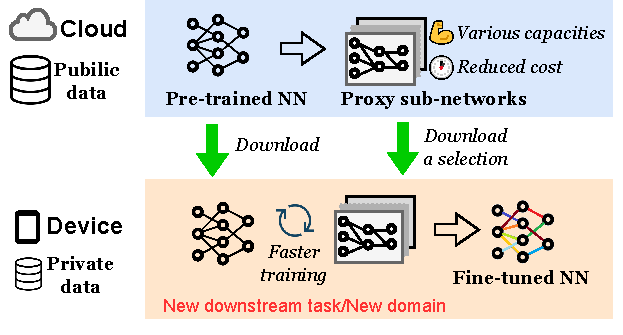
\includegraphics[width=0.98\linewidth]{figs/intro.drawio.pdf}
    
    \caption{How \sys works.}
    \label{fig:sketch map of PEFT}
    
\end{figure}


% Neural Networks (NNs) are a key enabler for mobile intelligence.
% Although NNs pre-trained on public large-scale cloud datasets have shown impressive foundational representational ability and generalization prowess, they still need on-device training to adapt to versatile and dynamic environmental domains or downstream tasks. 
% Many mobile/edge applications perform on-device fine-tuning, such as input personalization service ~\cite{xu2018deeptype}, sequential recommendation system ~\cite{han2021deeprec}, video analytics ~\cite{bhardwaj2022ekya}, voice assistant wake-up service ~\cite{siri}, etc.
% As such, on-device adaptation/personalization has recently become an eyeball-grabbing research domain ~\cite{}.

% On-device training is known to be much more resource-intensive than inference and often unaffordable on mobile devices. 
% \mwx{People might think fine-tuning is lightweight (as compared to pre-training). Show some numbers to back up?}
% For instance, using Raspberry Pi 4 to train Vision Transformer (ViT\_base) on Caltech-256 dataset can take over a month.
% Even on stronger devices with GPUs such as Nvidia Jetson TX2, the training on each image could still take over 30 seconds.
% Training ResNet-50 with one batch (batch size 32) takes 4.6 GB memory and 36.4 seconds on the smartphone MI 10. 
% The consumed energy equals to watching a 1080P-definition video for 111.2 seconds ~\cite{}.
% Fine-tuning tasks typically need thousands of iterations to converge, so the end-to-end training could take hours or days with unbearable energy consumption.
% Fortunately, recent advances in ML algorithms show that, with a large pre-trained NN, we can only update very few parameters (e.g., < 1\%) while achieve the similar accuracy, namely parameter-efficient training (PET).
% Popular PET algorithms include Linear probing ~\cite{}, Last $K$ layers ~\cite{}, Adapters ~\cite{}, LoRA ~\cite{}, and P-tuning ~\cite{}, etc. 
% PET methods are also scalable: the larger pre-trained model, the fewer parameters needing to be updated.

% According to our measurement in $\S$\ref{subsec:pre-measure}, PET indeed can effectively save storage and the need for data labels that are difficult to obtain on devices. 
% For instance, PET methods can achieve up to 17.32\% accuracy improvement with scarce data labels, and significantly reduce storage overhead by 5.6$\times$ when adapting to 6 different downstream tasks.
% Those factors take a giant step to make on-device fine-tuning practical. 

% \mwx{Highlight the issue in a separated paragraph}
However, such parameter efficiency does not translate coequal to time efficiency.
For instance, when fine-tuning ResNet50~\cite{he2015deep} on a MI 10 smartphone,
%using the Caltech-256~\cite{c256} dataset,
PET methods with less than 1\% trainable parameters still consume up to 96\% and on average 65\% of the training time compared to traditional full-model fine-tuning ($\S$\ref{subsec:pre-measure}, Figure~\ref{fig:time_measure}).
Such long training time results in more energy consumption, compromised user experience and delayed personalization service.
% \mwx{Talk about the consequences of long training time: more energy consumption, compromising user experience, delayed personalization service..}
Diving into the reason, we find out that the frozen layers dominate the training time (both forward pass and backward pass).
% \mwx{The frozen layers computing includes forward pass, but backward? Make it clear.}
For instance, when training Vision Transformer (ViT\_base)~\cite{dosovitskiy2021an} on NVIDIA Jetson TX2 with PET methods, the frozen layers account for 96.34\%–-99.59\% of the computation time (Table~\ref{table-frozenvstrainable}).
This observation provides a key opportunity that, as the compute-intensive layers are frozen during training, we can approximate them with cheaper ones (dubbed as \textit{Proxy sub-networks}, or \textit{subnets} in short).
% \mwx{Does't flow here. How about position it as one major challenge after introducing our key idea of subnet?}
% Yet, a simple, static replacement strategy could result in nontrivial degradation of convergence accuracy.
% For instance, replacing a ViT\_base with a structurally identical network that has significantly fewer FLOPs (e.g., < 50\%) for fine-tuning on the DTD dataset would result in a 29.11\% decrease in accuracy ($\S$\ref{subsec:ablation}, Figure ~\ref{fig:static}), and this number would further increase on more complex datasets.
% \mwx{say something like: while such approximation has been exploited for inference speedup, we are the first to apply it to on-device training.}
% While such approximation has been exploited for inference speedup~\cite{torchpruninggithub, krishnan2019structural}, we are the first to apply it to on-device training.

% To fully leverage this opportunity and further tap into the potential of parameter efficiency, we propose \sys, the first framework that effectively speeds up on-device PET through frozen-layer approximation.
% % \mwx{briefly describing the system model of \sys? goal is time-to-accuracy; cloud-device collboration; etc.}
% Its design goal is to achieve a better time-to-accuracy for on-device PET.
% To realize this goal, it works through cloud-device collaboration, leveraging the rich pre-training data to achieve NN approximation on cloud.

%\textbf{Challenge: static approximation significantly compromises accuracy.}
The main challenge in accelerating PET through NN approximation is that a \textit{simple, static replacement strategy} could result in nontrivial degradation of convergence accuracy.
For instance, approximating the frozen layers of a ViT\_base with a structurally identical network that has significantly fewer FLOPs (e.g., < 50\%) for fine-tuning on the DTD~\cite{dtd} dataset would result in a 29.11\% decrease in accuracy ($\S$\ref{subsec: sensitivity}, Figure ~\ref{fig:static}), and this number would further increase on more complex datasets~\cite{c256, ImageNet2012, ImageNet-21K}.
% \mwx{Provide intuitive reasons that echo to our design.}
This arises from two aspects: one is the error between the approximated network and the original network; the other is the compromised generalization ability due to the decreased model capacity.
% \mwx{last sentence needs to be polished}

In response, this work presents \sys, the first fast PET framework for mobile devices.
Instead of statically approximating the frozen layers during PET, the key idea of \sys is \textbf{data-aware dynamic approximation and routing.}
It's based on a key insight that the approximation of frozen layers must be more fine-grained, i.e., \textit{be dynamic for different training samples} during on-device training due to the high diversity of real-world data~\cite{ijcai2017p0735, he2019data, 10.1145/3495243.3517016, mercury2021sensys, canel2019scaling, 10.1145/2972413.2972423, 10.1145/3241539.3241557, pmlr-v162-mindermann22a, huang2018multiscale}.
More specifically, the training data exhibits opportunistic diversity in two unique aspects: \textit{difficulty} and \textit{importance}.
Difficulty is that some training samples are intrinsically easier to extract accurate and informative features from.
Importance is that some non-trivial training samples can facilitate faster convergence and better generalization.
We define them in our system model and show their ubiquitous presence in $\S$\ref{subsec:Opportunity: Training Data diversity}.

Realizing the above design needs to tackle two crucial challenges.
First, training-oriented subnets are hard to acquire: they must be with low approximation-induced accuracy loss, fast on-device execution speed, and a vast latency-accuracy trade-off space.
Second, as will be shown in $\S$\ref{subsec:Opportunity: Training Data diversity}, perceiving data diversity is non-trivial: data importance is stateful, and data difficulty is stateless but posterior. 
Online perceiving data diversity brute-force and forming routing strategy introduce undesirable extra time overhead.

\sys incorporates a two-stage design akin to prior literature~\cite{wen2023adaptivenet, Fang_2018, wang2022melon}:
on cloud (offline), it pre-generates the approximated subnets through public data;
on devices (online), it finetunes the models by judiciously routing the data to proper subnets.
%on cloud once and deploying these subnets along with the original NN to devices to assist on-device training. 
Specifically, the aforementioned challenges are tackled in the following two stages: the on-cloud pre-approximation and the on-device data-aware routing.

In the first stage, \sys employs a pruning-based fine-grained approximation method.
By gradually and structurally removing various components from the original NN, this method generates subnets with faster on-device execution speed.
The design differs significantly from prior inference-oriented pruning-based NN approximation~\cite{torchpruninggithub, krishnan2019structural}, since:
(1) It redesigns the pruning specification for PET, ensuring that the pruned NN structure is compatible with the parameter efficiency of the original NN.
(2) It recognizes that the requirements of NN approximation for training are more stringent (i.e., latent space alignment instead of trivial label alignment), thereby proposes a lightweight on-cloud retraining mechanism for more effective NN approximation.

In the second stage, \sys proposes an online-offline fused data perceiving and subnets routing method.
For data difficulty, it offline trains a transferable tiny policy model with public data as a substitute for online traversing all the subnets on devices;
For data importance, it builds an online monitor to employ observed training loss for zero-overhead estimation.
Specifically, the key insight of the policy model is that system-level compute-expensive estimation can be simplified using a data-driven black-box model.
It perceives data difficulty through a novel joint training mechanism with subnets.
Our method orchestrates the above perception (difficulty and importance) into subnets routing strategy during on-device training. 
Through these algorithm-system co-design, our method is accurate, end-to-end and cost-effective on devices.


\begingroup
\color{blue}
A further practical challenge is that on-device training may need to share resources with foreground inference.
For example, Ekya jointly supports live video inference and model retraining on edge GPUs~\cite{bhardwaj2022ekya}, while DaCapo targets concurrent inference and learning in autonomous systems such as drones and security robots~\cite{kim2024dacapo}.
For mobile applications, the TensorFlow Lite team also recommends running training that is not user-facing as a background task~\cite{tflite2021ondevicetraining}.
These examples motivate treating inference as a foreground service that should remain responsive while training proceeds.
When both share an accelerator, a training operation already in progress may delay a new inference request.
Waiting too conservatively, however, can leave gaps between requests unused and prolong training.
To use these gaps, \sys combines feature caching ($\S$\ref{subsec:feature-prefetch}) with foreground-aware scheduling ($\S$\ref{subsec:reorder}): it computes and stores features before the first trainable layer, and reorders feature computations according to the time available before the next inference request.
This complements proxy approximation by making better use of the compute time available to background training.
\par
\endgroup

We implemented \sys on multiple mobile/embedded devices including Nvidia Jetson TX2~\cite{tx2}, Raspberry Pi 4B~\cite{rpi}, MI 10 smartphone~\cite{mi10} and an NPU-empowered Commercial Off-The-Shelf (COTS) device Huawei Mate 30~\cite{HuaWei}.
We then evaluate its performance on four popular datasets~\cite{c101, c256, Dvg, dtd} and three representative NN architectures~\cite{he2015deep, howard2019searching, dosovitskiy2021an}.
% Neural Processing Units (NPUs) are designed for NN inference, and there is a significant gap compared to NN training. 
% But \sys can offload its computation of frozen layers to NPUs.
% From our experiment results, we have the following conclusions:
The results show that \sys consistently outperforms baselines in terms of time-to-accuracy, achieving up to 6.6$\times$ on-device speedup compared to traditional full model training and other competitive on-device training frameworks ~\cite{huang2023elastictrainer, 10.1145/3295500.3356156}, and 1.5$\times$--2.5$\times$ speedup compared to state-of-the-art PET methods.
Meanwhile, \sys does not compromise convergence accuracy and parameter efficiency.
Moreover, with the assistance of NPUs~\cite{Hiai}, \sys makes on-device training more practical on COTS devices: a medium-sized workload (ResNet50, Caltech-101) requires only 0.21 hours and 0.91 kJ of energy on Huawei Mate 30.

\begingroup
\color{blue}
We also evaluate ResNet50 training on Caltech-101 on a Jetson AGX Orin while foreground inference runs periodically.
At inference request periods of 105, 135, and 180\,ms, combining feature caching and reordering reduces the time for 12 training epochs, excluding evaluation, by 23.97--29.85\% compared with FIFO without caching ($\S$\ref{subsec:orin-periodic}).
\par
\endgroup

The major contributions are summarized below.

% \begin{itemize}
%     \item A key opportunity: frozen-layer approximation..
%     \item \sys: data-aware approximation and routing for efficient on-device PET.. key designs..
%     \item Experiments...
% \end{itemize}

\begin{itemize}[leftmargin=10pt,topsep=0pt]
\item We thoroughly explore a key opportunity for tapping into the potential of parameter efficiency: dynamic frozen-layer approximation, and propose the first on-device training framework with both time and parameter efficiency.
\item We introduce a pre-training-assisted on-cloud approximation method with high-quality speed-accuracy trade-offs, as well as an edge-tailored data perceiving and routing method that effectively and fully exploits the benefits brought by frozen-layer approximation.
\item We implement \sys on diverse mobile/edge devices and demonstrate its effectiveness through extensive experiments. \sys makes on-device NN adaptation and deployment much more practical for COTS devices in the era of deep learning.
\end{itemize}

% To sum up, the contributions of the paper include:
% We carry out the first parameter-efficient training measurement on actual mobile/embedded hardware.
% We demonstrate that it is a good fit to on-device fine-tuning for its effective memory/storage cost reduction and few-shot ability, but it is still time-consuming.
% \mwx{merged to above}
% We design a framework for time-efficient on-device PET named \sys by innovatively leveraging data diversity and neural network approximations.
% We demonstrate \sys's effectiveness through extensive experiments. 
% \sys makes on-device fine-tuning more practical for COTS devices.

% \mwx{
% The logic flow here:
% }

% Para-1: NN is a key enabler for mobile intelligence. To adapt the NNs to versatile and dynamic environmental domains, on-device training is important. Show some applications/scenarios.

% Para-2: On-device training is much more resource-intensive than inference (memory, time, energy, etc) and often unaffordable on mobile devices. Fortunately, recent advances in ML algorithms show that, with a large pre-trained model, we can only update very few parameters while achieve the similar accuracy. This method is also scalable: the larger pre-trained model, the fewer parameters needing to be updated.
% This is called parameter-efficient training (PET).

% Para-3: According to our measurement in Sec XX, PET indeed can effectively save memory footprint, storage, and data labels.
% Those factors take a giant step to make on-device training practical.
% However, a crucial obstacle remained is that the parameter efficiency does not bring as good time efficiency. For instance, XXX.
% We dive into the reason and find out that the frozen layers dominate the training time...

% Para-4: The above observation provides a key opportunity that, as the compute-intensive subnets are freezed during training, we can perhaps replace them with cheaper ones, e.g., through pruning techniques.
% Yet, a simple, static replacement strategy could result in nontrivial degradation of convergence accuracy.
% For instance...

% Para-5: In this work, we propose \sys, the first framework that effectively speeds up on-device PET.
% As shown in Figure 1, the key idea of \sys is to approximate the freezed sub-networks (the bottleneck) with more lightweight sub-networks.
% During training, the forward and backward propagation go through those proxy sub-networks, so the convergence is accelerated...
% There two underlying rationales:
% one is that modern NNs are often over-parameterized, especially for certain data points...
% the second is that training data is highly heterogeneous and they contribute differently to the model convergence.
% Specifically, we identify two primary factors of training data: importance and difficulty. <Explain the two factors.>
% Our experiments in Sec 2 show that XXX.

% Para-6: To speed up the training without compromising the accuracy, \sys needs to answer two key questions:
% (1) how to generate proxy subnets that can well approximate the original and exhibit rich accuracy-speed tradeoff;
% (2) how to dynamically route heterogeneous training data samples to the optimal proxy subnet.
% <Describe why they are difficult and prior work does not apply.>

% To address the first challenge, we propose to XXX.

% To address the second challenge, we propose to XXX.

% Implementation and evaluation.

% --------------------------------------------------------


% Neural Networks (NNs) have been widely applied to mobile and embedded devices for various tasks such as image and speech recognition.
% Typically, these neural networks are pre-trained on cloud datasets (e.g.  ImageNet, CCNet), and then deployed on edge devices.
% However, pre-trained NNs still require fine-tuning based on edge-side data for scenarios such as continuous learning or personalization. With increasing concerns about user data privacy protection, training NNs locally (i.e. on-device training) have attracted more attention.

% A common and efficient practice for on-device training is parameter-efficient fine-tuning (PEFT).
% It consistently freezes most of pre-trained parameters (usually more than 90\%) during on-device training, and only trains several selected layers (e.g. Batch Normalization, Bias, Convolution layers..) or newly added layers (e.g. Adapters, LoRA, Prefixes...).

% PEFT offers many advantages in on-device training. By freezing most parameters, it consumes less memory, requires fewer training samples, and is less prone to overfitting. 
% Moreover, PEFT allows the sharing of frozen pretrained parameters across different downstream tasks. 
% Only a small number of task-specific trainable parameters needs to be maintained for each task. This enables efficient adaptation to various downstream tasks on the edge.

% However, parameter efficiency does not translate to time efficiency. Despite PEFT’s ability to freeze over 90\% of the parameters, the actual wall-clock training time remains considerably long.
% %这两句话原封不动改的elastictrainer的写法
%     According to our preliminary measurements, using Raspberry Pi 4 to train vision transformer with 6 adapters (which means 1.77\% trainable parameters) on Caltech-256 dataset (15k training images) can take over 2 weeks.
% Even on stronger devices with GPUs such as Nvidia Jetson TX2, the training on each image could still take 30 seconds.

% % To speed up on-device training, existing works have proposed several methods. 
% % A possible solution is to offload training to low-precision hardware accelerators (e.g. Snapdragon Hexagon DSP), but their availability is limited on specific devices, and obtaining the low-precision format pre-trained parameters is challenging.

% xxx

% technique, contribution, challenge...

\section{background and motivation}

\subsection{Parameter-Efficient Training}
\label{subsec:PET}
\begin{table}[!t]
\caption{Comparisons of practical on-device PET methods. Model: ViT\_base.}
\label{table-PET Methods}
\centering
\footnotesize
\setlength{\tabcolsep}{2pt}
\begin{tabular}{@{}L{0.18\linewidth}L{0.24\linewidth}L{0.29\linewidth}L{0.23\linewidth}@{}}
\toprule
\textbf{PET Method} & \textbf{Trainable layers} & \textbf{Formula} & \textbf{Trainable Parameters} \\
\midrule
Linear Probing & The last linear layer & $y=x\cdot W+b$ & 0.69\% \\
\midrule
Last-K & The last $K$ layers & N/A & $\geq$8.3\% \\
\midrule
TS Layers & Task-specific layers (Norm. layers here) & N/A & 0.87\%--2.80\% \\
\midrule
Adapters & The inserted adapters & \mbox{$y=x+\sigma(x\cdot$}\newline\mbox{$W_{down})\cdot W_{up}$} & 0.71\% \\
\bottomrule
\end{tabular}
\end{table}

\begin{figure}[!t]
    \centering
    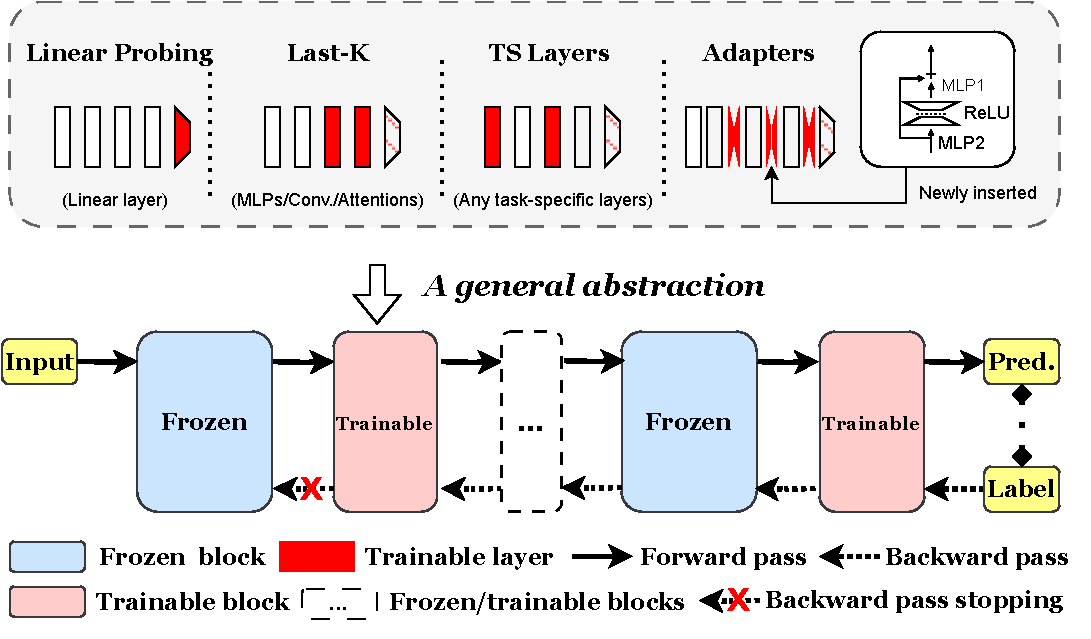
\includegraphics[width=0.98\linewidth]{figs/PET_abstraction.pdf}
    \caption{A layer-level general abstraction of PET. 
            }
    \label{fig:PET abs}
\end{figure}


Parameter-Efficient Training (PET) is a class of training techniques that aims to achieve performance comparable to full model training while freezing most pre-trained parameters.
Its parameter efficiency exhibits the following two pivotal characteristics:
(1) \textit{\textbf{Few adjustable parameters.}} Table ~\ref{table-PET Methods} provides a detailed presentation. 
(2) \textbf{\textit{Statically predefined trainable components.}} Trainable layers remain fixed during PET.

The rationale behind PET is that, through pre-training on large-scale datasets, the NN has learned a general inductive bias that is close to the downstream task (e.g., object contours in CV tasks).
Therefore, the expression ability brought by only adjusting a small number of parameters can adapt this bias to the downstream task.
PET is generally orthogonal to the deep model design and the training optimizers, and has gained lots of attentions in both academia and industry with the rise of large pre-trained models.

% \yws{Why there are different PET methods?}
%There is no silver bullet strategy for PET.
% On-device training tasks vary in their training time/energy constraint, acceptable test accuracy, and the amount of labeled training data, etc, thus could employ different PET methods.
We summarize widely used on-device PET methods in Table ~\ref{table-PET Methods}.
(1) ``Linear Probing'' means only fine-tuning the output layer and maximize the retention of pre-trained knowledge.%, which is the most resource-efficient method because it skips most backward pass. 
It can achieve accuracy close to or even better than fine-tuning all parameters according to recent studies, especially when data domains are close ~\cite{lin2022could, kornblith2019better, salman2020adversarially, kumar2022finetuning}.
(2) ``Last-K'' method tunes the last $K$ layers based on the rationale that layers close to the NN input learn generic transferable features ~\cite{MLSYS2019_e09d45e1, guo2019spottune, chatfield2014return}.
% It provides a trade-off between resource overhead and accuracy when there is a discrepancy between the source domain and the target domain, and is easy to implement from an engineering perspective (no extra added layers, continuous trainable blocks).
(3) ``TS layers'' means fine-tuning task-specific layers for specific downstream tasks, e.g., normalization layers for domain adaptation, prefix layers for tuning language models ~\cite{li2021prefix}, or text-embedding layers for adding new concepts into text-to-image diffusion models ~\cite{gal2022image}.
(4) ``Adapters'' method proposes to inject trainable, task-specific ``adapter'' modules between layers of the pre-trained model ~\cite{rebuffi2017learning, houlsby2019parameter}.
%An adapter module is $y = x + \sigma(x\cdot W_{down})\cdot W_{up}$, where $\sigma$ is the activation function, $W_{down}\in \mathbb{R}^{d_{in}\times d}$, $W_{up}\in \mathbb{R}^{d\times d_{out}}$, and $d<<d_{out}$.
% \yws{Summarized methods are all (1) layer level; (2) fixed during training.}
% \mwx{Can be futher compressed. Say something like: there other advanced PET techniques such as p-tuning and LoRa, yet they are mainly designed for LLMs and are not readily deployed on devices.}
There are other advanced PET techniques such as LoRA ~\cite{hu2022lora} and p-tuning ~\cite{liu-etal-2022-p}, yet they are mainly designed for very large models (e.g., LLMs) and are not readily well deployed on devices.

\noindent \textbf{A unified abstraction of PET.}
We unify the above PET methods into a general abstraction for the design of \sys.
As shown in Figure ~\ref{fig:PET abs}, the ``frozen block'' remains unchanged after pre-training, while the ``trainable block'' is optimized during downstream fine-tuning.
Each ``block’' contains as many consecutive frozen or trainable layers as possible.
In a PET training iteration, both the frozen and trainable blocks need computing the forward pass.
During the backward pass phase, the frozen blocks only need to compute the error gradients, while the trainable blocks not only compute the error gradients but also perform weight updates.
Note that when all the components preceding a specific trainable block are frozen, there is no need to continue computing the backward pass further.

% A layer-level PET model can be abstracted and visualized by Figure ~\ref{fig:PET abs}.
% In this representation, the “frozen weights” correspond to the pre-trained portion that remains unchanged, while the “trainable weights” encompass either the pre-trained layers or the new layers added during downstream fine-tuning.
% Commonly used trainable layers include Adapters, LoRA, Batch Normalization, Convolutional Layers, Linear layers, etc.
%  and introduce them as follows: 

% \noindent \textbf{Head.}
% A widely used PEFT method is to only fine-tune the the classification head ~\ref{}.
% Formally, assuming $X$ is the input feature, $W$ and $b$ are the weight and bias respectively, and $Y$ is the output, then the forward pass formula for this trainable part is $y = x\cdot W + b$.
% Trainable parameters account for only 0.69\% of all the model parameters.

% \noindent \textbf{Last-K.}
% Since most layers close to the NN input have learned the generic capabilities of feature extraction, Last-K method tunes the last K layers.
% It requires >=8.3\% trainable parameters because of its coarse granularity.

% \noindent \textbf{Adapters.} 
% Adapters method proposes to inject trainable, task-specific "adapter" modules between some layers of the pre-trained model.
% An adapter module is $y = x + \sigma(x\cdot W_{down})\cdot W_{up}$, where $W_{down}\in \mathbb{R}^{d_{in}\times d}$, $W_{up}\in \mathbb{R}^{d\times d_{out}}$, and $\sigma$ is the activation function.
% There is no silver-bullet configuration for how to insert adapters, and a common practice is to insert an adapter between each convolution/transformer encoder layer.
% Since $d<<d_{out}$, the trainable parameters only accounts for 0.87\%--2.80\% depending on the number of adapters.

% \noindent \textbf{LoRA.}
% LoRA, namely Low Rank Adapter, is a variant of adapters method, and is mostly used for fine-tuning large language models or diffusion models.
% It applies two "delta matrices" $A\in \mathbb{R}^{d_{in}\times d}$ and $B\in \mathbb{R}^{d\times d_{out}}$ to the pre-trained matrix $W\in \mathbb{R}^{d_{in}\times d_{out}}$, and the forward pass is $y = Wx+BAx$.
% LoRA is commonly applied to $W_{q}$,$W_{k}$,$W_{v}$ and $W_{o}$ of the multi-head attention, and requires 1.40\%--9.26\% trainable parameters.

% \noindent \textbf{TS Layers.}
% Specific down-stream tasks require fine-tuning specific layers, e.g., normalization layers for domain adaptation, prefix layers for LLM tuning, or text-encoder layers for adding new concepts to stable diffusion.
% Taking only tuning the normalization layers as an example, the trainable parameters only account for 0.71\% of all parameters.

% Due to the majority of weights being frozen, PET exhibits superior performance compared to traditional fine-tuning methods on edge devices with limited memory and fewer training samples.
% We conduct measurement studies and find several observations.


\subsection{Preliminaries}
\label{subsec:pre-measure}
\begingroup
\color{blue}
\noindent \textbf{PET reduces storage and memory costs.}
A shared pre-trained model can support multiple tasks by storing and switching only a small set of task-specific parameters~\cite{yuan2023rethinking, yang2023edgefm}.
These parameters can also fit within a device's Trusted Execution Environment~\cite{zhang2023no}.
Freezing parameters removes their gradient storage and reduces the activations retained for backpropagation~\cite{NEURIPS2020_81f7acab}.
For the measured PET configurations of ViT\_base, ResNet50, and MobileNetV3 at batch size 4, estimated training memory is 21.19--38\% of full-model training.

\noindent \textbf{Frozen layers still dominate training time.}
These savings do not translate into a comparable reduction in computation.
On a MI10 smartphone, training ResNet50 for one epoch on Caltech-256 takes 14.8 hours with full-model fine-tuning and 4.7 hours with linear probing.
Even the latter exceeds the reported average daily time available for smartphone training, 2.7 hours~\cite{xu2018deeptype}.
Across the measured PET configurations of ViT\_base and ResNet50 on Jetson TX2 at batch size 4, frozen layers account for 96.34--99.59\% of an iteration's computation time.
They still perform forward computation and, where needed, propagate gradients to earlier trainable layers.
Reducing this cost is therefore the main opportunity for accelerating on-device PET.
\endgroup

\subsection{Training Data Diversity}
\label{subsec:Opportunity: Training Data diversity}
\begingroup
\color{blue}
Replacing frozen layers with smaller networks can reduce computation, but using the same approximation for every sample can hurt accuracy ($\S$\ref{subsec: sensitivity}, Figure~\ref{fig:static}).
\sys instead uses differences in \textit{data difficulty} and \textit{data importance} to choose how much computation each sample receives.
As illustrated in Figure~\ref{fig:data_hetero}, blurred or obstructed images can be harder to extract features from, while a less familiar example can contribute more to learning than one the model already recognizes well.
\begin{figure}[!t]
    \centering
    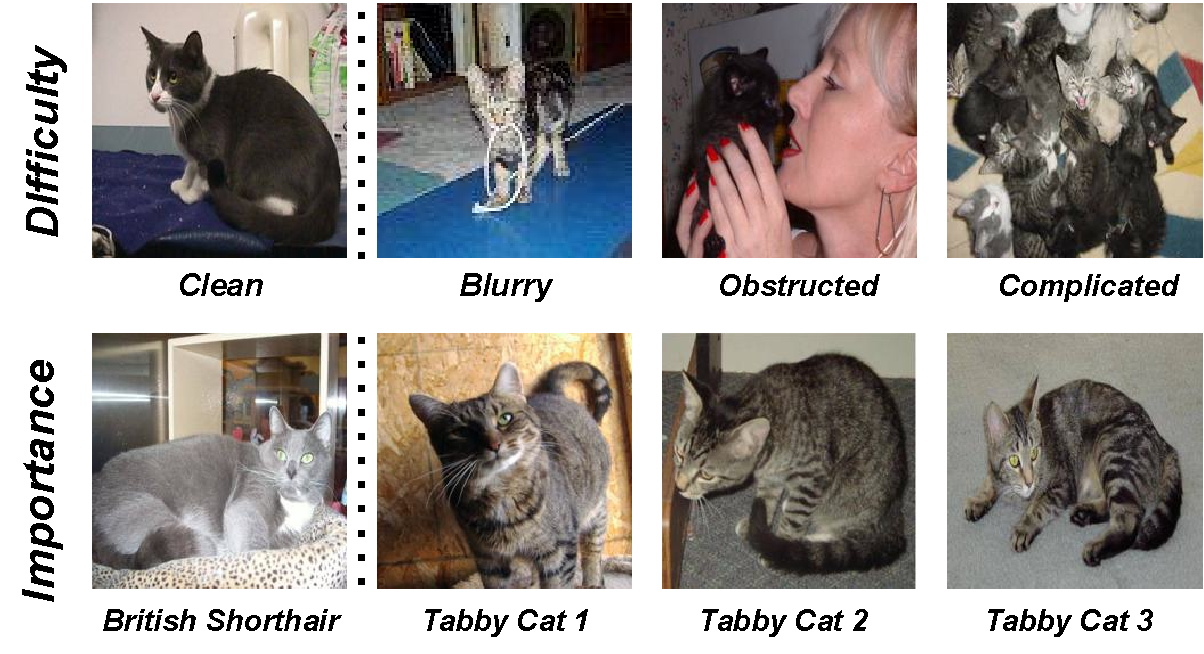
\includegraphics[width=0.92\linewidth]{figs/data_hetero.drawio.pdf}
    \caption{An intuitive example of data diversity. Dataset: Dogs vs. Cats; Class: cats.}
    \label{fig:data_hetero}
\end{figure}


\noindent \textbf{Data difficulty.}
Let $\mathcal{F}_0$ be the original network and $\{\mathcal{F}_n\}_{n=1}^{N}$ its progressively smaller proxies, constructed in $\S$\ref{subsec:proxy network generation}.
We measure difficulty by the smallest proxy that preserves the original network's features:
\begin{equation}
\begin{split}
\label{eq-difficulty_def}
\mathcal{\phi}(x) = \max\{n \in \{0,1,\ldots,N\}: \\
\mathcal{F}_n(x) \simeq \mathcal{F}_0(x)\}.
\end{split}
\end{equation}
Here, $\mathcal{F}_n(x)$ denotes the extracted features and $\simeq$ denotes sufficient feature similarity for PET.
A larger $\mathcal{\phi}(x)$ means that a smaller proxy can process $x$, so the sample is easier.

\noindent \textbf{Data importance.}
A sample's contribution to learning depends on the current model state.
We use its training loss as a practical indicator of this contribution, following prior work on loss-based importance estimation~\cite{mercury2021sensys, katharopoulos2017biased}:
\begin{equation}
\label{eq-importance_def}
\mathcal{\psi}(x,t) = l(x;w_t) = \mathcal{L}[\mathcal{F}(x;w_t),y],
\end{equation}
where $w_t$ is the model state at training iteration $t$, $y$ is the label, and $\mathcal{L}$ is the loss function.
Unlike difficulty, importance changes as the model learns.



\begin{figure}[!t]
	\centering
	\subfloat[Data difficulty\label{fig:difficulty}]{%
  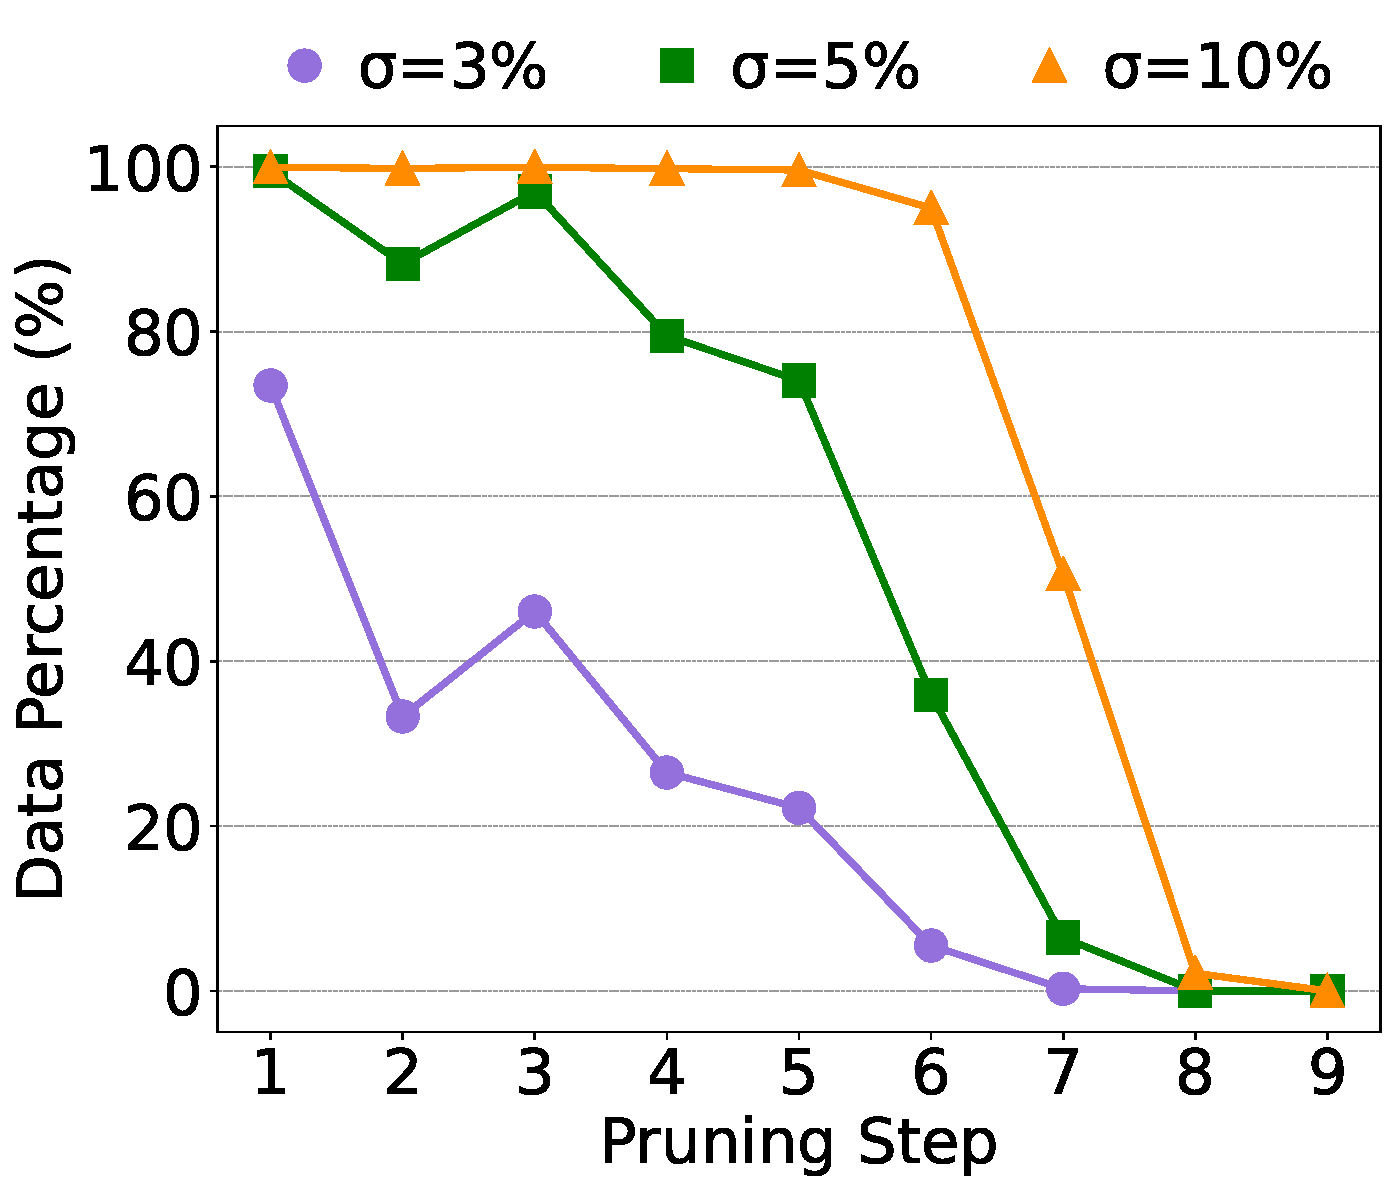
\includegraphics[width=0.47\linewidth]{figs/difficulty.pdf}}
	\subfloat[Data importance\label{fig:importance}]{%
  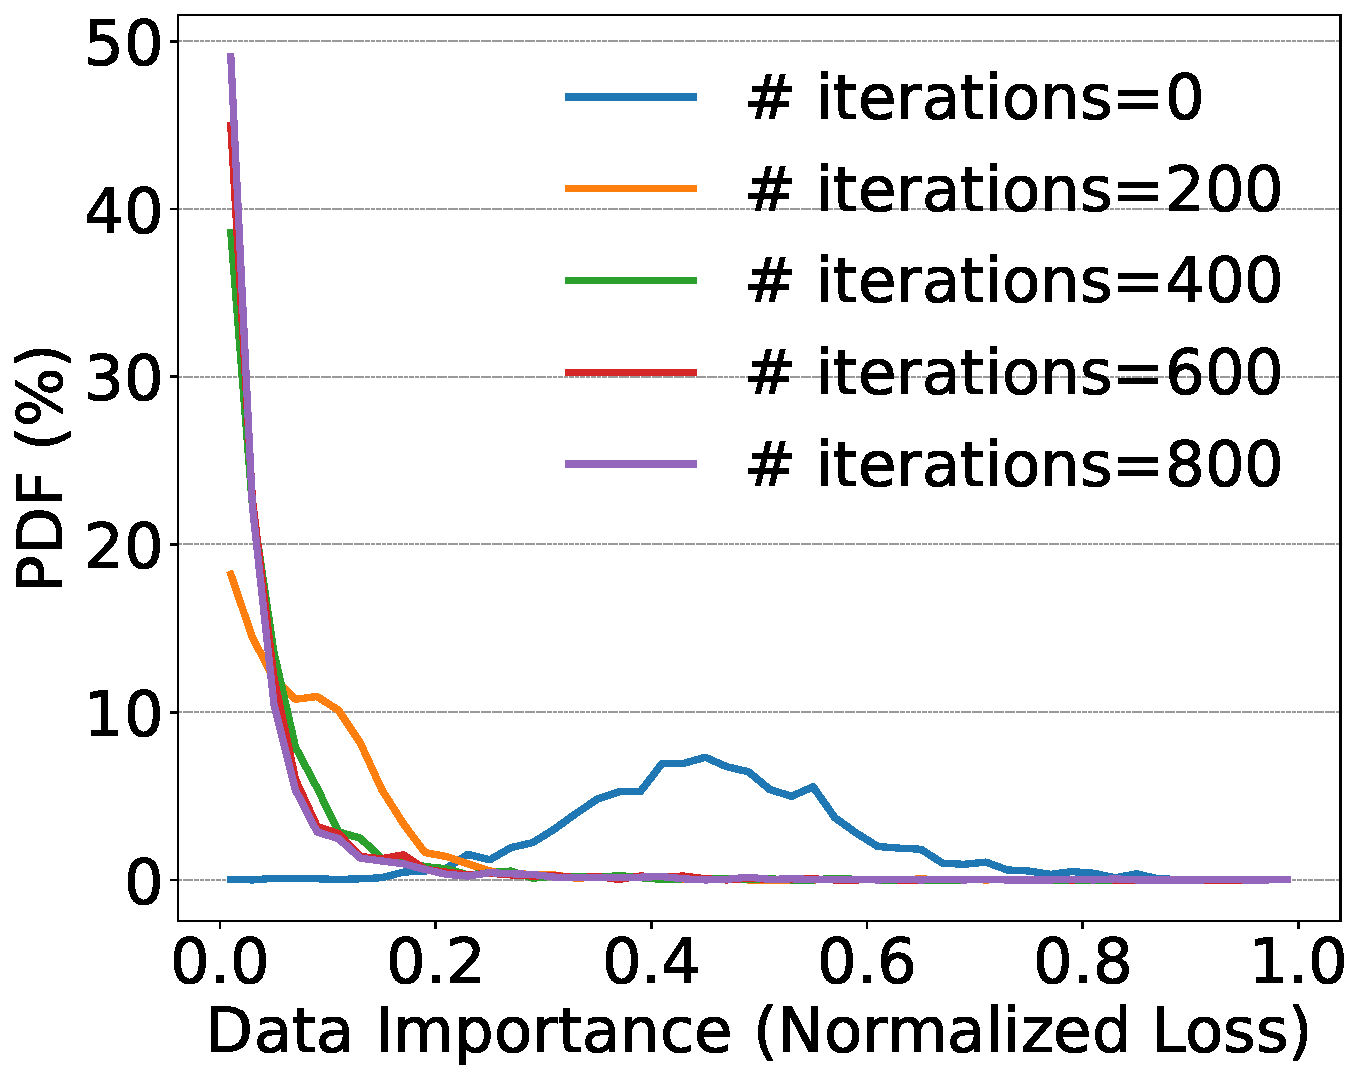
\includegraphics[width=0.47\linewidth]{figs/importance.pdf}}
        
	\caption{The diversity of training data from a statistical perspective. Model: ResNet50; Dataset: Caltech-101; Pruning step in (a): about 7\%--10\% FLOPs.
        }
        
\end{figure}

\noindent \textbf{Observed diversity.}
Figure~\ref{fig:difficulty} measures feature similarity using cosine similarity, with a threshold of $1-\sigma$.
At $\sigma=3\%$, more than 70\% of samples can use a smaller proxy, and more than 20\% can use one requiring only half the original network's computation.
The differences persist across the tested thresholds.
Figure~\ref{fig:importance} shows that importance also varies across samples and over time: after 200 iterations, high importance is concentrated in a small fraction of samples.
Together, these observations motivate using smaller proxies for easier or less important samples and retaining more computation for those that need it.
\endgroup

\section{\sys design}
\subsection{Overview}

\begin{figure*}[!t]
    \centering
    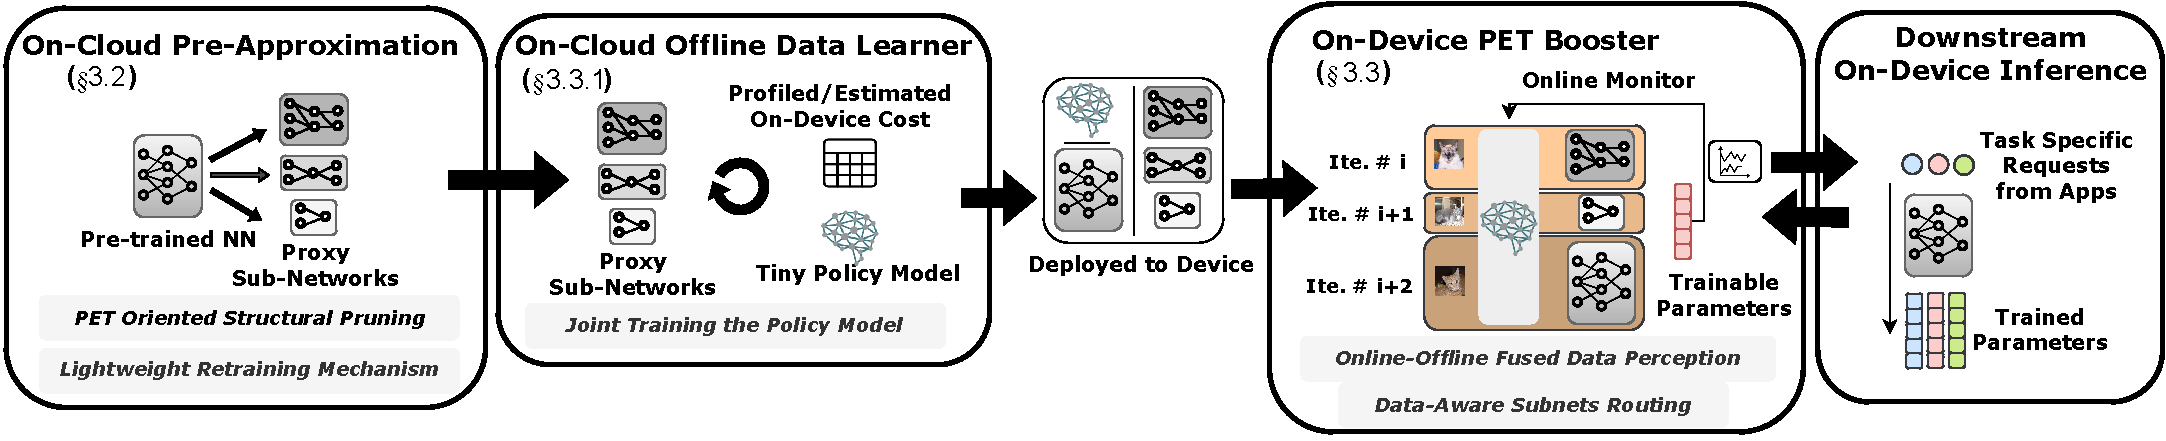
\includegraphics[width=0.995\textwidth]{figs/system_overview.pdf}
    \caption{An overview of \sys.}
    \label{fig:overview}
\end{figure*}


\noindent \textbf{System design goal.}
\sys is a cloud-device collaborated framework that aims to speed up the parameter-efficient on-device fine-tuning while not compromising the convergence accuracy (i.e., better time-to-accuracy) and the parameter efficiency.
% The key idea is to route ``easier'' and ``less-important'' data samples to more lightweight sub-networks that replace the ones in original NN that are frozen during fine-tuning.
% %through pre-generating lightweight proxy sub-networks on cloud and offloading heterogeneous training data to these proxies during on-device training.
% We refer to these lightweight sub-networks as ``proxy sub-networks'', or ``subnets'' in short, denoted by $\{F_{n}\}, n \in \{1, 2, \cdots, N\}$.
% To this end, \sys's design centers around two key questions:
% (1) At offline, how to generate lightweight and effective proxy sub-networks that well approximate the original ones?
% (2) During training, how to dynamically route heterogeneous training data to the proper proxy sub-networks?

% \mwx{define sub-network somewhere.}

\noindent \textbf{Workflow.}
Figure ~\ref{fig:overview} illustrates the two-stage simplified workflow of \sys.

At cloud offline stage, \sys generates proxy networks and prepares for the on-device training.
\ding{172} It first employs a PET oriented structured pruning to reduce the size of a given well-pre-trained original neural network. 
% It progressively removes neurons and layers, generating a series of smaller neural networks compared to the original model, i.e., \textit{proxy sub-networks}.
\ding{173} In order for the proxy sub-networks to participate in the training of the original network, a lightweight retraining mechanism is introduced to enable them to share the same latent space.
\ding{174} \sys profiles or estimates their actual on-device execution cost (including the original network) and records it in a latency score table.
% \mwx{only forward time is needed?}
% \yws{actually it's just a way to force the policy model to prefer lighter sub-networks. In my code I profiled the forward latency to realize it.}
\ding{175} Data difficulty is learned offline by an extremely lightweight end-to-end policy model.
\sys jointly trains it with the original network, proxy sub-networks, and on-device cost information using general public data on cloud.
% minimize the data selection overhead during on-device training, \sys also pre-trains a mini policy network on cloud.
% This policy network transfers the difficulty information learned from cloud data to device data basing on the assumption that the cloud pre-training data is sufficiently complex to reflect the general patterns of data distribution in the real world.
\ding{176} Finally, the original network, proxy sub-networks, and the policy model are all deployed together onto the device.

At device online stage, like other on-device continuous machine learning systems, \sys consists of two loosely-coupled runtimes, i.e., training runtime and inference runtime.
At training runtime, the plug-and-play trainable parameters are fine-tuned with device-collected data to adapt it to the drifted task or domain.
At inference runtime, the deployed NN serves as a one-size-fits-all foundation model shared by various applications.
\sys focuses on training runtime.
It dynamically routes training samples to different networks (the original network or the proxy sub-networks) according to an importance-and-difficulty-aware strategy.
This routing strategy for certain data sample $x$ is fused from two sources:
(1) The difficulty-based routing strategy from the policy model;
(2) The importance $\psi(x, t)$ monitored in near real-time.
% At this stage, we also perform opportunistic data skipping to avoid futile computation.
%takes into account the importance and difficulty of training data, dynamically routing different training data to the proper proxy networks. 
%It first inserts new trainable layers into the original NN before on-device training if necessary. 
% During the training process, it samples training data from the output of the policy network and selectively skips backpropagation based on the real-time importance of the training samples.
% Meanwhile, the importance of training samples will be fed back to the selection strategy of the proxy networks.


% \noindent \textbf{Key techniques.}
% While data diversity has been extensively studied for training optimizations ~~\cite{mercury2021sensys, guo2019spottune, 9888761, johnson2018training, katharopoulos2017biased}, we are the first to integrate it with neural sub-networks approximation to speed up on-device parameter-efficient training.
% \sys incorporates the following key techniques:
% (1) \textit{On-cloud pre-approximation}, which features a PET oriented pruning specification and a lightweight retraining mechanism ($\S$\ref{subsec:proxy network generation});
% (2) \textit{Data-aware proxy sub-networks routing}, which performs an edge-friendly online-offline fused data perception and dynamically routes data to appropriate sub-networks during on-device training ($\S$\ref{subsec:data-aware training});
% (3) \textit{Offline data difficulty learning}, which pre-learns data difficulty through a novel offline joint training method ($\S$\ref{subsubsec:policy model}).

\subsection{On-Cloud Pre-Approximation}
\label{subsec:proxy network generation}

% \begin{table}[!t]
\caption{Pruning space of different NN architectures.}
\label{table-pruning space}
\centering
    \smaller[2]
        \setlength{\tabcolsep}{1mm}{
        \begin{tabular}{c|c}
        \hline
            \textbf{Architecture} & \textbf{Pruning space} \\  
        \hline
             CNN & channels/layers \\
             Transformer & hidden sizes/attention heads/layers \\
        \hline
        \end{tabular}}
    
    
\end{table}


\textbf{Independent-Dimension Constrained (IDC) pruning.}
% the step size of pruning? the number of pruned networks?
There are many ways to obtain a lightweight approximation of the original network, such as pruning ~\cite{torchpruninggithub, huang2018multiscale}, quantization ~\cite{frantar2023gptq}, distillation ~\cite{aguilar2020knowledge}, and early exit ~\cite{xin-etal-2020-deebert}.
Intuitively, magnitude-based pruning provides the best trade-off between accuracy and computation among the above methods, since it is the most fine-grained.
Given a neural network with weights denoted as $W$, we can rank its element $w_{i}^{j}$ by the magnitude $\left\| \nabla l(x; w_{i}^{j})\cdot w_{i}^{j} \right\|$ on calibration samples $x$ and prune it.
Akin to prior arts~\cite{ma2023llmprunerstructuralpruninglarge, fang2023depgraphstructuralpruning}, \sys derives calibration samples from public general dataset (100 samples from ImageNet, by default).

To achieve actual speedup on device processors (e.g., ARM CPUs~\cite{HuaWei, mi10} or NVIDIA edge GPUs~\cite{tx2}) which typically do not support sparsity, the pruning must be structured.
However, traditional on-device acceleration oriented structured pruning~\cite{ofagithub, torchpruninggithub} lacks additional structural constraints, resulting in the approximated network being unable to participate in PET alongside the original network.
Figure~\ref{fig:pruning} shows an example of removing 20\% parameters from a PET structure in CNN.
A tuple (128, 128) represents the input/output dimensions of a layer.
If we arbitrarily prune any dimensions of a frozen layer (Figure~\ref{fig:pruning}(a)), the generated subnets cannot replace each other due to shape mismatch.

% \mwx{
% Clarify the novelty. Maybe re-organize this.
% }
To this end, \sys employs a dedicated pruning specification for PET, named Independent-Dimension Constrained (IDC) pruning (Figure~\ref{fig:pruning}(b)). 
Specifically, Given a PET network structure, IDC pruning identifies dimensions that are independent to its trainable blocks.
For a CNN block $y = \mathcal{C}_{r}(\cdots\mathcal{C}_{1}(x))$ where $\mathcal{C}_{r}(x)$ represents the $r_{th}$ convolutional layer, the independent dimensions are (1) $\mathcal{C}_{1}^{out}$, $\mathcal{C}_{2}^{in}$, $\cdots$, $\mathcal{C}_{r-1}^{in}$, if r is odd;
(2) $\mathcal{C}_{1}^{out}$, $\mathcal{C}_{2}^{in}$, $\cdots$, $\mathcal{C}_{r}^{in}$, if r is even.
For a Transformer block y = {\footnotesize $\mathcal{W}_{down}(\mathcal{W}_{up}(\mathcal{W}_{O}($$\mathcal{W}_{Q}(x)\mathcal{W}_{K}(x)\mathcal{W}_{V}(x))))$}, the independent dimensions are {\footnotesize $\mathcal{W}_{Q}^{out}$, $\mathcal{W}_{K}^{out}$, $\mathcal{W}_{V}^{out}$, $\mathcal{W}_{O}^{in}$, $\mathcal{W}_{up}^{out}$, $\mathcal{W}_{down}^{in}$}.
Following the above constraints, \sys performs magnitude-based pruning at a step size $d$ (by default 10\%, varied in $\S$\ref{subsec: sensitivity}).
For instance, proxy sub-network $\mathcal{F}_{1}$/$\mathcal{F}_{5}$ removes 10\%/50\% parameters compared to the original network $\mathcal{F}_{0}$ (and FLOPs are reduced in proportion).

% As shown in Figure ~\ref{fig:pruning}, given an original NN $\mathcal{F}_{0}$, \sys gradually performs structured pruning on its frozen parts with a step size of $d$.
\begin{figure}[!t]
    \centering
    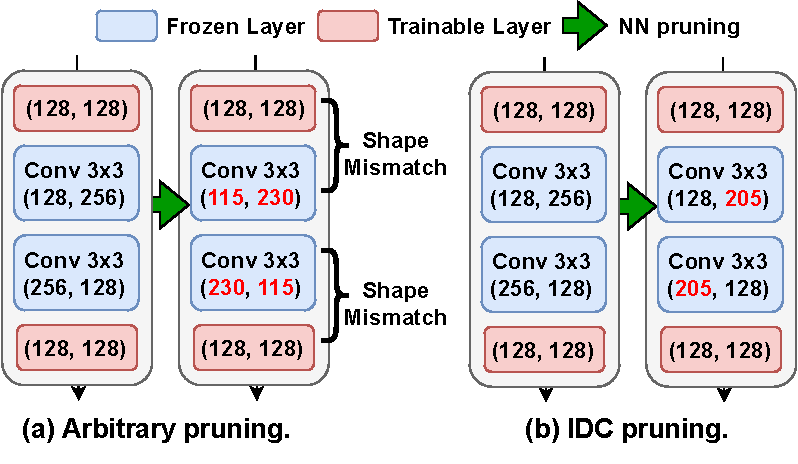
\includegraphics[width=0.88\linewidth]{figs/pruning.drawio.pdf}
    
    \caption{\sys only prunes independent dimensions of NNs. In doing so, proxy sub-networks are compatible with each other.}
    
    \label{fig:pruning}
\end{figure}

% \begin{table}[]
\footnotesize
\begin{tabular}{|l|l|}
\hline
Frozen Block &
  Independent Dimensions \\ \hline
y = $\mathcal{C}_{r}(\cdots\mathcal{C}_{1}(x))$ &
  \begin{tabular}[c]{@{}l@{}}$\mathcal{C}_{1}^{out}$, $\mathcal{C}_{2}^{in}$, $\cdots$, $\mathcal{C}_{r-1}^{in}$, if r is odd;\\ $\mathcal{C}_{1}^{out}$, $\mathcal{C}_{2}^{in}$, $\cdots$, $\mathcal{C}_{r}^{in}$, if r is even;\end{tabular} \\ \hline
\begin{tabular}[c]{@{}l@{}}y = $\mathcal{W}_{down}(\mathcal{W}_{up}(\mathcal{W}_{O}($\\ $\mathcal{W}_{Q}(x)\mathcal{W}_{K}(x)\mathcal{W}_{V}(x))))$\end{tabular} &
  \begin{tabular}[c]{@{}l@{}}$\mathcal{W}_{Q}^{out}$, $\mathcal{W}_{K}^{out}$, $\mathcal{W}_{V}^{out}$, \\ $\mathcal{W}_{O}^{in}$, $\mathcal{W}_{up}^{out}$, $\mathcal{W}_{down}^{in}$\end{tabular} \\ \hline
\end{tabular}
\end{table}

% \sys removes either some neurons of a layer (e.g., layers $b$ and $c$ in Figure ~\ref{fig:pruning}) or even the entire layer (e.g., layer $a$ in Figure ~\ref{fig:pruning}) based on the step size $d$.
% In detail, for convolution-based networks like ResNet and MobileNet, we remove channels; for Transformer-based networks like ViT, we reduce the hidden size of the MLP.
% We mainly verifies \sys on CNN and Transformer architectures, and their pruning space is as follows: 
% For CNNs (e.g., ResNet, MobileNet), we remove channels and even layers; For Transformers (e.g., ViT), we remove hidden sizes and also even layers.
% Structured removal of neurons leads to mismatched tensor shapes.
% In Figure ~\ref{fig:pruning}, ($b_{in}, b_{out}$) represent the input/output shape of a layer/block. 
% after pruning, two matrices $W_{in} \in \mathbb{R}^{n_{p}^{(l+1)} \times d_{in}^{(i)}}$ and $W_{out} \in \mathbb{R}^{d_{out}^{(i)} \times m_{p}^{(l+2)}}$ are added before/after each trainable layer separately to ensure the sharing of trainable layers across proxy networks with different shapes.
% After pruning, the output shape $b_{out}^{p}$ of layer $b$ does not match the input shape of the trainable block. 
% \sys introduces two matrices $W_{in} \in \mathbb{R}^{b_{out}^{p} \times b_{out}}$ and  $W_{out} \in \mathbb{R}^{c_{in} \times c_{in}^{p}}$ for each plugged PET block.
% $n^{(l)}$ and $m^{(l)}$ represent the output/input dimensions of the $l_{th}$ frozen layer, and $n_{p}^{(l)}$ and $m_{p}^{(l)}$ are the output/input dimensions after structural pruning. 
% $d_{in}^{(i)}$ and $d_{out}^{(i)}$ represent the input/output dimensions of the $i_{th}$ trainable layer.
% Note that the computational cost of $W_{in}$ and $W_{out}$ is also considered in the pruning step size $d$.
% In practice, we prefer to remove more parts from the layers closer to the network output.
In a nutshell, \sys's IDC pruning effectively provides approximations that achieve on-device speedup, and enables the generated proxy subnets to work seamlessly with each other.

% \noindent \textbf{Comparing IDC pruning with other approximations.}
% \mwx{
% (1) compared with pruning. (2) 
% }

\begin{figure}[!t]
	\centering
	\subfloat[Visualized feature\label{fig:shifting1}]{%
  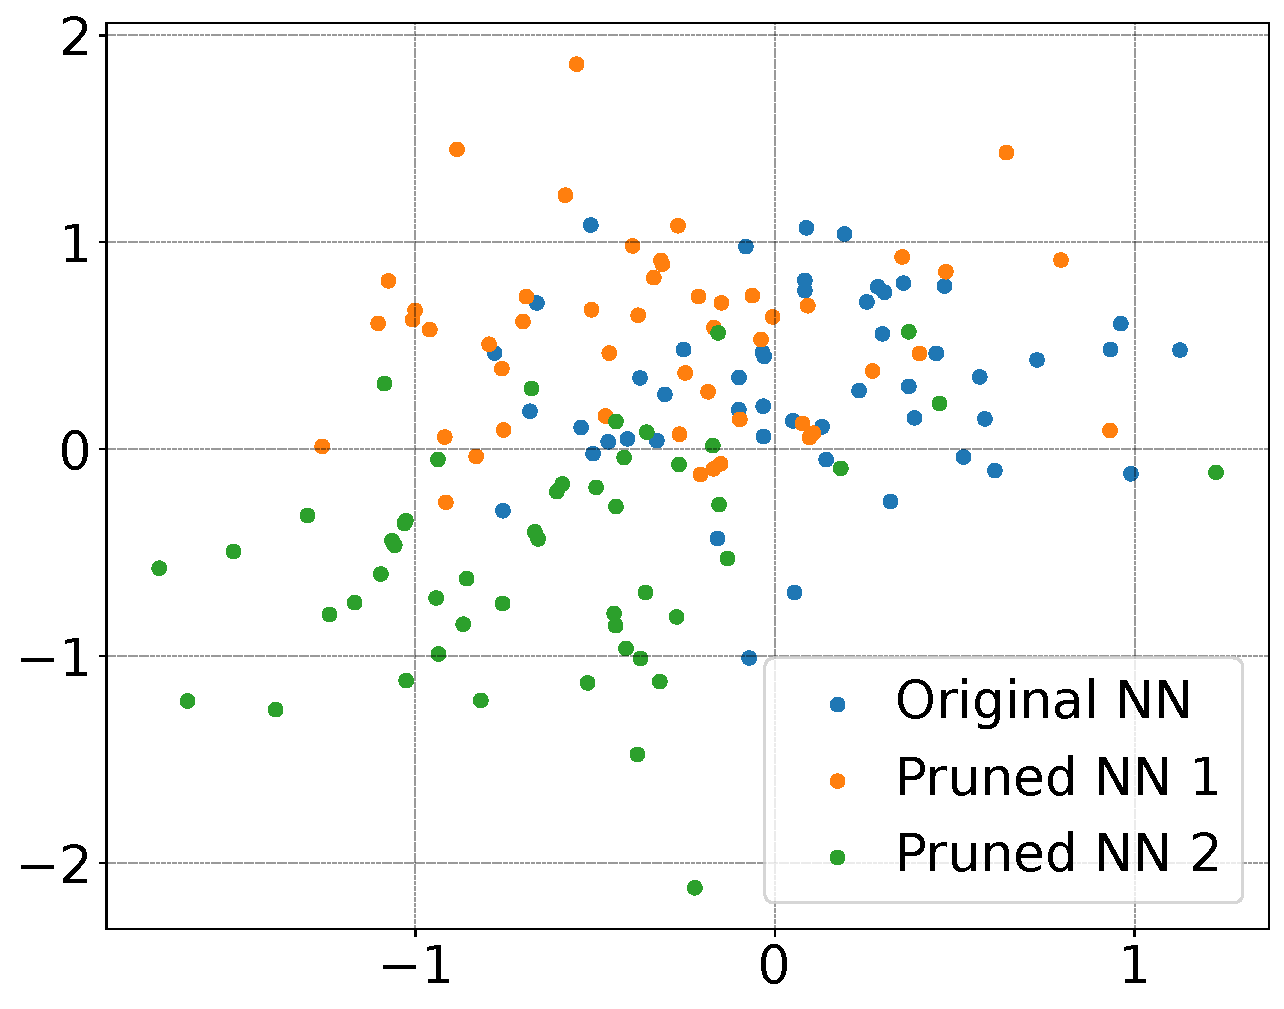
\includegraphics[width=0.45\linewidth]{figs/shifting1.pdf}}
	\subfloat[Vanilla FT vs. ours\label{fig:shifting2}]{%
  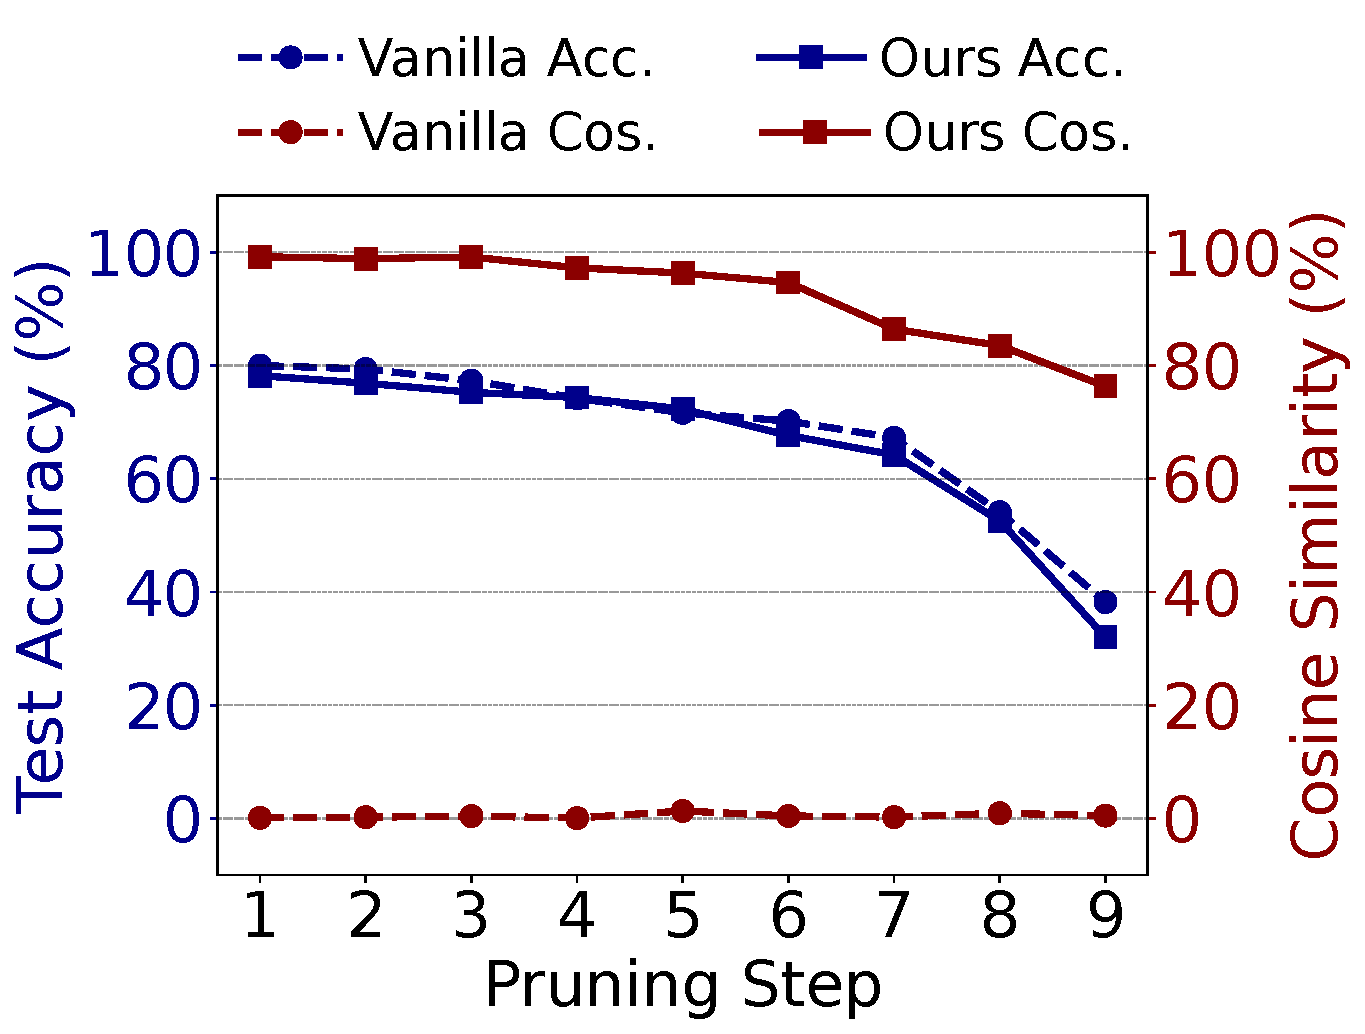
\includegraphics[width=0.51\linewidth]{figs/shifting2.pdf}}

	\caption{The latent space shift.
        (a) The visualized feature extracted by the original NN and 2 pruned subnets suffers a shift.
        (b) Test Accuracy and average cosine similarity between pruned and original NN.}
\end{figure}

\noindent \textbf{Latent space alignment through lightweight retraining.}
Unfortunately, the proxy sub-network pruned by IDC pruning is still not a good (accurate) approximation.
We dive into the reason and find out that the requirements of NN approximation for training are more stringent.
In Figure ~\ref{fig:shifting1}. we reduce the dimensionality of the latent space through PCA (Principal Component Analysis) and visualize it.
The latent spaces exhibit a gap.
It means that, though the pruned network may retain the ability to do inference (e.g., predict a dog as ``dog''), the feature feed to the shared trainable block may be tortured and thus noisy for PET.
To this end, we propose an enhanced alignment method with a dedicated regularization term. 
For each proxy sub-network $\mathcal{F}_{n}$, $n \in \{1, 2, \cdots, N\}$, we respectively minimize
% not a formula, too. formulize it latter.
% \begin{align}
% 	\mathcal{L} = -\sum_{i=1}^{k} y_i \log \left( \frac{e^{z_i}}{\sum_{j=1}^{k} e^{z_j}} \right) + \sum_{r=1}^{R}\lambda_{r} (h_{0}^{r} \otimes  h_{n}^{r}),
% 	\label{eq-loss_cosine_finetune}
% \end{align}
\begin{align}
%
	\mathcal{L} = \mathcal{L'} + \sum_{r=1}^{R}\lambda_{r} (h_{0}^{r} \otimes  h_{n}^{r}),
%
	\label{eq-loss_cosine_finetune}
\end{align}
where $\mathcal{L'}$ is vanilla fine-tuning loss (e.g. cross entropy loss), $h_{n}^{r}$ is the hidden state before the $r_{th}$ trainable block (i.e., the input), $R$ is the number of trainable blocks, $ \otimes $ is an operator to compute similarity, and $\lambda_{r}$ is the scale factor (1.0 by default).
% $L_{CoE}$ is the cosine-embedding loss function, and $h_{j}^{i}$ represents the activation of the $i_{th}$ trainable layer of the $j_{th}$ proxy network.
% $\lambda_{i}$ is the scale factor, and $I$ is the number of trainable layers.
% We use cosine similarity to measure the similarity between $h_{0}^{r}$ and $h_{n}^{r}$.
% , i.e.,
% \begin{align}
%         h_{0}^{r} \otimes h_{n}^{r} = \frac{h_{0}^{r} \cdot h_{n}^{r}}{ \left\| h_{0}^{r} \right\| \left\| h_{n}^{r} \right\|}.
% \end{align}
% It is easier to converge compared to  mean squared error (MSE) from our observation.
\textbf{\textit{Effectiveness}.}
\yws{
Figure ~\ref{fig:shifting2} reports the test accuracy and latent space alignment of vanilla fine-tuning and our method.
After vanilla fine-tuning, the features can only maintain a good test accuracy but compromise the alignment, while our method achieves both.
We integrate our alignment method into a lightweight retraining mechanism triggered after pruning.
We also conduct experiments on significance of key designs in $\S$\ref{subsec: sensitivity}. 
}
% \mwx{
% Clarify the novelty.
% }


% \mwx{Add the following parts: }

% \noindent \textbf{Necessity and novelty of the key designs.}
% \mwx{
% (1) Necessity of IDC pruning. Without 
% }

\noindent \textbf{Overhead analysis.}
Firstly, it is worth noting that the pre-approximation process takes place on cloud, which is relatively resource-abundant.
Secondly, compared to the resource-intensive pre-training process, the cost of our pruning and retraining is much lower.
We only perform 3 epoch of retraining for each sub-network.
% For instance, pruning and retraining 10 proxy sub-networks for a ResNet50 consumes just 1\%-10\% additional GPU hours. 
Furthermore, this process is executed one-shot: these approximated public proxy sub-networks can be shared by various devices.

\subsection{On-Device Data-Aware Routing}
\label{subsec:data-aware training}

\noindent \textbf{Profiling data diversity: undesirable system overhead.}
According to equation ~\ref{eq-difficulty_def}, acquiring the difficulty of a training sample is ``posterior'': it demands up to $N$ forward passes in the worst case (whereas the training itself involves just one forward/backward pass), which is unacceptable on devices.
According to equation ~\ref{eq-importance_def}, data importance is ``stateful'': it is influenced by the current training state $t$, which incurs additional forward computations~\cite{mercury2021sensys} for accurate perception because of the issue of ``staleness'' (Figure ~\ref{fig:stale}).

\noindent \textbf{Online-offline fused data perception.}
Inspired by ML-based system optimization efforts, such as database query optimization~\cite{marcus2021bao, negi2021steering} and matrix multiplication optimization~\cite{fawzi2022discovering}, we decouple the perception of data difficulty to the on-cloud offline phase.
Specifically, we design a data-driven black-box tiny model, referred as policy model $\Omega$.
The model is offline trained and performs online inference.
The design and training details are shown in $\S$\ref{subsubsec:policy model}.
As a stateful attribution, data importance is still perceived online.
We use the current forward pass to get real-time data importance.
\yws{
At a certain iteration, the importance comes from the current network state by reusing the training loss, and the details are presented in the following Algorithm~\ref{alg:on-device_training}.
}
% \mwx{Elaborate what the ``hitchihike'' means here.}

The above online-offline fused data perception incurs negligible online overhead.
Most of the additional overhead comes from the online inference of the tiny policy model.
For instance, on NVIDIA Jetson TX2, the per-sample perception time for ResNet50 is only 0.6 ms on average, which is less than 1\% of an entire training iteration.

\begin{figure}[!t]
    \centering
    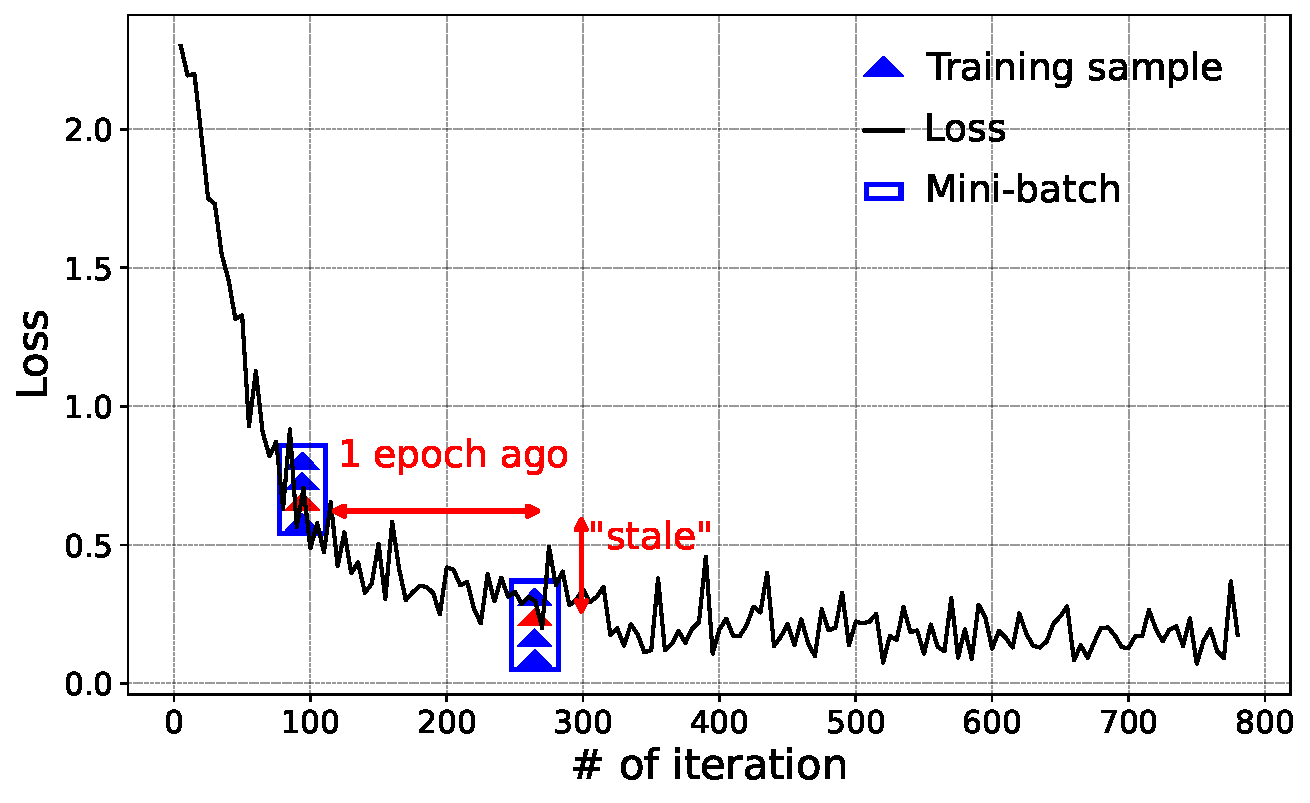
\includegraphics[width=0.82\linewidth]{figs/stale.pdf}
    \caption{The precision of data importance estimation. The estimate of specific training sample (red triangle) from the previous forward pass becomes ``stale'' as the training progresses.}
    \label{fig:stale}
\end{figure}

\begin{algorithm}[t]
\scriptsize
\SetAlgoNlRelativeSize{-1}
% \SetAlgoNlRelativeSize{-3}
\SetAlgoNoEnd
\SetKwProg{Fn}{Function}{~}{end}
\SetKwInOut{Input}{input}\SetKwInOut{Output}{output}\SetKwInOut{Variable}{Variable}
\Input{\footnotesize
    \textcolor{blue!85!black}{$\{\mathcal{F}_{n}\}$}, $n \in \{0, 1, 2, \cdots, N\}$; \textcolor{blue!85!black}{$\Omega$}; On-device dataset \textcolor{blue!85!black}{$D$};
}
\Output{\footnotesize
    Fine-tuned \textcolor{blue!85!black}{$\mathcal{F}_{0}$};
}
\BlankLine
\Fn{\footnotesize \textcolor[RGB]{170,144,6}{data\_aware\_training():}}{
    % $loss\_func$ \textcolor{red!85!black}{$\leftarrow$} $CrELoss()$; 
    % \tcc{Initialization}
    \textcolor{blue!85!black}{$train\_loader$} \textcolor{red!85!black}{$\leftarrow$} \textcolor{blue!85!black}{$D$}, \textcolor[RGB]{170,144,6}{$Policy\_sampler()$};
    \textcolor{blue!85!black}{$\theta$} \textcolor{red!85!black}{$\leftarrow$} \textcolor{green!50!black}{$-1$}; 
    \textcolor{blue!85!black}{$m$} \textcolor{red!85!black}{$\leftarrow$} \textcolor{green!50!black}{$0.8$}\;
    \For{\textcolor{blue!85!black}{$epoch$} \textbf{in} \textcolor{blue!85!black}{$epochs$}}{
        \For{ \textcolor{blue!85!black}{$data$} \textbf{in} \textcolor{blue!85!black}{$train\_loader$}}{
            \textcolor{blue!85!black}{$X$}, \textcolor{blue!85!black}{$n$} \textcolor{red!85!black}{$\leftarrow$} \textcolor{blue!85!black}{$data$}; \textcolor{green!60!black}{\tcp{mini-batch and routing strategy}}
            \textcolor{blue!85!black}{$l$} \textcolor{red!85!black}{$\leftarrow$} \textcolor{blue!85!black}{$X$}, \textcolor{blue!85!black}{$\mathcal{F}_{n}$}; \textcolor{green!60!black}{\tcp{get loss by \textbf{one} sub-network $\mathcal{F}_{n}$}}
            \textcolor{green!60!black}{\tcc{Opportunistic data skipping}}
            \For{\textcolor{blue!85!black}{$x$} \textbf{in} \textcolor{blue!85!black}{$X$}}{
                \lIf{ \textcolor{blue!85!black}{$l[x]$} \textcolor{red!85!black}{>} \textcolor{blue!85!black}{$\theta$}}{
                    \textcolor{blue!85!black}{$l[x]$}\textcolor[RGB]{170,144,6}{$.bp()$};
                    \textcolor{blue!85!black}{$sampler$}\textcolor[RGB]{170,144,6}{.\textit{adjust}(}\textcolor{blue!85!black}{$x$}, \textcolor{green!50!black}{$0$}\textcolor[RGB]{170,144,6}{)}
                }\lElse{
                    \textcolor{blue!85!black}{$sampler$}\textcolor[RGB]{170,144,6}{.\textit{adjust}(}\textcolor{blue!85!black}{$x$}, \textcolor{green!50!black}{$1$}\textcolor[RGB]{170,144,6}{)}
                }
            } 
            \textcolor{green!60!black}{\tcc{Momentum-based filtering threshold}}
            \textbf{if} \textcolor{blue!85!black}{$\theta$}==\textcolor{green!50!black}{$-1$} \textbf{then} \textcolor{blue!85!black}{$\theta$} \textcolor{red!85!black}{$\leftarrow$} \textcolor{blue!85!black}{$l$}; \textbf{else} \textcolor{blue!85!black}{$\theta$} \textcolor{red!85!black}{$\leftarrow$} \textcolor{blue!85!black}{$m\theta$} + \textcolor{blue!85!black}{$(1-m)l$}\;
            \textcolor{green!60!black}{\tcc{Synchronizing trainable blocks}}
            \textbf{for} \textcolor{blue!85!black}{$i$} \textbf{in} \textcolor{blue!85!black}{\{0, 1, $\cdots$, $N$\}} \textbf{ do } \textcolor{blue!85!black}{$\ensuremath{\mathcal{F}_{i}}$} \textcolor{blue!85!black}{$.trainable$} \textcolor{red!85!black}{$\leftarrow$} \textcolor{blue!85!black}{$\ensuremath{\mathcal{F}_{n}}$} \textcolor{blue!85!black}{$.trainable$};
        }
    }
    \textbf{return} \textcolor{blue!85!black}{$\ensuremath{\mathcal{F}_{0}}$};
}
% \Fn{\footnotesize{\textcolor[RGB]{170,144,6}{Policy\_sampler():}} \scriptsize{\textcolor{green!60!black}{\tcp{called once per epoch}}}}{
%     aaa
% }

\Fn{\footnotesize{\textcolor[RGB]{170,144,6}{Policy\_sampler():}} \scriptsize{\textcolor{green!60!black}{\tcp*[h]{called once per epoch}}}}{
    \textcolor{blue!85!black}{$P$} \textcolor{red!85!black}{$\leftarrow$} \textcolor{blue!85!black}{$\Omega$}, \textcolor{blue!85!black}{$D$}; \textcolor{green!60!black}{\tcp{a list, routing strategy $n$ = $P$[index of $x$]}}
    \Fn{\footnotesize{\textcolor[RGB]{170,144,6}{adjust(\textcolor{blue!85!black}{$x$}, \textcolor{blue!85!black}{$\epsilon$})};} \scriptsize{\textcolor{green!60!black}{\tcp*[h]{adjust $x$'s routing strategy by $\epsilon$}}}}{}
    % $policy\_list$ \textcolor{red!85!black}{$\leftarrow$} adjust the $policy\_list$ based on the filter \; 
    \textcolor{blue!85!black}{$Q$} \textcolor{red!85!black}{$\leftarrow$} \textcolor{blue!85!black}{$[0:\textcolor[RGB]{170,144,6}{len(}D\textcolor[RGB]{170,144,6}{)}]$}; \textcolor{green!60!black}{\tcp*[h]{a list storing sampling order of $D$}} \\
    \textcolor{blue!85!black}{$Q$}\footnotesize{\textcolor[RGB]{170,144,6}{.\textit{sort}()}\textcolor[RGB]{170,144,6}{.\textit{shuffle}()}}; \scriptsize{\textcolor{green!60!black}{\tcp*[h]{sort by policy, shuffle in same policy}}} \\
    \textbf{return} \textcolor{blue!85!black}{$sampler$}; \textcolor{green!60!black}{\tcp*[h]{for $train\_loader$ to sample mini-batch}}
}

\caption{Data-aware on-device training.}
\label{alg:on-device_training}
\end{algorithm}



\noindent \textbf{Data-aware subnet routing.}
Based on the perceived data diversity, \sys judiciously assigns training samples to proper subnets.
In general, we obtain a difficulty-based routing strategy from the policy model, and adjust this strategy with real-time data importance.
This strategy is dynamic: during training, each mini-batch selects the most suitable sub-network for itself.

In detail, we demonstrate our routing strategy by describing the on-device training procedure of \sys in algorithm ~\ref{alg:on-device_training}.
It receives \{$\mathcal{F}_{n}$\}, $\Omega$, and the on-device dataset $D$, and finally outputs the fine-tuned network $\mathcal{F}_{0}$.
The routing strategy is maintained by function $Policy\_sampler()$, which samples mini-batches and ensures that samples within the same mini-batch share the same level of difficulty.
After getting the output of $\Omega$ (line 17), we online adjust it by function $adjust()$ (line 18, line 8--10).
Both $\Omega$ and $adjust()$ adhere to the principle of minimizing computation for easier or less important data.
% \yws{An example? not clear here.}
The main body of on-device training is in function $data\_aware\_training()$.
During each iteration, we sample a mini-batch $X$, obtain its routing strategy $n$, and select a proxy sub-network $\mathcal{F}_{n}$ for training (line 5--6).

% \mwx{Give high-level description of our routing strategy, especially how data difficulty and importance affect the routing.}

% \mwx{Focus on following questions: at high level, why the data difficulty needs to be learned, while importance does not? How data importance is calculated (data difficulty details can go later)?}

% \noindent \textbf{Opportunistic Data Skipping.}
% \begin{figure}[!t]
    \centering
    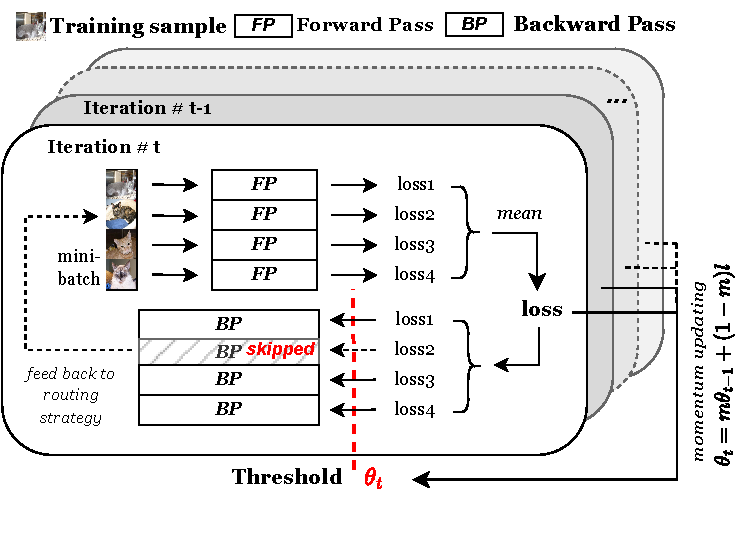
\includegraphics[width=0.82\linewidth]{figs/importance_filter.pdf}
    
    \caption{\sys opportunistic data skipping.}
    \label{fig:filter workflow}
    
\end{figure}

% \noindent \textbf{Skipping . }
In line 7--12, we further filter unimportant data from back-propagation.
Training data that has already well converged is all pain and no gain: it consumes computational resources while contributes little to convergence.
% Fortunately, our design of data-aware subnets routing has provided us with the opportunity to skip over these data points when profiling data importance.
%As shown in Figure ~\ref{fig:filter workflow}, 
We skip the backward pass stage of training sample $x$ by comparing its data importance to a threshold $\theta$.
To perform stable and solid filtering, $\theta$ is dynamically updated based on momentum.
Let $\theta_{t}$ be the threshold at iteration $t$, $m\in[0, 1)$ be the momentum coefficient, $l$ be the loss of current iteration, then we get
\begin{align}
	\theta_{t+1} = m\theta_{t} + (1-m)l.
	\label{eq-filter_thres}
\end{align}
Usually, $\theta$ is initialized as the loss from the first iteration, and $m$ is relatively large (e.g., 0.8, our default).
After filtering, we then feed the profiled importance back to routing strategy by function $adjust()$.

\noindent \textbf{Asynchronous subnets loading. }
Notably, only \textit{one} proxy sub-network is involved in a training iteration, so keeping all networks in device memory simultaneously is not necessary.
Thereby, \sys asynchronously loads the subnet of next iteration during the current iteration.
Such a loading is overhead-free in training time as computation time is much longer than loading.
% \mwx{About 0.8 page. Move Sec 3.5 \& 3.6 here.}
In doing so, the peak memory usage of our framework is nearly identical to PET, with only additional buffers for maintaining weights of a proxy sub-network of next iteration (detailed in $\S$\ref{subsec: energy}).

% \mwx{This paragraph is relatively independent.}

\subsubsection{\textbf{Learned Data Difficulty}}
\label{subsubsec:policy model}
Here we focus on the details of how data difficulty is obtained through offline-online collaboration.
% \mwx{Explain the following things in rationale: (1) why data difficulty can be learned (2) How does the learning work (3) Why it should be learned. Especially, the learning is also free of the need for defining the similarity constraint $\sigma$, since the feature similarity is end-to-end represented by the learning loss.}
\yws{
As discussed before, a straightforward way to perceive the data difficulty is to run all (pre-trained) proxy networks for a data sample to compare the features (recall Equation~\ref{eq-difficulty_def}).
On one hand, running all proxy networks is unacceptable on devices, and the constraint to determine whether $\mathcal{F}_{n} (x) \simeq \mathcal{F}_{0}(x)$ also involves ad-hoc designs (e.g., using cosine similarity; setting threshold $\sigma$, etc.).
On the other hand, as an intrinsic characteristic standalone to training state, intuitively the data difficulty does not have to be perceived online.
}
% \mwx{About 0.7 page. Move Sec 3.4 here. What's the cost of offline training?}

% \mwx{This section focuses on the details of how data difficulty is obtained through offline-online collaboration.}

%(为什么都有效，为什么我们同时考虑)
% \subsection{Difficulty-based Data-to-subnets Routing Policy Model}
% \label{subsec:the policy model}
% needs to be renamed, current name leads to misunderstanding.

%\textbf{The need for a lightweight routing strategy.}
% During on-device training, obtaining the difficulty $\phi(x)$ of each training sample $x$ and selecting an appropriate proxy sub-network $\mathcal{F}_{n}$ would introduce additional overhead.
% Equation ~\ref{eq-difficulty_def} already implies the inherent complexity of this issue.
% % By equation ~\ref{eq-difficulty_def}, naive approaches like directly comparing the features extracted from different proxy sub-networks result in significant computational overhead due to the need to perform forward pass for each sample on each proxy sub-network in every training iteration.
% A naive approach that directly compares the features extracted from different proxy sub-networks needs to perform a forward pass for each sample and proxy sub-network, thus incurring unacceptable overhead.
% %Taking the example of training a ResNet50 model with 1 adapter using 3 proxy sub-networks with a pruning step size of 20\%, obtaining the data difficulty for each iteration takes 168 ms, while the training process itself only takes 62 ms.

% \mwx{What's the rationale? Need more description of Fig 10 and make this technique clearer (it seems to be the most novel one).}
\noindent \textbf{``Learned data difficulty'' through a lightweight policy model.}
\yws{
\sys's response is an end-to-end learning for data difficulty with implicitly determining $\mathcal{F}_{n} (x) \simeq \mathcal{F}_{0}(x)$ by the learning loss.
}
We design a lightweight policy model $\Omega$ to end-to-end learn the data difficulty.
The input of the policy model is a training sample $x'$ downsampled from $x$ (\yws{i.e., resizing the input using interpolation}), and the output is a one-hot vector $\Omega(x') \in \mathbb{R}^{1 \times (N+1)}$. 
% \mwx{Details of downsample.}
$\Omega$ is tiny because we only use a small fraction of the original network $\mathcal{F}_{0}$. 
For instance, we use 2 residual blocks for ResNet50, 2 basic blocks with 2 depthwise separable convolutions each for MobileNetV3, or 1 encoder layer for ViT base, and each module has a smaller size compared to the original network. 
The total parameter count is less than 5\% of the original network.\footnote{
Although increasing the model size may lead to better routing performance, the benefits diminish marginally, while the online inference overhead shows no marginal effect. Therefore, we keep it small enough.}
% The size of these modules is also set to a fraction of the original model.

\begin{figure}[!t]
    \centering
    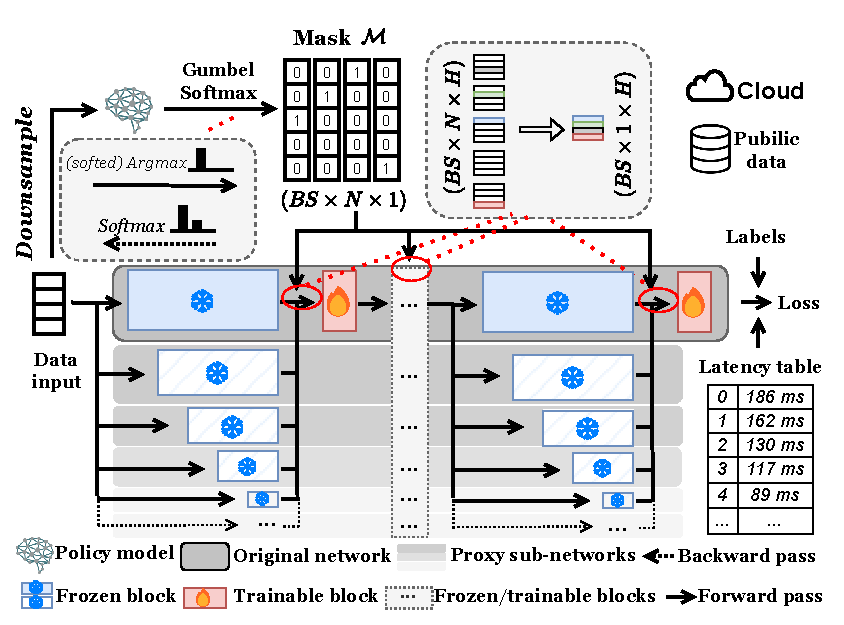
\includegraphics[width=0.98\linewidth]{figs/policy.pdf}
    \caption{Learning difficulty through joint training.}
    \label{fig:policy_model}
\end{figure}

\noindent \textbf{Joint training the policy model.}
The policy model is jointly trained with the original network and the proxy sub-networks (i.e., $\{\mathcal{F}_{n}\}, n \in \{0, 1, 2, \cdots, N\}$) on large-scale public cloud data.
% We pre-profile the proxy networks on device to obtain the realistic time consumption, and use the profiled latency during the policy model training.
The training procedure is shown in Figure ~\ref{fig:policy_model}.
We combine $\Omega$ and $\{\mathcal{F}_{n}\}$ together to create a joint end-to-end trainable network.
% Specifically, the manner in which we combine these networks is mainly demonstrated in Formula ~\ref{eq-policy_model_tuning_structure}.
The network structure before the $r_{th}$ trainable block (i.e., the red circle in Figure ~\ref{fig:policy_model}) is %can be represented by Equation ~\ref{eq-policy_model_tuning_structure}.
\begin{align}
	% y = sum(concat_{j=0}^{K}(x_{j}) \circ \mathcal{M}),
        x_{r} = \sum_{dim=1}[(x_{0}^{r}|x_{1}^{r}|\cdots|x_{n}^{r}|\cdots|x_{N}^{r}) \circ \mathcal{M}] 
	\label{eq-policy_model_tuning_structure}
\end{align}
% persudo code? formula is hard to express.
% squeeze?
where $x_{n}^{r} \in \mathbb{R}^{BS \times 1 \times H}$ is from the $n_{th}$ network $\mathcal{F}_{n}$, $\circ$ is the Hadamard product, $\mathcal{M} \in \mathbb{R}^{BS \times N \times 1}$ is the mask from the policy model, $BS$ is the mini-batch size, $N$ is the number of proxy sub-networks, $H$ is the hidden state size, $(x_{0}^{r}|x_{1}^{r}|\cdots|x_{n}^{r}|\cdots|x_{N}^{r})$ represents concatenating the tensors sequentially at the $1_{st}$ dimension, $\sum_{dim=1}$ represents summarizing the tensors along the $1_{st}$ dimension, and finally we get the input tensor $x_{r}$ of the $r_{th}$ trainable block.
% Each frozen block shares the input from the output of the previous block (usually the output of the preceding trainable block or the input to the entire model).
In addition, since the output of the policy model $\Omega$ is discrete, which makes $\Omega$ non-differentiable, we borrow the Gumbel-Softmax~~\cite{jang2017categorical} trick\footnote{An open-source implementation of Gumbel-Softmax Sampling: \url{https://github.com/gyhui14/spottune/blob/master/gumbel_softmax.py}} to facilitate the backpropagation of the gradient to the policy model.

We update the parameters of the policy model and the trainable blocks while keeping the frozen blocks frozen again.
We minimize a multi-task learning loss
% \begin{align}
% 	\mathcal{L} = -\sum_{i=1}^{k} y_i \log \left( \frac{e^{z_i}}{\sum_{j=1}^{k} e^{z_j}} \right) + \lambda \frac{1}{N}\sum_{*}(\mathcal{M} \circ \mathcal{S}),
% 	\label{eq-policy_model_tuning_loss}
% \end{align}

\begin{align}
	\mathcal{L} = \mathcal{L'} + \lambda \frac{1}{N}\sum_{*}(\mathcal{M} \circ \mathcal{S}),
	\label{eq-policy_model_tuning_loss}
\end{align}

where $\lambda$ is the scale factor (1.0 by default), $\sum_{*}$ represents summing all elements in the tensor, $\mathcal{M} \in \mathbb{R}^{N \times 1}$ is the mask tensor from the policy model, $\mathcal{S} \in \mathbb{R}^{N \times 1}$ is the on-device profiled latency scores of networks $\{\mathcal{F}_{n}\}$, $n \in \{0, 1, 2, \cdots, N\}$.
Equation ~\ref{eq-policy_model_tuning_loss} forces the policy model $\Omega$ to learn a strategy that minimizes computational complexity (the second term) while ensuring accuracy (the first term).

\noindent \textbf{Training data.}
\yws{
By default, the learning of policy model is on the large-scale general dataset used in the pre-training process (e.g. ImageNet).
Although the policy model is deployed on devices for new fine-tuning data, it shows a strong transferablity without the need for retraining the policy model in most cases, since a large-scale general training dataset has covered a wide range of difficulty patterns.
We make a detailed evaluation and discussion on the training data distribution issue in $\S$\ref{subsec: sensitivity} and $\S$\ref{subsec: discussion}.
}

% \mwx{Data distribution issue.}

\noindent \textbf{Training overhead.}
\yws{
The joint training converges within a single epoch and 
also only requires one-shot execution like the on-cloud pre-approximation.
In general, the entire training only incurs 5\%--10\% GPU-hours of the vanilla pre-training process.
}

% \subsection{Importance-based Data Skipping}
% \label{subsec:the importance filter}
% % \yws{(Shall we explain the difference between importance sampling (Mercury) and importance filtering?)}
% \mwx{This technique is not closely coupled with our key idea (proxy subnets), any idea?}
% \yws{Data importance influences routing strategy by feeding back to and modifying it. $\S$\ref{subsec:On-device training procedure} Policy\_sampler()}

% We use the feed-forward loss to estimate the importance $\mathcal{\psi}(x, t)$ of training data ~~\cite{mercury2021sensys, katharopoulos2017biased} during on-device training.
% The larger the loss, the more important the training data.
% \begin{figure}[!t]
    \centering
    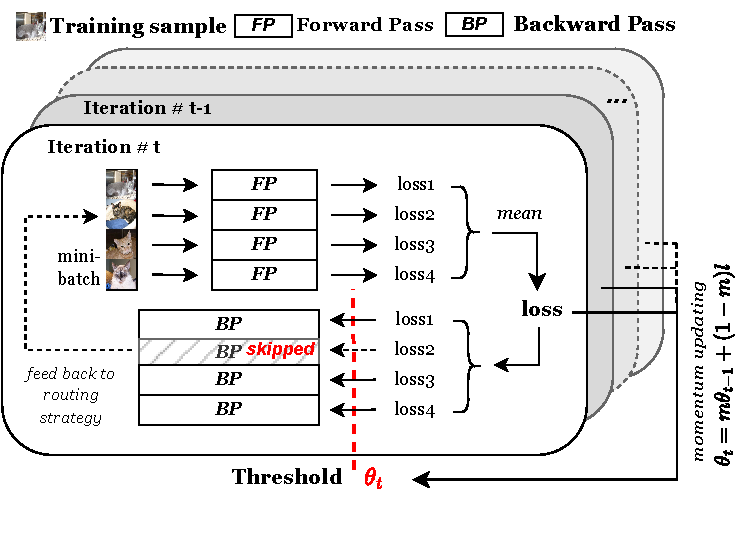
\includegraphics[width=0.82\linewidth]{figs/importance_filter.pdf}
    
    \caption{\sys opportunistic data skipping.}
    \label{fig:filter workflow}
    
\end{figure}

% \begin{figure}[!t]
    \centering
    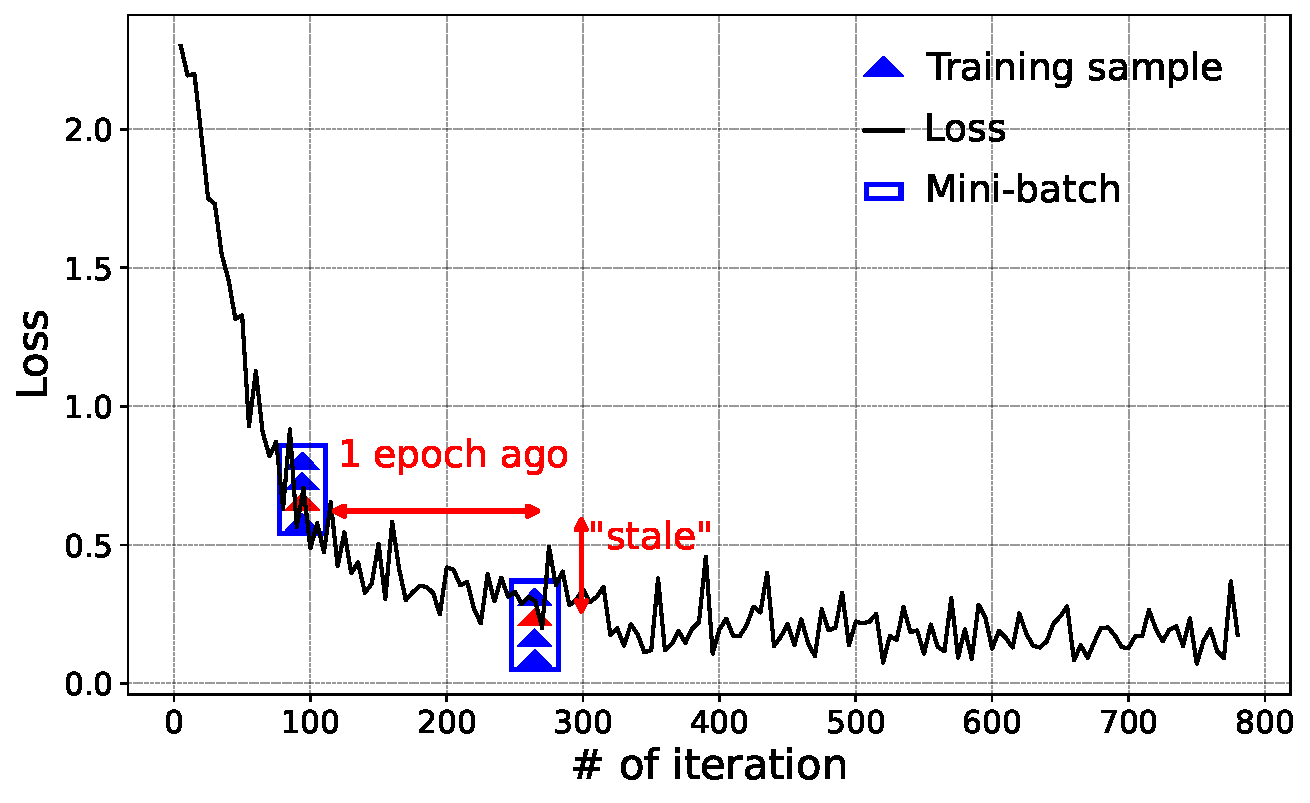
\includegraphics[width=0.82\linewidth]{figs/stale.pdf}
    \caption{The precision of data importance estimation. The estimate of specific training sample (red triangle) from the previous forward pass becomes ``stale'' as the training progresses.}
    \label{fig:stale}
\end{figure}


% \noindent \textbf{Challenges.}
% However, leveraging variations in data importance to expedite training convergence faces two challenges: (1) data importance estimation overhead; (2) precision of the estimation.
% On one hand, there are topological dependencies between various computational stages in a training iteration (Figure ~\ref{fig:filter workflow}). 
% To obtain the feed-forward loss, the forward pass must be performed first.
% On the other hand, since the NN weights are updated each training iteration, the estimation of data importance becomes ``stale'' over time (Figure ~\ref{fig:stale}).

% \noindent \textbf{Importance sampling approaches possess inherent limitations.}
% A feasible approach is to acquire the contemporaneous importance of all to-be-sampled training data before sampling the mini-batch, i.e., ``importance sampling'' ~~\cite{mercury2021sensys, katharopoulos2018not}.
% It inevitably imposes additional computational overhead associated with forward pass.
% \texttt{Mercury}\xspace ~~\cite{mercury2021sensys} hides this overhead by grouping and communication-computation overlapping, but it is difficult to perform this under our single-device setting.

% \noindent \textbf{The importance filter.}
% Therefore, we propose an importance filter to estimate $\mathcal{\psi}(x, t)$ only within the current iteration (Figure ~\ref{fig:filter workflow}).
% % The key idea behind the importance filter is simple: (1) It uses the loss obtained after the forward propagation in current iteration as an estimate of importance, thus avoiding the introduction of additional computational overhead; (2) 
% To perform stable and solid filtering, it decides whether the current data sample is filtered by comparing with a momentum updated threshold $\theta$.
% Let $\theta_{t}$ be the threshold at iteration $t$, $m\in[0, 1)$ be the momentum coefficient, $l$ be the loss of current iteration, then we get
% \begin{align}
% 	\theta_{t+1} = m\theta_{t} + (1-m)l.
% 	\label{eq-filter_thres}
% \end{align}
% Usually, $\theta$ is initialized as the loss from the first iteration, and $m$ is relatively large (e.g., 0.8, our default).
% We introduce a hyperparameter $\alpha$ to manually control the filtering strength, so the final filtering threshold is $\alpha\theta$. 
% % Please refer to the evaluation section ~\ref{} for detailed analysis.
% The backward pass and weight updating stages of the filtered samples will be skipped, and the routing strategy of these samples will be modified based on the feedback from the filter.

% % We also have to point out that when using on-device training frameworks with coarse-grained encapsulation, e.g., MNN, our importance filter can degrade to operate at the granularity of mini-batches rather than individual training samples. 
% % Due to the limited memory of edge devices using these frameworks, our filter still functions effectively with relatively small mini-batch sizes.

% \mwx{shall we emphasize that the skipping decision is dynamic across iterations? Use figures is necessary.}
% \yws{Maybe a behavior analysis in evaluation?}

% \subsection{The On-Device Training Controller}
% \label{subsec:On-device training procedure}
% % After describing how \sys minimizes the overhead of profiling data importance and data difficulty by using the policy model ($\S$\ref{subsec:the policy model}) and the importance filter ($\S$\ref{subsec:the importance filter}), let's put everything together and see how \sys performs on-device training.
% % \mwx{above sentence not needed?}
% We design a controller for \sys on-device training (Algorithm ~\ref{alg:on-device_training}).
% It receives \{$\mathcal{F}_{n}$\}, $\Omega$, $\alpha$, and the on-device dataset $D$, and finally outputs the fine-tuned network $\mathcal{F}_{0}$.
% \begin{algorithm}[t]
\scriptsize
\SetAlgoNlRelativeSize{-1}
% \SetAlgoNlRelativeSize{-3}
\SetAlgoNoEnd
\SetKwProg{Fn}{Function}{~}{end}
\SetKwInOut{Input}{input}\SetKwInOut{Output}{output}\SetKwInOut{Variable}{Variable}
\Input{\footnotesize
    \textcolor{blue!85!black}{$\{\mathcal{F}_{n}\}$}, $n \in \{0, 1, 2, \cdots, N\}$; \textcolor{blue!85!black}{$\Omega$}; On-device dataset \textcolor{blue!85!black}{$D$};
}
\Output{\footnotesize
    Fine-tuned \textcolor{blue!85!black}{$\mathcal{F}_{0}$};
}
\BlankLine
\Fn{\footnotesize \textcolor[RGB]{170,144,6}{data\_aware\_training():}}{
    % $loss\_func$ \textcolor{red!85!black}{$\leftarrow$} $CrELoss()$; 
    % \tcc{Initialization}
    \textcolor{blue!85!black}{$train\_loader$} \textcolor{red!85!black}{$\leftarrow$} \textcolor{blue!85!black}{$D$}, \textcolor[RGB]{170,144,6}{$Policy\_sampler()$};
    \textcolor{blue!85!black}{$\theta$} \textcolor{red!85!black}{$\leftarrow$} \textcolor{green!50!black}{$-1$}; 
    \textcolor{blue!85!black}{$m$} \textcolor{red!85!black}{$\leftarrow$} \textcolor{green!50!black}{$0.8$}\;
    \For{\textcolor{blue!85!black}{$epoch$} \textbf{in} \textcolor{blue!85!black}{$epochs$}}{
        \For{ \textcolor{blue!85!black}{$data$} \textbf{in} \textcolor{blue!85!black}{$train\_loader$}}{
            \textcolor{blue!85!black}{$X$}, \textcolor{blue!85!black}{$n$} \textcolor{red!85!black}{$\leftarrow$} \textcolor{blue!85!black}{$data$}; \textcolor{green!60!black}{\tcp{mini-batch and routing strategy}}
            \textcolor{blue!85!black}{$l$} \textcolor{red!85!black}{$\leftarrow$} \textcolor{blue!85!black}{$X$}, \textcolor{blue!85!black}{$\mathcal{F}_{n}$}; \textcolor{green!60!black}{\tcp{get loss by \textbf{one} sub-network $\mathcal{F}_{n}$}}
            \textcolor{green!60!black}{\tcc{Opportunistic data skipping}}
            \For{\textcolor{blue!85!black}{$x$} \textbf{in} \textcolor{blue!85!black}{$X$}}{
                \lIf{ \textcolor{blue!85!black}{$l[x]$} \textcolor{red!85!black}{>} \textcolor{blue!85!black}{$\theta$}}{
                    \textcolor{blue!85!black}{$l[x]$}\textcolor[RGB]{170,144,6}{$.bp()$};
                    \textcolor{blue!85!black}{$sampler$}\textcolor[RGB]{170,144,6}{.\textit{adjust}(}\textcolor{blue!85!black}{$x$}, \textcolor{green!50!black}{$0$}\textcolor[RGB]{170,144,6}{)}
                }\lElse{
                    \textcolor{blue!85!black}{$sampler$}\textcolor[RGB]{170,144,6}{.\textit{adjust}(}\textcolor{blue!85!black}{$x$}, \textcolor{green!50!black}{$1$}\textcolor[RGB]{170,144,6}{)}
                }
            } 
            \textcolor{green!60!black}{\tcc{Momentum-based filtering threshold}}
            \textbf{if} \textcolor{blue!85!black}{$\theta$}==\textcolor{green!50!black}{$-1$} \textbf{then} \textcolor{blue!85!black}{$\theta$} \textcolor{red!85!black}{$\leftarrow$} \textcolor{blue!85!black}{$l$}; \textbf{else} \textcolor{blue!85!black}{$\theta$} \textcolor{red!85!black}{$\leftarrow$} \textcolor{blue!85!black}{$m\theta$} + \textcolor{blue!85!black}{$(1-m)l$}\;
            \textcolor{green!60!black}{\tcc{Synchronizing trainable blocks}}
            \textbf{for} \textcolor{blue!85!black}{$i$} \textbf{in} \textcolor{blue!85!black}{\{0, 1, $\cdots$, $N$\}} \textbf{ do } \textcolor{blue!85!black}{$\ensuremath{\mathcal{F}_{i}}$} \textcolor{blue!85!black}{$.trainable$} \textcolor{red!85!black}{$\leftarrow$} \textcolor{blue!85!black}{$\ensuremath{\mathcal{F}_{n}}$} \textcolor{blue!85!black}{$.trainable$};
        }
    }
    \textbf{return} \textcolor{blue!85!black}{$\ensuremath{\mathcal{F}_{0}}$};
}
% \Fn{\footnotesize{\textcolor[RGB]{170,144,6}{Policy\_sampler():}} \scriptsize{\textcolor{green!60!black}{\tcp{called once per epoch}}}}{
%     aaa
% }

\Fn{\footnotesize{\textcolor[RGB]{170,144,6}{Policy\_sampler():}} \scriptsize{\textcolor{green!60!black}{\tcp*[h]{called once per epoch}}}}{
    \textcolor{blue!85!black}{$P$} \textcolor{red!85!black}{$\leftarrow$} \textcolor{blue!85!black}{$\Omega$}, \textcolor{blue!85!black}{$D$}; \textcolor{green!60!black}{\tcp{a list, routing strategy $n$ = $P$[index of $x$]}}
    \Fn{\footnotesize{\textcolor[RGB]{170,144,6}{adjust(\textcolor{blue!85!black}{$x$}, \textcolor{blue!85!black}{$\epsilon$})};} \scriptsize{\textcolor{green!60!black}{\tcp*[h]{adjust $x$'s routing strategy by $\epsilon$}}}}{}
    % $policy\_list$ \textcolor{red!85!black}{$\leftarrow$} adjust the $policy\_list$ based on the filter \; 
    \textcolor{blue!85!black}{$Q$} \textcolor{red!85!black}{$\leftarrow$} \textcolor{blue!85!black}{$[0:\textcolor[RGB]{170,144,6}{len(}D\textcolor[RGB]{170,144,6}{)}]$}; \textcolor{green!60!black}{\tcp*[h]{a list storing sampling order of $D$}} \\
    \textcolor{blue!85!black}{$Q$}\footnotesize{\textcolor[RGB]{170,144,6}{.\textit{sort}()}\textcolor[RGB]{170,144,6}{.\textit{shuffle}()}}; \scriptsize{\textcolor{green!60!black}{\tcp*[h]{sort by policy, shuffle in same policy}}} \\
    \textbf{return} \textcolor{blue!85!black}{$sampler$}; \textcolor{green!60!black}{\tcp*[h]{for $train\_loader$ to sample mini-batch}}
}

\caption{Data-aware on-device training.}
\label{alg:on-device_training}
\end{algorithm}

% The main body is shown in function $on\_device\_training\_controller()$.
% After some initialization (line 2), the controller performs the training loop (line 3--14).
% In each iteration, it samples a mini-batch $X$, obtains the routing strategy $n$, and selects a proxy sub-network $\mathcal{F}_{n}$ to calculate the loss (line 5--6).
% Please note that only \textit{one} proxy sub-network is involved in an on-device training iteration (unlike $\S$\ref{subsec:the policy model}), so keeping all proxy sub-networks in device memory simultaneously is not strictly necessary here.
% In line 7--12, the controller performs the importance-based data skipping ($\S$\ref{subsec:the importance filter}).
% It also synchronizes trainable blocks at the end of each iteration (line 13--14).

% In detail, the routing policy is maintained by the function $Policy\_sampler()$, which samples mini-batches for the $train\_loader$.
% Once per epoch, this function is called to obtain a difficulty-based routing strategy using the policy model $\Omega$ (line 17, $\S$\ref{subsec:the policy model}) and iteratively refine it based on feedback from the importance filter (line 18, line 8--10).

% Similar to a PyTorch sampler~\mwx{in design, better not mentioned specific libs}, \sys utilizes a $Policy\_sampler$ to comprehensively consider the difficulty and importance of training data for sampling before each epoch begins (line 3, 20-25). 
% In detail, each time the $Policy\_sampler$ is called, we compute the training dataset $D$ via the policy model $M_{p}$ to get the policy related to data difficulty. 
% After that, we adjust the policy based on the feedback of the importance filter, and sample training data with the same policy in each mini-batch. 
% This ensures that the same proxy network is used for training in each mini-batch, thus guaranteeing parallelism within the mini-batch and making efficient use of computational resources.

% The main body of the on-device training procedure is shown in function $on\_device\_training()$.
% Before starting the training loop, some initialization work needs to be performed first (line 2-4).
% The threshold $\theta$ and the momentum coefficient $m$ are initialized as -1 and 0.8 by default to guarantee a smooth estimation of the current convergence state during training.
% In the training loop (line 5-19), the $train\_loader$ returns a mini-batch of training data ($images$ and $labels$) and their selection policy ($idx$) for proxy networks.
% Then the selected proxy network $M_{idx}$ is used to perform the forward pass and calculate $curLoss$.
% The $curLoss$ is compared with the threshold $\alpha\theta$ to determine whether to continue with backward pass.
% If $curLoss > \alpha\theta$, then compute backward pass and keep the original policy for training data (line 10-12); otherwise, skip backward pass and adjust the policy of training data downwards (line 13-14), i.e., using a more lightweight proxy network.
% The threshold $\theta$ is updated with a momentum coefficient $m$ every mini-batch except for the initial one (line 15-18).
% At the end of a training loop, the trained parameters are updated from the current model to every proxy network (line 19).
% Online scheduling extension; matches the measured batch and feature schedulers.
\begingroup
\color{blue}
\subsection{Reordering Training Tasks for Co-Existing with Foreground Inference Tasks}
\label{subsec:reorder}

Different proxy networks take different amounts of time to process a batch.
When foreground inference runs periodically, background training must fit between requests.
FIFO waits if the next batch cannot finish in the remaining time, even when a later batch could fit.
Reorder uses this gap by running a suitable later task first.
It changes which task starts next; it does not interrupt a task that is already running.

\noindent\textbf{Choosing the next batch.}
Without feature caching, each task is a complete training batch.
Before starting one, we wait for any due foreground requests to finish.
We calculate the time left before the next request and subtract a small safety margin.
We first check the oldest waiting batch.
If its estimated runtime fits, we run it, just as FIFO would.
Otherwise, we look ahead through a limited number of waiting batches.
For each proxy, we consider only its earliest waiting batch, keeping batches for the same proxy in order.
Among the candidates that fit, we choose the one with the longest estimated runtime, using the earlier batch to break ties.
This aims to use as much of the gap as possible.
If no candidate fits, we wait and check again.

Figure~\ref{fig:reorder-example} shows three batches, A, B, and C, that use different proxies and need 15\,ms, 10\,ms, and 5\,ms, respectively.
The available training budget before foreground inference is 20\,ms.
Both methods first run A, leaving 5\,ms.
FIFO then waits because B cannot fit, whereas Reorder runs C in the remaining time.
After foreground inference, FIFO still needs to run B and C, while Reorder only needs to run B.
These durations illustrate the selection rule.

\begin{figure}[!t]
    \centering
    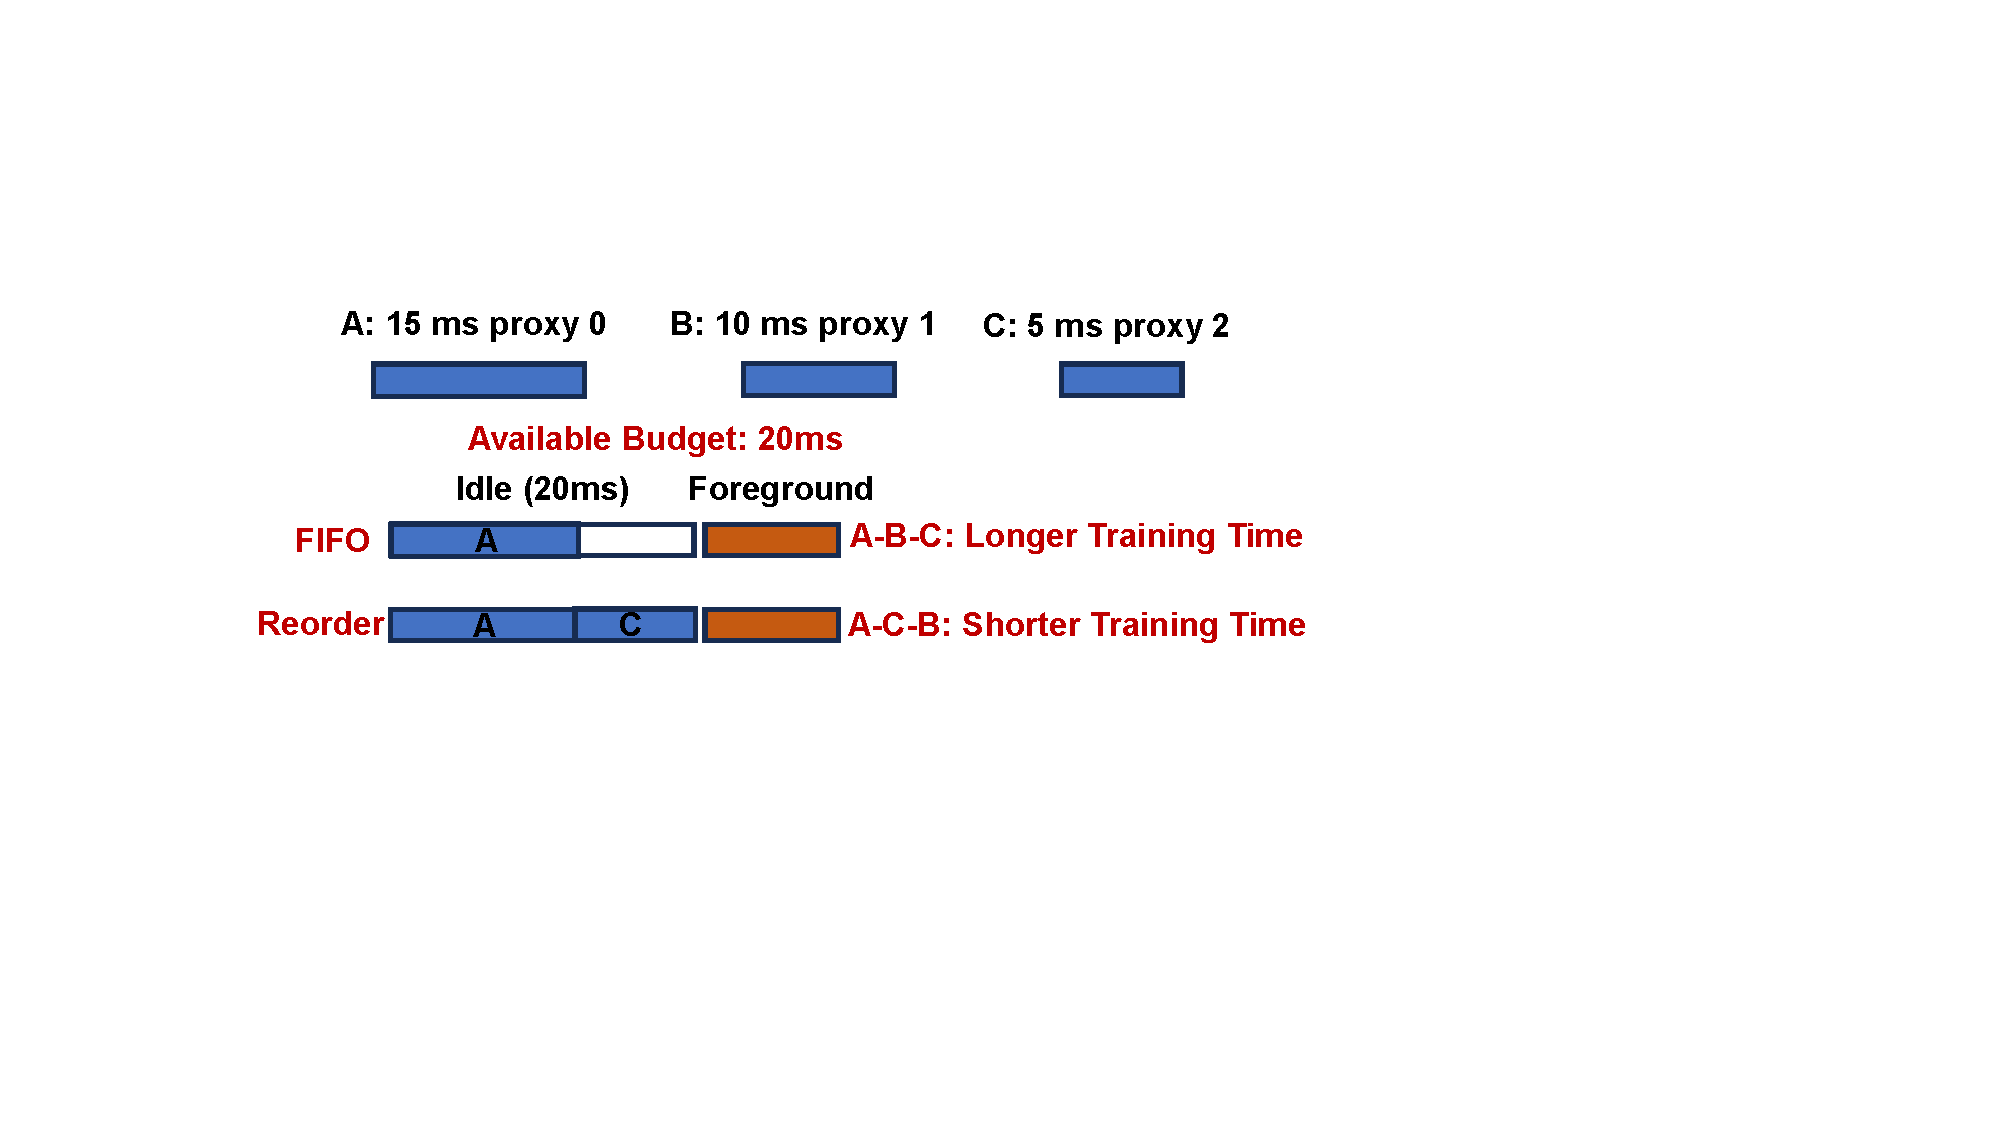
\includegraphics[width=0.98\columnwidth,pagebox=cropbox]{figures/reorder_piebridge.pdf}
    \caption{\textcolor{blue}{An example of FIFO and Reorder with a 20\,ms training budget between foreground inference requests. After A finishes, FIFO leaves 5\,ms unused because B cannot fit. Reorder uses this time to finish C, leaving less training work for the next window. Durations are illustrative.}}
    \label{fig:reorder-example}
\end{figure}

\noindent\textbf{Keeping batches from waiting too long.}
We count how often later batches run ahead of each waiting batch.
Once the oldest batch reaches a preset limit, we stop letting other batches pass it and wait until it fits.
Runtime estimates come from measurements and are updated as training proceeds.
For a complete training batch, the estimate reserves time for a full backward update before the loss-based decision is known.
Section~\ref{subsec:orin-periodic} gives the settings used in our experiments.

% Online-only extension; implementation and protocol in ../orin_scheduling/.
\begingroup
\color{blue}
\subsubsection{Feature Caching}
\label{subsec:feature-prefetch}

An idle gap between foreground requests may be too short for a complete training batch, but long enough for its frozen forward computation.
We cache the output just before the first trainable layer to schedule these two parts separately.
The frozen forward computation can finish in one gap, and training from the first trainable layer can resume in a later gap using the stored features.
We let each admitted operation finish without interrupting it.

The cache is a temporary buffer within one epoch.
It starts empty, and each feature is consumed once and then released.
The next epoch recomputes features even for the same sample and proxy.
Thus, caching does not remove forward computations through reuse across epochs; it allows their results to wait until the remaining training work can run.

Caching also allows us to prepare features for later batches.
For a fixed input and proxy, the frozen output does not depend on the current trainable parameters.
We can therefore reorder feature computations while keeping the work from the first trainable layer onward in the original batch order.
The original sampler sets the batch plan at the start of each epoch, and subsequent loss calculations, update decisions, and sampler feedback use the current parameters and loss history.

If the next batch's features are ready, its remaining training work takes priority; if that work cannot fit, we wait.
Otherwise, we first try to compute its missing features.
If they cannot fit, we look ahead and choose the longest fitting feature computation for another proxy.
We use a fixed-capacity buffer and reserve space for the earliest missing batch.
We admit each operation only when its estimated runtime fits before the next foreground request.
The cache stores features computed ahead of time, while Reorder chooses which ones to prepare.
Its scheduling benefit comes from using gaps that would otherwise be left idle.
Grouping batches that share a proxy can additionally improve forward efficiency, a benefit that does not require foreground inference.
Offline proxy generation and policy training stay unchanged.

\par
\endgroup

% Combined online loop, checked against prefetch_policy.py and
% prefetch_training_benchmark.py. The algorithm describes one training epoch.
\begingroup
\color{blue}
\subsubsection{Combining Feature Caching and Reordering}
\label{subsec:caching-reorder-algorithm}

Algorithm~\ref{alg:caching-reorder} combines the two designs for one epoch.
The original sampler provides the batch order and the proxy for each batch.
The cache $C$ holds features before the first trainable layer, indexed by batch ID; $i$ is the next batch whose remaining training work must run.
The cache starts empty in each epoch, while the trainable parameters and loss history carry over.

\textsc{TrainRest} runs from the first trainable layer using the current parameters.
It keeps the original loss-based update decision, EMA update, and sampler feedback in Algorithm~\ref{alg:on-device_training}.
Its runtime estimate reserves time for a full backward update.
\textsc{FrozenForward} computes only the frozen layers before this point and returns features for each original batch.
Both runtime estimates are updated after the corresponding operation finishes.

\begin{algorithm}[t]
\color{blue}
\footnotesize
\SetAlFnt{\footnotesize\color{blue}}
\SetAlCapFnt{\footnotesize\color{blue}}
\SetAlCapNameFnt{\footnotesize\color{blue}}
\SetNlSty{textbf}{}{}
\SetAlgoNlRelativeSize{-1}
\SetAlgoNoEnd
\SetKw{Continue}{continue}
\SetKwInOut{Input}{Input}
\Input{Ordered batches $Q=(X_j,y_j,p_j)_{j=1}^{M}$; cache capacity $K$ in batches; lookahead $L$; allowed group sizes $S$; safety margin $\delta$; runtime estimates}
\BlankLine
$C\gets\emptyset$; $i\gets 1$\;
\While{$i\le M$}{
    Wait until all due foreground requests finish\;
    $b\gets$ time until next request $-\delta$\;
    \If{$i\in C$}{
        \eIf{estimated runtime of \textnormal{\textsc{TrainRest}}$(i)\le b$}{
            \textsc{TrainRest}$(C[i],y_i,p_i)$\;
            Update its runtime estimate\;
            Release $C[i]$; $i\gets i+1$\;
        }{
            Wait briefly\;
        }
        \Continue\;
    }
    $\mathcal{G}\gets\emptyset$\;
    $W\gets$ uncached batches from $i$ to $\min(M,i+L-1)$\;
    \ForEach{proxy $p$ represented in $W$}{
        $J\gets$ batch IDs in $W$ using $p$, in order\;
        $r\gets K-|C|$\;
        \lIf{$i\notin J$}{$r\gets r-1$}
        $G\gets$ the longest prefix of $J$ with size in $S$, size $\le r$, and estimated forward time $\le b$\;
        \lIf{such a $G$ exists}{$\mathcal{G}\gets\mathcal{G}\cup\{G\}$}
    }
    \If{$\mathcal{G}=\emptyset$}{
        Wait briefly; \Continue\;
    }
    \eIf{a group in $\mathcal{G}$ contains $i$}{
        Select that group as $G$\;
    }{
        Select $G\in\mathcal{G}$ with the longest estimated forward time; break ties by earliest batch ID\;
    }
    $C[G]\gets\textsc{FrozenForward}(Q[G])$\;
    Update the forward runtime estimate for $G$\;
}
\caption{Feature caching with Reorder for one epoch.}
\label{alg:caching-reorder}
\end{algorithm}


When batch $i$ is cached, its remaining training work takes priority.
Otherwise, we prepare features for it if they fit, or use the gap for a later group.
Each group uses one proxy and takes the earliest uncached batches for that proxy within the lookahead range.
We keep the largest allowed group that fits both the time budget and the cache; a group that excludes $i$ must leave one cache slot free for it.
Only feature computation can move ahead: $i$ always advances in the original order, and each cached batch is released after use.
\par
\endgroup

\par
\endgroup

\section{Implementation and Methodology}
\label{sec:impl}

% 

\begin{table}[!t]
\caption{Datasets used in experiments. We report the number of training/testing samples separately in the column ``All''.}
\label{table-datasets}
\centering
\footnotesize
\begin{tabular}{@{}cccc@{}}
\toprule
\multirow{2}{*}{\textbf{Dataset}} & \multirow{2}{*}{\textbf{\# of Labels}} & \multicolumn{2}{c}{\textbf{\# of Samples}} \\ \cmidrule(l){3-4} 
                         &                              & Per-class     & All              \\ \midrule
Caltech-101~\cite{c101}              & 101                          & 40--800       & 3,060/6,084      \\
Caltech-256~\cite{c256}              & 257                          & 80            & 15,420/15,187    \\
Dogs vs. Cats~\cite{Dvg}            & 2                            & 900           & 1,800/2,000      \\
DTD~\cite{dtd}                      & 47                           & 120           & 3,760/1,880      \\ \bottomrule
\end{tabular}


\end{table}



\begin{table}[!t]
\caption{Details of devices used in the experiments.}
\label{table-hardware}
\centering
\scriptsize
\begin{tabular}{@{}l|l|l@{}}
\toprule
\textbf{Name}                                             & \textbf{Processor}                                                                                                                                   & \textbf{Software env.}                                                                            \\ \midrule
\begin{tabular}[c]{@{}l@{}}Jetson \\ TX2~\cite{tx2}\end{tabular}     & \begin{tabular}[c]{@{}l@{}}Dual-Core NVIDIA Denver 2 64-Bit CPU,\\ 256-core NVIDIA Pascal™ GPU.\end{tabular}                                         & \begin{tabular}[c]{@{}l@{}}Ubuntu 18.04 LTS, \\ PyTorch 1.7.1.\end{tabular}                      \\ \midrule
RPI 4B~\cite{rpi}                                                    & \begin{tabular}[c]{@{}l@{}}Broadcom BCM2711B0 quad-core \\ A72 64-bit @ 1.5GHz CPU.\end{tabular}                                                     & \begin{tabular}[c]{@{}l@{}}Raspbian 11,\\ PyTorch 1.7.1.\end{tabular}                              \\ \midrule
MI 10~\cite{mi10}                                                     & \begin{tabular}[c]{@{}l@{}}2.84GHz Cortex-X1, \\ 3× 2.4GHz Cortex A78, \\ 4× 1.8GHz Cortex A55 CPU.\end{tabular}                                     & \begin{tabular}[c]{@{}l@{}}Android 10, \\ MNN 2.0.0, \\ ONNX 1.13.1.\end{tabular} \\ \cmidrule(r){1-2}
\begin{tabular}[c]{@{}l@{}}Huawei \\ Mate 30~\cite{HuaWei}\end{tabular} & \begin{tabular}[c]{@{}l@{}}2x 2.86 GHz ARM Cortex-A76,\\ 2x 2.09 GHz ARM Cortex-A76,\\ 4x 1.86 GHz ARM Cortex-A55 CPU,\\ Kirin 990 NPU.\end{tabular} & \begin{tabular}[c]{@{}l@{}}Android 10, \\ MNN 2.0.0, \\ ONNX 1.13.1.\end{tabular} \\ \bottomrule
\end{tabular}



\end{table}

\begin{figure*}[!t]
  
    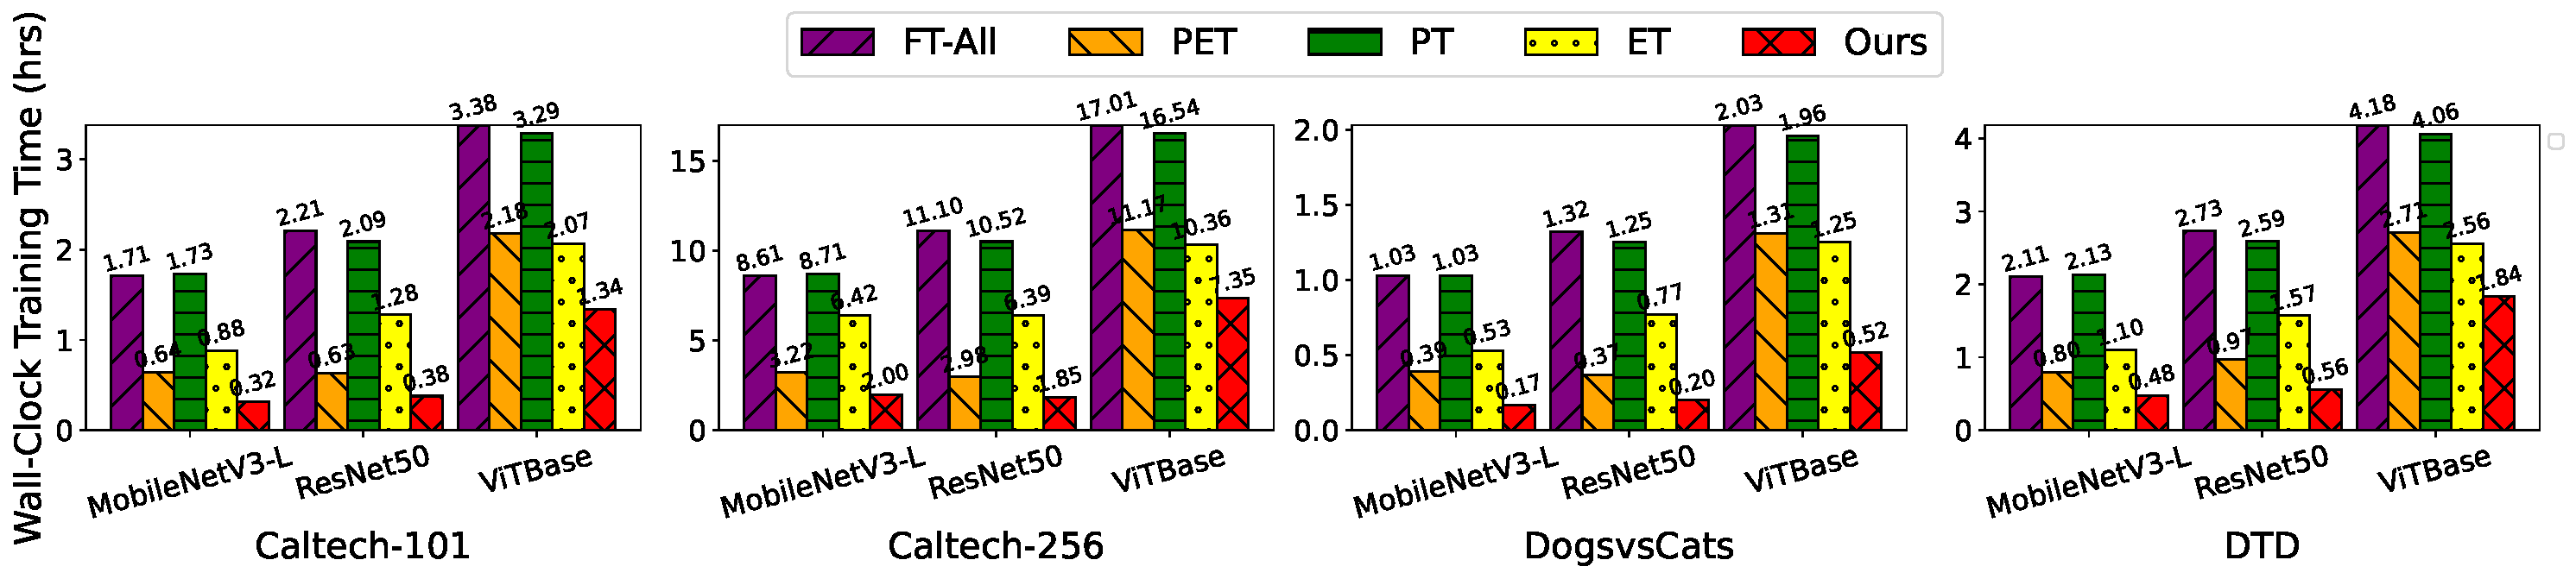
\includegraphics[width=0.97\textwidth]{figs/wallclocktime.pdf}

  \caption{Wall-clock on-device training time. Device: Jetson TX2.}
  
  \label{fig:e2etime}
\end{figure*}




\noindent \textbf{System implementation.}
We have fully implemented a \sys prototype with 4k LoC in Python and 3k LoC in C/C++ atop PyTorch and MNN~\cite{MNN}.
All the techniques of \sys can work in other ML frameworks designed for different devices and runtime environments like TensorFlow~\cite{tf} and TFLite~\cite{tflite}.
At the cloud side, we use a GPU server with 4× NVIDIA A40. 
At the edge side, we use devices described in Table ~\ref{table-hardware}.

% Both the NVIDIA Jetson TX2 and the Raspberry Pi 4B are widely used develop board on embedded platforms such as drones, smart cars and robots.
% Jetson TX2 is equipped with a Nvidia Pascal GPU with 256 CUDA cores, a 1.2GHz Cortex-A57 CPU and 8GB memory shared between GPU and CPU; Raspberry Pi 4B is equipped with a 1.5GHz Cortex-A72 CPU and 4GB memory.
% We also evaluate our system on a off-the-shelf smartphone MI10 which is equipped with a Snapdragon 865 SoC, and the experiments are run on CPU with 4 big cores.
% For Jetson TX2 and Raspberry Pi 4B, we use the Ubuntu 18.04 LTS OS with PyTorch 1.12.1;
% for MI10, we use the Android OS 10 with MNN 2.0.0 and ONNX 1.13.1.
% There are also several third-party libraries used at cloud pre-training stage, e.g., Once-For-All~\cite{} and Torch-Pruning~\cite{} for structural pruning and Pytorch Profiler~\cite{} and THOP~\cite{} for latency table profiling. 

\noindent \textbf{Models, datasets and metrics.}
% \mwx{have a table for models and datasets}
We evaluate \sys with the following representative models: MobileNetV3-L~\cite{howard2019searching}, ResNet50~\cite{he2015deep} and ViT\_base~\cite{dosovitskiy2021an}.
% These models encompass various architectures, computational costs, and capacities, and are specified with different trainable components during on-device fine-tuning.
% For MobileNetV3, we fine-tune only the head; for ResNet50, we fine-tune the head and an adapter; for VIT base, we fine-tune the head and 6 adapters. 
% All the adapters used in each model have the same latent size and are inserted layer by layer starting from the model’s output layer moving forward.
We on-cloud pre-train these models with the ImageNet2012~\cite{ImageNet2012} dataset that contains 1.2M images, and then on-device fine-tune them with the downstream datasets (Caltech-101~\cite{c101}, Caltech-256~\cite{c256}, Dogs vs. Cats~\cite{Dvg}, DTD~\cite{dtd}) which are more fine-grained.
We mainly focus on the following metrics: \textit{the wall-clock on-device training time} and \textit{the best test accuracy}.
% \begin{itemize}[leftmargin=*]
% \item \textbf{Caltech-101} with 3,060 training data and 6,084 testing data. 
% It contains 101 long-tailed distributed categories of images, with approximately 40 to 800 images per category, including common objects such as animals and vehicles.    

% \item \textbf{Caltech-256} with 15,420 training data and 15,187 testing data, which is 
% an extended version of Caltech-101, with more complicated classification categories and similarly fewer samples per category (80 in average).

% \item \textbf{Dogs vs. Cats} with 25,000 images of dogs and cats.
% It is relatively simple but serves as a very classic benchmark dataset for evaluating transfer learning performance in downstream tasks.
% We sample a subset of 1,800 training data and 2,000 testing data from the parent dataset, with an equal number of cats and dogs.

% \item \textbf{DTD} with 3,760 training data and 1,880 testing data.
% Unlike the previous datasets, the DTD (Describable Textures Dataset) contains 47 different categories of texture images. 
% These texture categories include various materials, object surfaces, and natural textures such as grass, bark, water, fabric, brick walls, and more. 
% Each texture category consists of approximately 120 images.
% \end{itemize}



\begin{table*}[!t]
\caption{Accuracy of \sys and baselines. C-101: Caltech-101; C-256: Caltech-256; DVC: Dogs vs. Cats.}
\label{table-e2e accuracy}
\centering

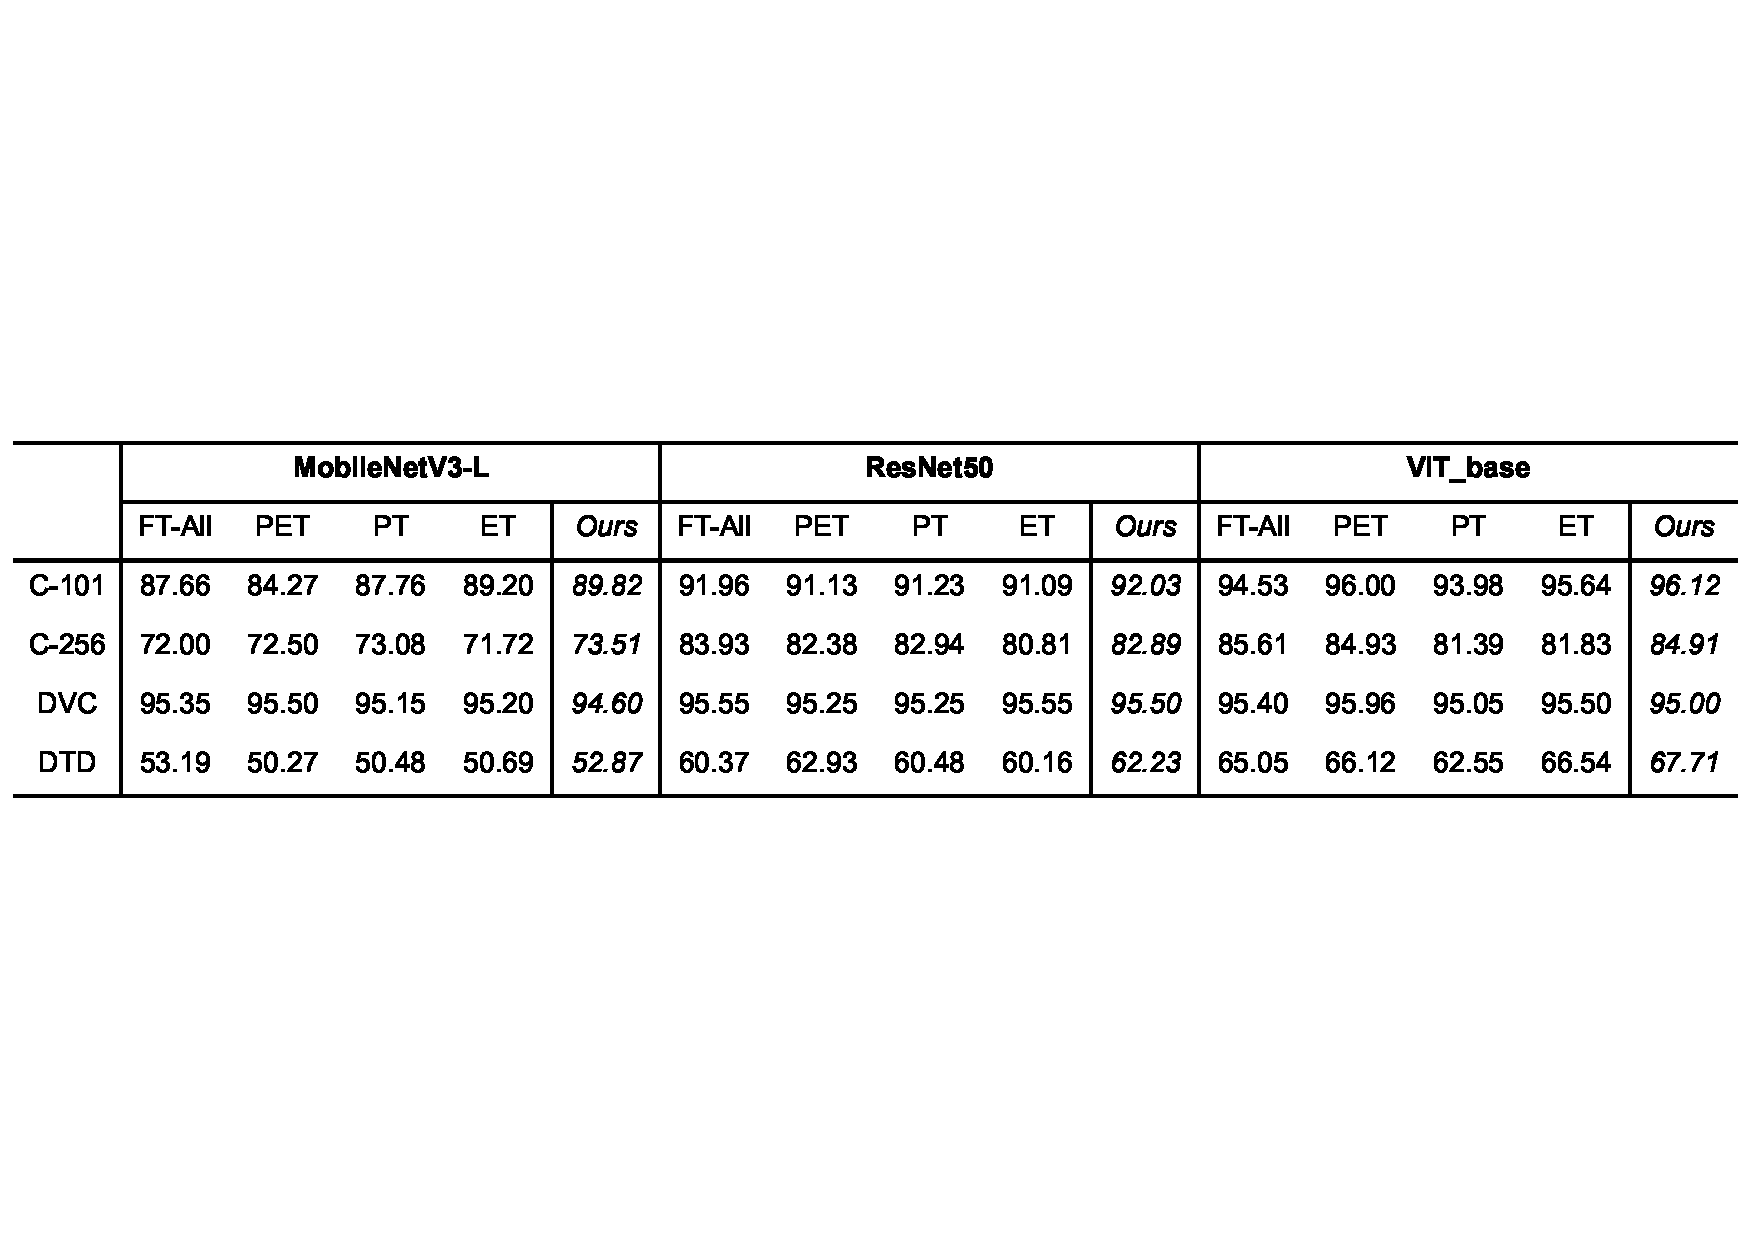
\includegraphics[width=0.80\textwidth]{figs/dynaproxyer_acc.pdf}




\end{table*}


\noindent \textbf{Baselines.}
We compare \sys to these alternatives:
% \begin{itemize}[leftmargin=10pt, topsep=0pt]
Fine-tuning all parameters (\texttt{FT-All}) always fine-tunes the whole pre-trained NN. This is the default fine-tuning methodology used in most pre-training-and-fine-tuning paradigms.
Parameter-Efficient Training (\texttt{PET}) freezes most layers of the pre-trained NN and trains only a small portion. We evaluate various PET methods: Linear Probing~\cite{kumar2022finetuning} for ResNet50, Last-3~\cite{guo2019spottune, MLSYS2019_e09d45e1} for MobileNetV3 and Adapters(12)~\cite{rebuffi2017learning, houlsby2019parameter} for ViT\_base.
PruneTrain (\texttt{PT})~\cite{10.1145/3295500.3356156} is a framework that dynamically prunes the NN during training. %It profiles the importance of channels at runtime and gradually removes less important channels to reduce the end-to-end training time.
ElasticTrainer (\texttt{ET})~\cite{huang2023elastictrainer} is one of the state-of-the-art on-device training frameworks that dynamically determines trainable layers by estimating the importance of NN tensors.

\noindent \textbf{Hyper-parameters.}
% We empirically use the following hyper-parameters:
The momentum coefficient $m$ of PruneTrain is 0.8.
% The pruning step $d$ is 10\%. 
% The number of proxy networks is 10.
The L1 penalty coefficient of PruneTrain is set to 1e-4.
The ratio $\rho$ of ElasticTrainer is set to 0.4.
To provide big-enough search space, we on-cloud generate $N=10$ proxy sub-networks with a pruning step size $d=7\%$--$10\%$. 
Limited by the memory constraint of edge devices, the mini-batch size is set to 4.
Training epochs are set to 12 following prior work ~\cite{huang2023elastictrainer}.
% The learning rate is 1e-4. 
% The optimizer is standard SGD.
Training samples are resized to a 224$\times$224 RGB image with standard data augmentation strategies such as random cropping and flipping.



\begin{figure}[!t]
	\centering
	\subfloat[Time to accuracy\label{fig:time2acc}]{%
  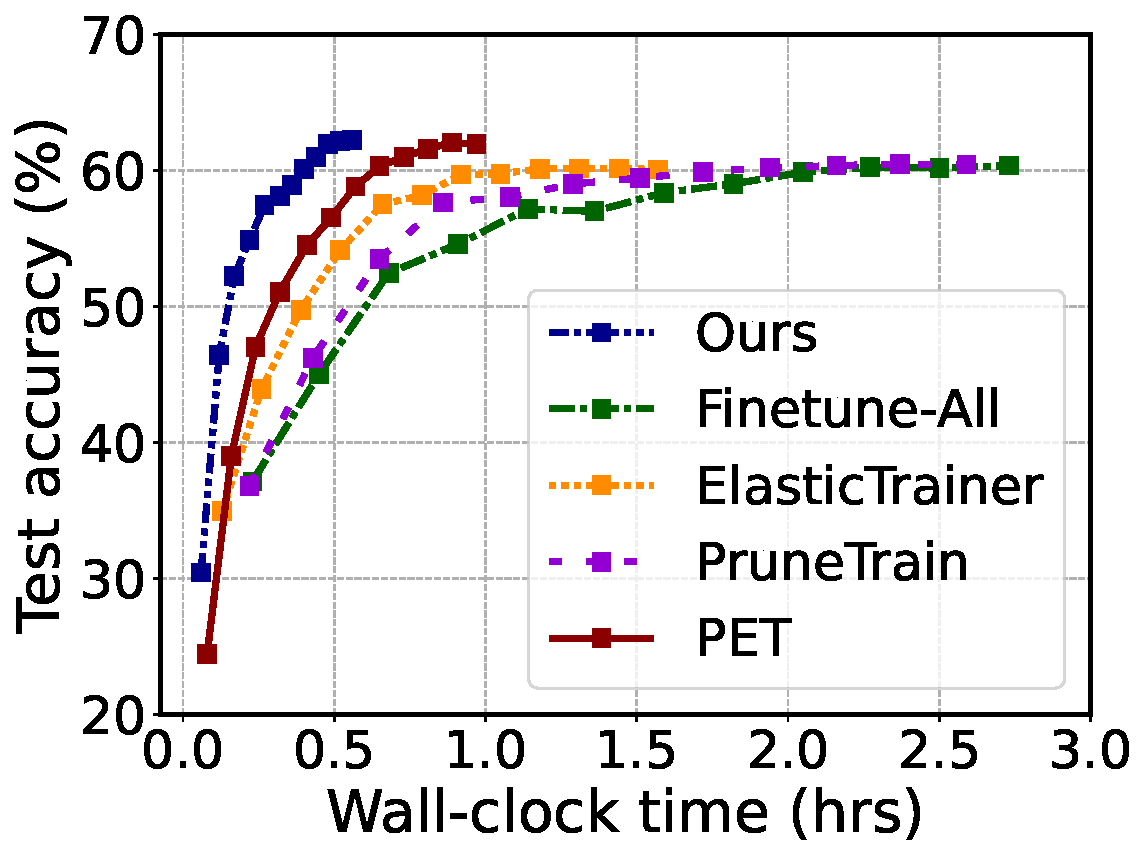
\includegraphics[width=0.55\linewidth]{figs/time2acc.pdf}}
        \hfill
	\subfloat[Speedup\label{fig:speedup2acc}]{%
  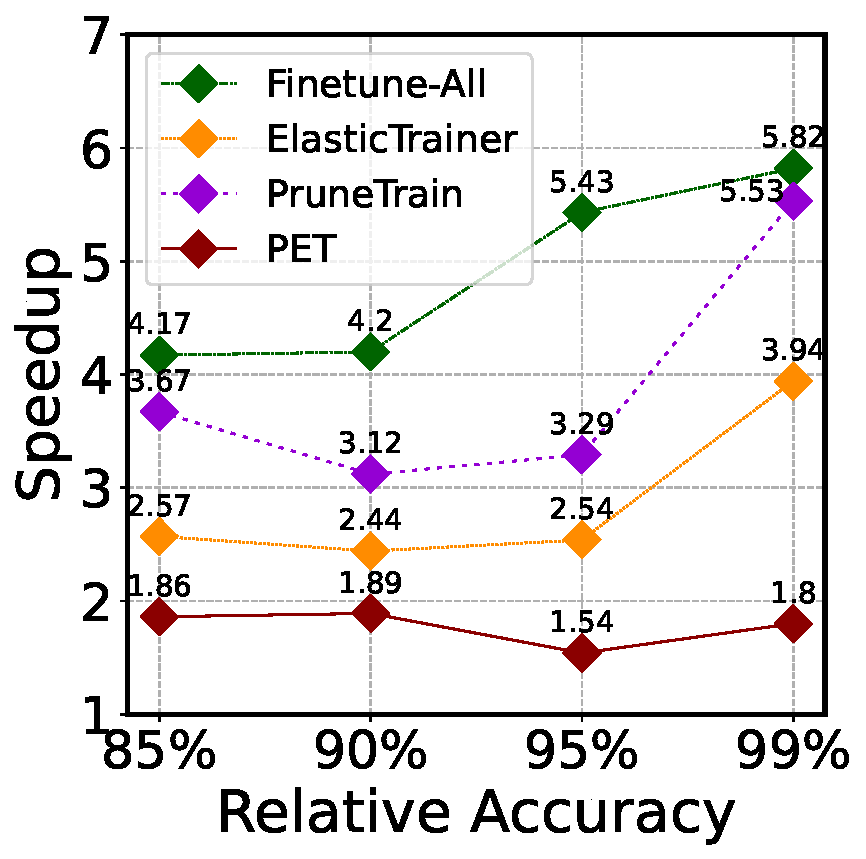
\includegraphics[width=0.43\linewidth]{figs/speedup2acc.pdf}}
        
	\caption{\sys achieves significant speedup across different accuracy targets. Model: ResNet50; Dataset: DTD.}
        
        \label{targeted acc}
\end{figure}

\section{Evaluation}
\subsection{End-to-End Performance}
% In this section, we mainly compare the wall-clock on-device training time and the test accuracy of \sys to baselines under various models, datasets and devices.

% \noindent \textbf{\sys reduces on-device training time significantly without compromising the test accuracy.}
\noindent \textbf{Overall performance.}
We begin with comparing the overall performace of \sys to its baselines.
We conduct the experiments on 3 various NN architectures and 4 various downstream datasets. 
The details are mentioned in $\S$\ref{sec:impl}.
We record the test accuracy every epoch and report the best test accuracy and corresponding wall-clock training time.
The computing cost on testing is excluded.
Table ~\ref{table-e2e accuracy} shows the best test accuracy.
\sys does not compromise test accuracy compared to its baselines.
As is shown in Figure ~\ref{fig:e2etime}, by dynamically routing training data to lightweight subnets, \sys achieves up to 6.60$\times$ speedup over all baselines, and 1.47$\times$--2.52$\times$ speedup compared to \texttt{PET}. 
% Specifically, \sys achieves 
Here we perform a detailed analysis:
\begin{itemize}[leftmargin=10pt,topsep=0pt]
\item \textit{Compared to \texttt{FT-All}.}
\sys significantly outperforms \texttt{FT-All} by up to 6$\times$.
This comes from both the parameter efficiency and our key designs.
\item \textit{Compared to \texttt{PET}.}
\sys consistently outperforms \texttt{PET} by up to 2.5$\times$.
This is attributed to the full utilization of data diversity.
\item \textit{Compared to other strong baselines (\texttt{PT}/\texttt{ET}).}
\sys also outperforms these strong baselines.
\texttt{PT}'s NN approximation only reduces training FLOPs, which does not translate to wall-clock time reduction on general-purpose processors.
\texttt{ET} only performs tensor-level non-deterministic training with evaluated importance. It cannot fully utilize the potential of NN approximation and data diversity.
Another significant drawback is that they compromise parameter efficiency, preventing them from enjoying various benefits of PET in terms of both training and deployment mentioned in $\S$\ref{subsec:PET}.
\end{itemize}

% \noindent $\bullet$ \textit{\sys v.s. FT-All/PT/ET.}
% FT-All is time-consuming without parameter-efficiency and NN approximation.
% PT online approximates the network during on-device training but with extra pruning overhead.
% % It achieves similar performance to FT-All.
% ET only partially benefits from parameter-efficiency.
% Therefore, \sys can achieve significant improvements (up to 6.1$\times$/6.6$\times$/3.9$\times$ on 3 networks with various PET methods) compared to these baselines.

% \noindent $\bullet$ \textit{\sys v.s. PET.}
% \sys outperforms PET by 1.47$\times$--2.52$\times$.
% These numbers come from NN approximation of \sys, and are influenced by PET settings.


\noindent \textbf{Performance under various accuracy budgets. }
In practice, on-device training tasks often do not choose to reach the highest test accuracy because of the marginal effect.
Thus, we also explore the wall-clock training time for different accuracy targets.
Figure ~\ref{fig:time2acc} shows the time-to-accuracy curve of \sys and its baselines.
We observe that, thanks to our dynamic routing design, \sys achieves shorter per-epoch computation time and faster end-to-end convergence speed.
Further, we report the speedup achieved by \sys when reaching 85\%/90\%/95\%/99\% of the baseline's best accuracy.
As is shown in Figure ~\ref{fig:speedup2acc}, \sys always achieves significant speedup (1.86$\times$/1.89$\times$/1.54$\times$/1.80$\times$ to \texttt{PET}, and 4.17$\times$/4.20$\times$/5.43$\times$/5.82$\times$ to \texttt{FT-All}) under different accuracy budges.
Specifically, there is a trend that the higher the target accuracy, the greater the speedup achieved by \sys.
This is because, as training progresses, more and more data require fewer computational resources, allowing \sys to effectively mitigate the marginal effect of training.

\noindent \textbf{Performance on various devices.}
We further explore the performance of \sys on 3 devices: Jetson TX2, Raspberry Pi 4B and MI 10 smartphone in Figure ~\ref{fig:crossdevice}.
\sys outperforms its baselines on all these devices by a minimum factor of 1.61$\times$/1.63$\times$/1.72$\times$, and the improvements are particularly notable on both GPU-empowered devices (e.g., Jetson TX2) and resource-constrained devices (e.g., Raspberry Pi 4B and MI 10 smartphone).

\noindent \textbf{Performance in extremely few-shot scenarios.}
We also explore the performance of \sys with extremely few human-labeled training data in Table \ref{table-fewshot}. 
Our system consistently outperforms the baseline method under 5-shot/10-shot settings.
We further apply a commonly used few-shot learning approach: pseudo-labeling~\cite{lee2013pseudo}. 
We provide 100 pseudo-labeled data for each category. 
\sys significantly outperforms the baseline and achieves accuracy close to training with adequate human-labeled data.

% Specifically, \sys is friendly to AI accelerators (NPUs) designed for NN inference, making on-device fine-tuning practical and even efficient.
\begin{table}[!t]
\caption{Performance in extremely few-shot scenarios. PL: Pseudo Labeling; Model: ResNet50; Dataset: DTD Device: Jetson TX2.}
\label{table-fewshot}
\centering
\footnotesize
\begin{tabular}{@{}ccccccc@{}}
\toprule
                     & \multicolumn{3}{c}{\textbf{FT-All}} & \multicolumn{3}{c}{\textbf{\sys}} \\ \cmidrule(l){2-7} 
                     & 5-shot      & 10-shot     & PL      & 5-shot     & 10-shot     & PL     \\ \midrule
\textbf{Time (min.)} & 7.92          & 16.38          & 138.21     & 3.60         & 5.97          & 35.53    \\
\textbf{Accu. (\%)}   & 12.92          & 27.28          & 55.32      & 18.13         & 32.71          & 60.15     \\ \bottomrule
\end{tabular}
    
    
    
\end{table}

\begin{figure}[!t]
    \centering
    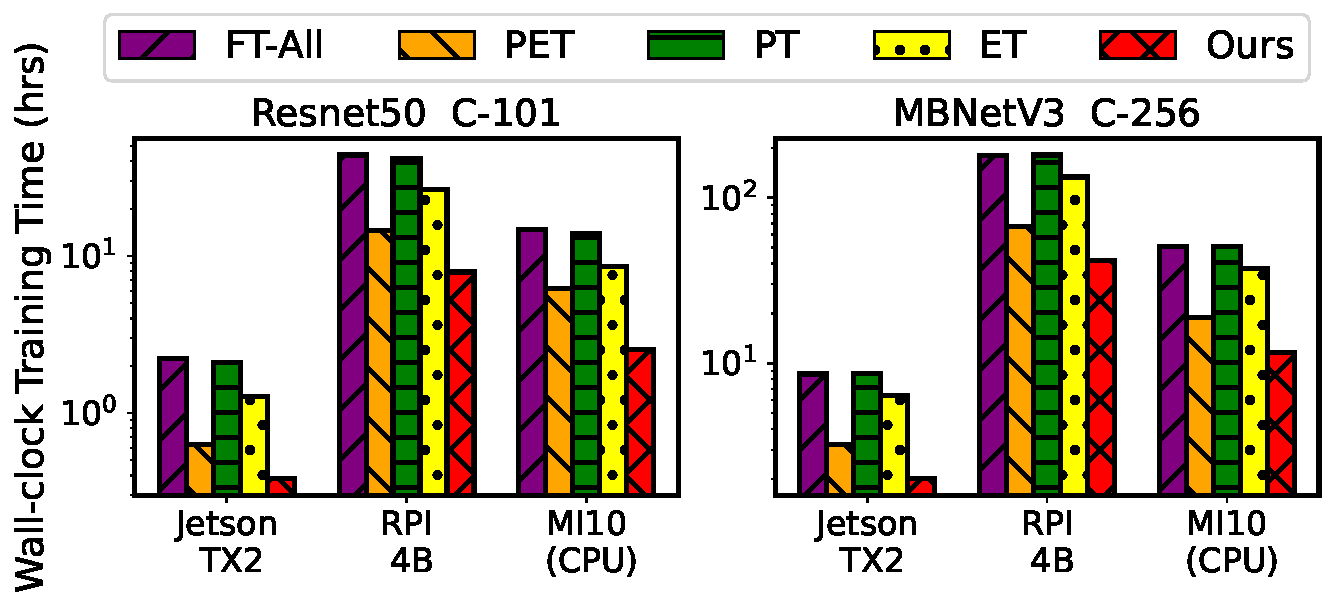
\includegraphics[width=0.96\linewidth]{figs/cross_devices.pdf}
    
    \caption{Performance on various devices.}
    
    \label{fig:crossdevice}
\end{figure}


\begin{figure}[!t]
    \centering
    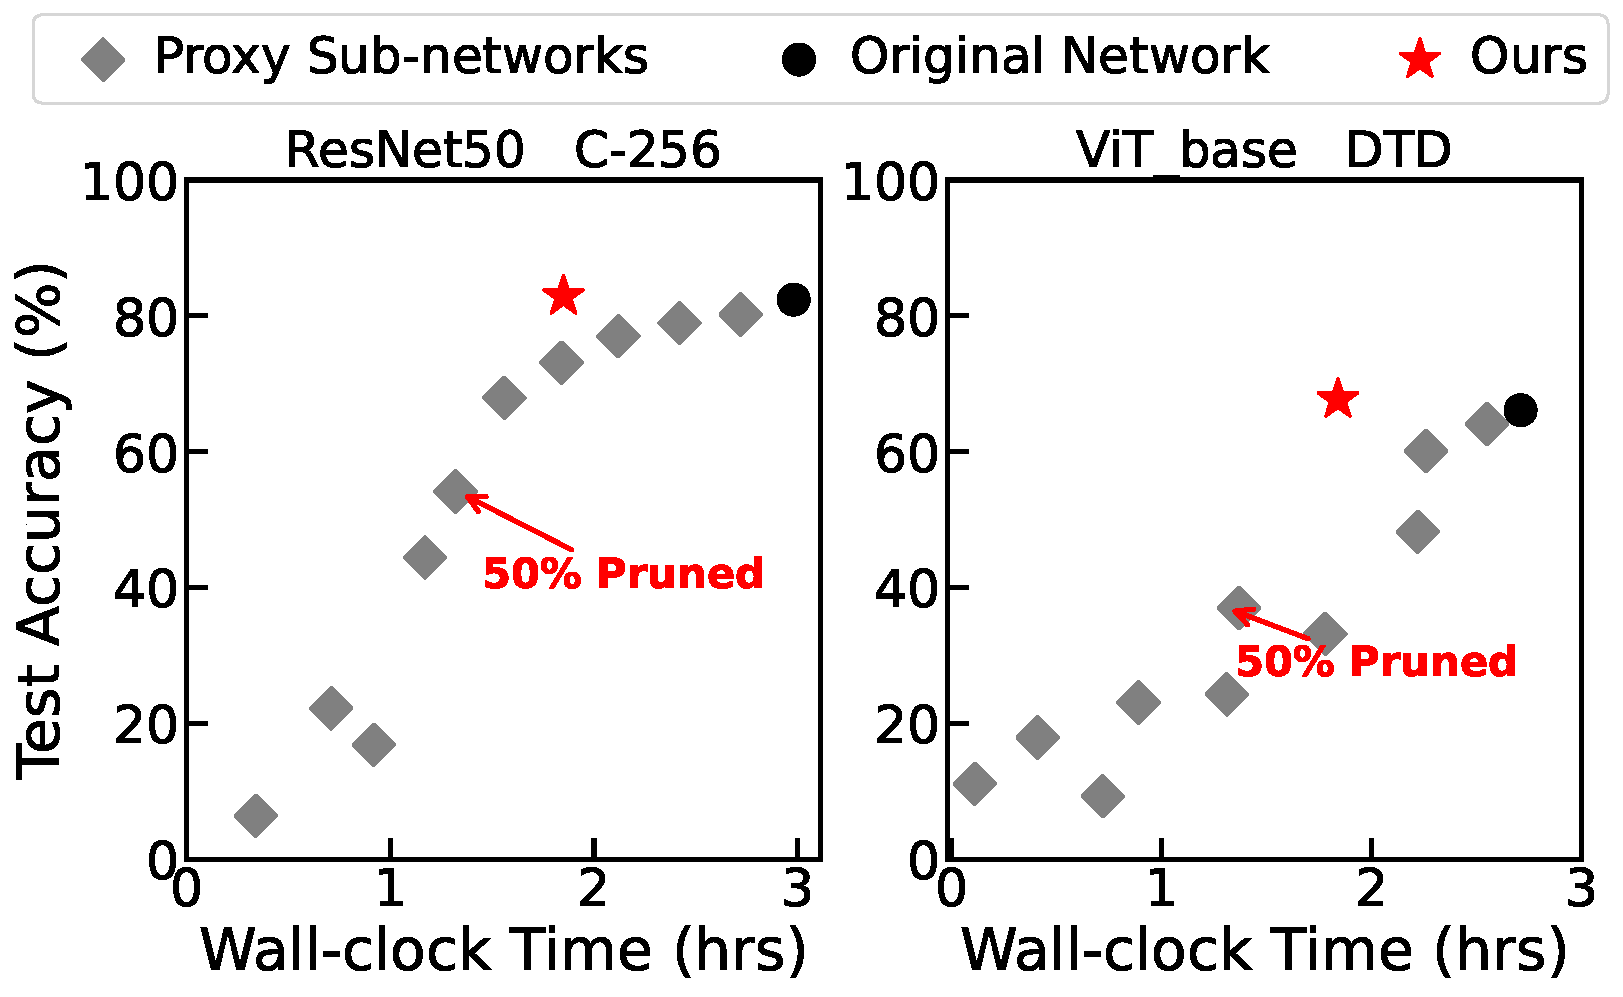
\includegraphics[width=0.76\linewidth]{figs/static.pdf}
    
    \caption{Compared to static alternative proxy sub-networks. Our data-aware subnet routing is a pareto-improved solution.}
    
    \label{fig:static}
\end{figure}



% \label{subsec:ablation}

\subsection{Design Effectiveness and Sensitivity Analysis}
\label{subsec: sensitivity}
In this section, our primary focus is on analyzing the effectiveness and sensitivity of \sys design.

\noindent \textbf{Compared to static alternative proxy sub-networks.}
We compare our data-aware subnet routing strategy ($\S$\ref{subsec:data-aware training}) to statically routing all training samples to the same proxy sub-network.
Figure ~\ref{fig:static} shows the best test accuracy and wall-clock training time of the original network ($\bullet$), the proxy sub-networks (\textcolor{gray}{\scriptsize $\blacklozenge$}) and our data-aware subnet routing (\textcolor{red}{$\star$}).
We have the following observations:

(1) \textit{A simple, static replacement strategy could result in nontrivial degradation of convergence accuracy.}
% As proxy sub-networks become lighter, their test accuracy rapidly decreases.
After pruning the original network by 50\%, ResNet50 experiences a 28.24\% decrease in test accuracy on the Caltech-256 dataset, and ViT\_base suffers a 29.11\% decrease in test accuracy on the DTD dataset.
There are two reasons behind this. 
One is that there is an error between the original network and the approximated subnet. 
The other is that, without a resource-intensive search, the pruned network structure may not be optimal.

\begin{figure}[!t]
    \centering
    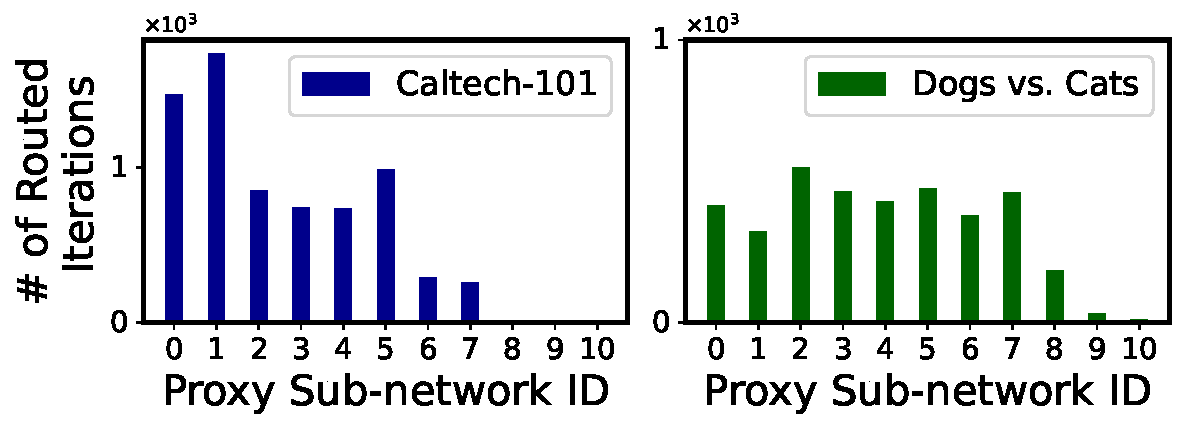
\includegraphics[width=0.82\linewidth]{figs/behavior.pdf}
    
    \caption{Behavior on datasets of different complexity.}
    
    \label{fig:behavior}
\end{figure}


(2) \textit{Our data-aware subnet routing is a pareto-improved solution.}
Compared to other static solutions, our approach not only reduces training time but also does not exhibit a noticeable decrease in accuracy.

\noindent \textbf{Behavior on datasets of different complexity.}
As is shown in Figure ~\ref{fig:behavior}, compared to the more complex dataset Caltech-101, \sys effectively routes more training samples to lighter subnets on Dogs vs. Cats dataset.

\noindent \textbf{Number of proxy sub-networks.}
Recall that we globally choose a proxy number $N$ = 10 (the pruning step size $d$ is about $1/N$).
Here we analysis the rationale and influence of choosing this factor.
As shown in Figure~\ref{fig:sensitivity}(a), a larger N provides more fine-grained approximation tradeoffs, but its benefit diminishes when large enough (e.g., >=10). 
Determining it properly isn't a challenge: \sys can provide heuristic suggestions to a typical range (e.g., 10--15); or the cloud can automatically obtain it through profiling on public dataset.

From our observation, the number of subnets does not apparently influence wall-clock training time (Figure~\ref{fig:sensitivity}(b), ResNet50+Caltech-256+TX2).
This is mainly because the size of the subnets already covers the entire trade-off space, regardless of the number $N$.

\noindent \textbf{Policy model training data.}
% \mwx{Add more explanations. In general, (1) data diversity is common characteristics that is more transferable. (2) large scale pretraining is the best way to capture this characteristic. (3) a severe OOD issue can be addressed by crowd-sourcing a portion of trainable data, federated learning the policy model or directly on-device continual training the policy model.}
\yws{
Recall that we train our policy model $\Omega$ on large scale public dataset, i.e. ImageNet.
Through the aforementioned end-to-end experiments, its effectiveness has been verified.
Here we discuss \sys's sensitivity to the data for capturing data difficulty.
We report fine-tuning ResNet50 on Caltech-101 dataset.
The data difficulty learned from the large-scale general dataset ImageNet exhibits a strong \textit{transferability}.
Figure~\ref{fig:sensitivity}(c) shows that training on ImageNet achieves comparable accuracy compared to directly training on Caltech-101.
When training policy model with 5\% data (simulating crowd-sourcing user-permitted training data), the policy model still can work well.
Only when the cloud training data completely mismatches with device data (e.g., using cifar-10 for training in Figure~\ref{fig:sensitivity}(c)), the policy model behaves biased.
}

\begin{table}[!t]
\caption{\yws{Significance of key designs.}}
\label{table:ablation}
\centering
\footnotesize
\setlength{\tabcolsep}{3pt}
\begin{tabular}{@{}L{0.42\linewidth}C{0.25\linewidth}C{0.25\linewidth}@{}}
\toprule
\textbf{Design} & \textbf{Training Time (h)} & \textbf{Test Acc. (\%)} \\
\midrule
\sys & 1.85 & 82.89 \\
W/O IDC pruning & N/A (shape mismatch) & N/A (shape mismatch) \\
W/O latent space alignment & 2.06 & 64.24 \\
W/O policy model based routing & 26.2 & 82.62 \\
\bottomrule
\end{tabular}
\end{table}

\noindent \textbf{Significance of key designs.}
% \mwx{IDC pruning, latent space alignment. has been discussed before. but make a summarization here.}
\yws{
In Table~\ref{table:ablation}, we show the significance of \sys's key designs.
We report fine-tuning ResNet50 on Caltech-256, Jetson TX2.
The results show that without IDC pruning, the proxy subnets cannot replace the original network because of shape mismatch.
Without latent space alignment, the pruned subnets conflict with each other, leading to a significantly dropped convergence accuracy.
Without the lightweight policy model for perceiving the data difficulty, the training is slowed down by over 13$\times$, because that \sys has to run each subnet to get and compare the extracted feature in each iteration.
}
\begin{figure}[!t]
    \centering
    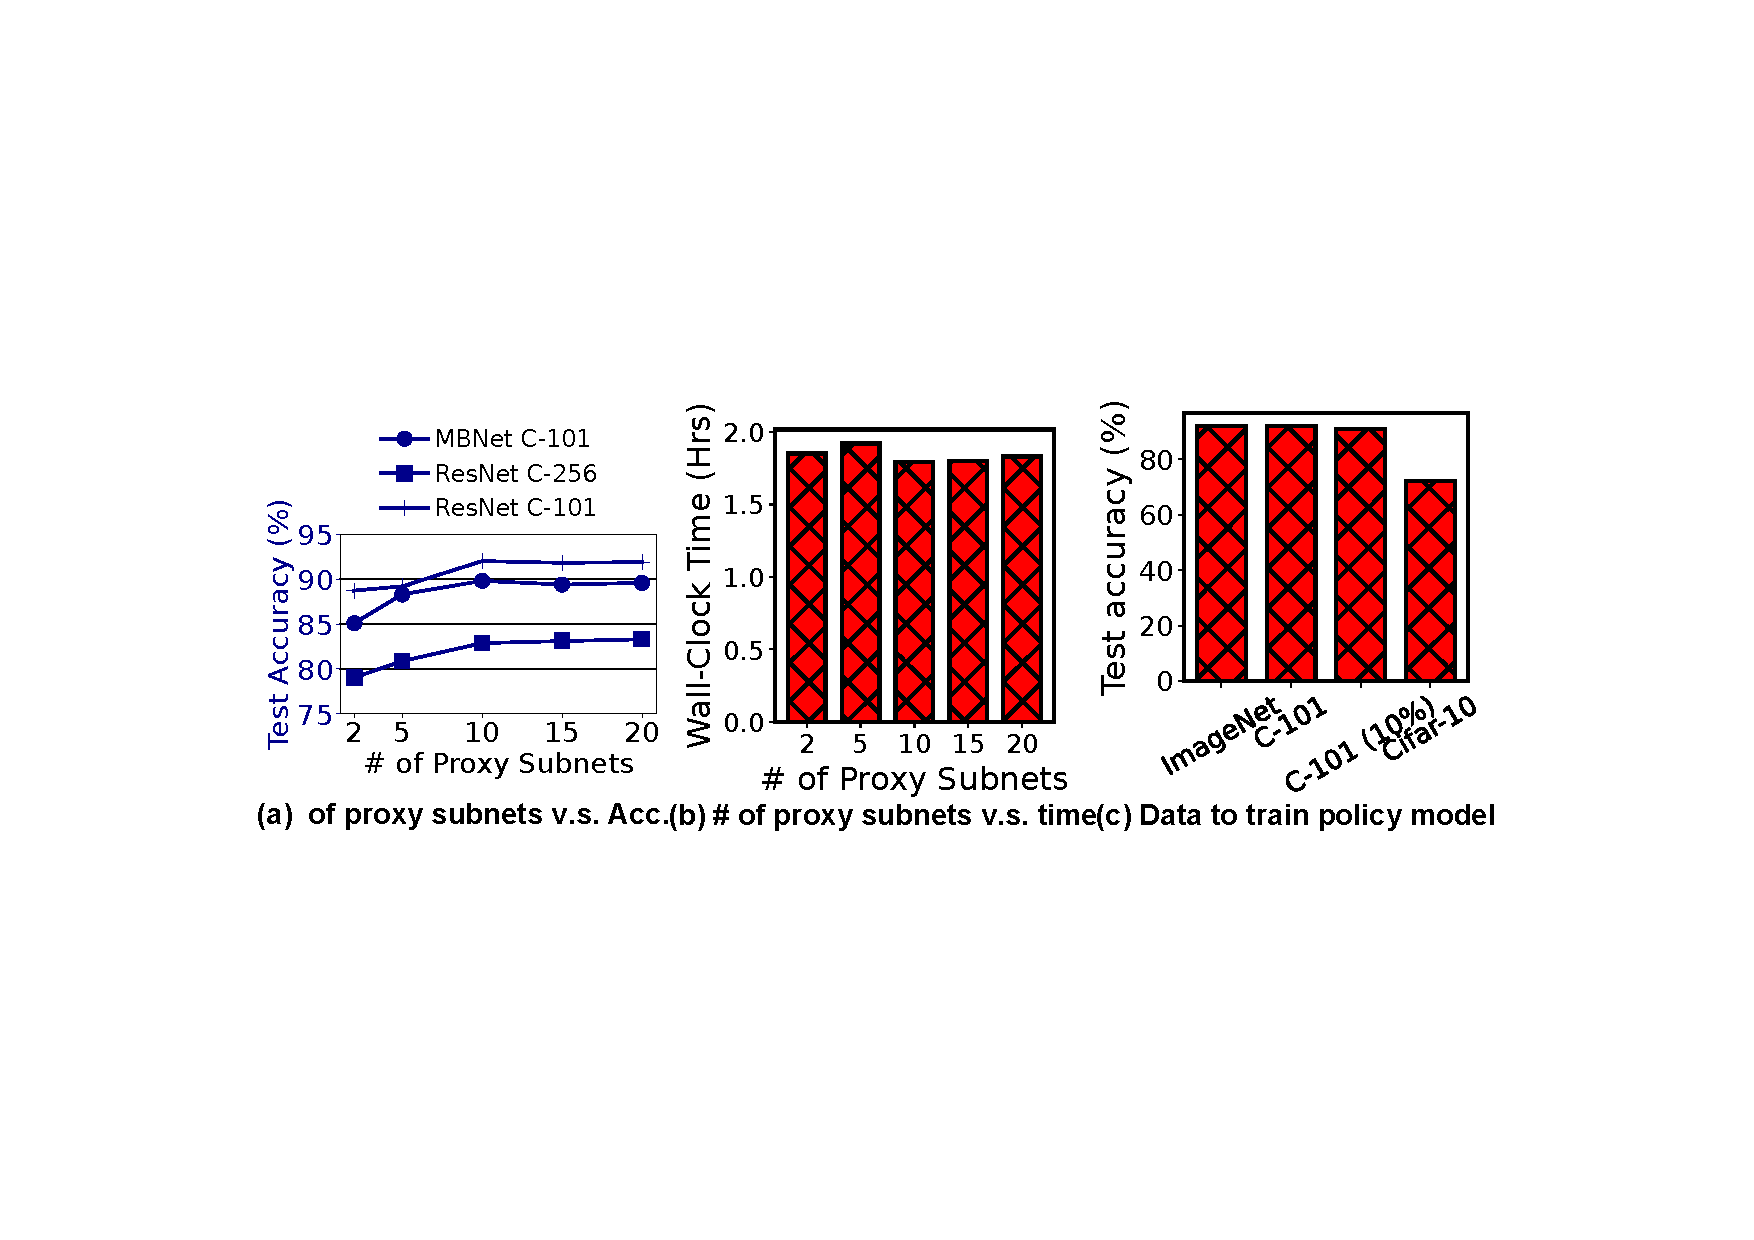
\includegraphics[width=0.98\linewidth]{figs/sensitivity.pdf}
    
    \caption{Sensitivity analysis.}
    
    \label{fig:sensitivity}
\end{figure}


\begin{figure}[!t]
    \centering
    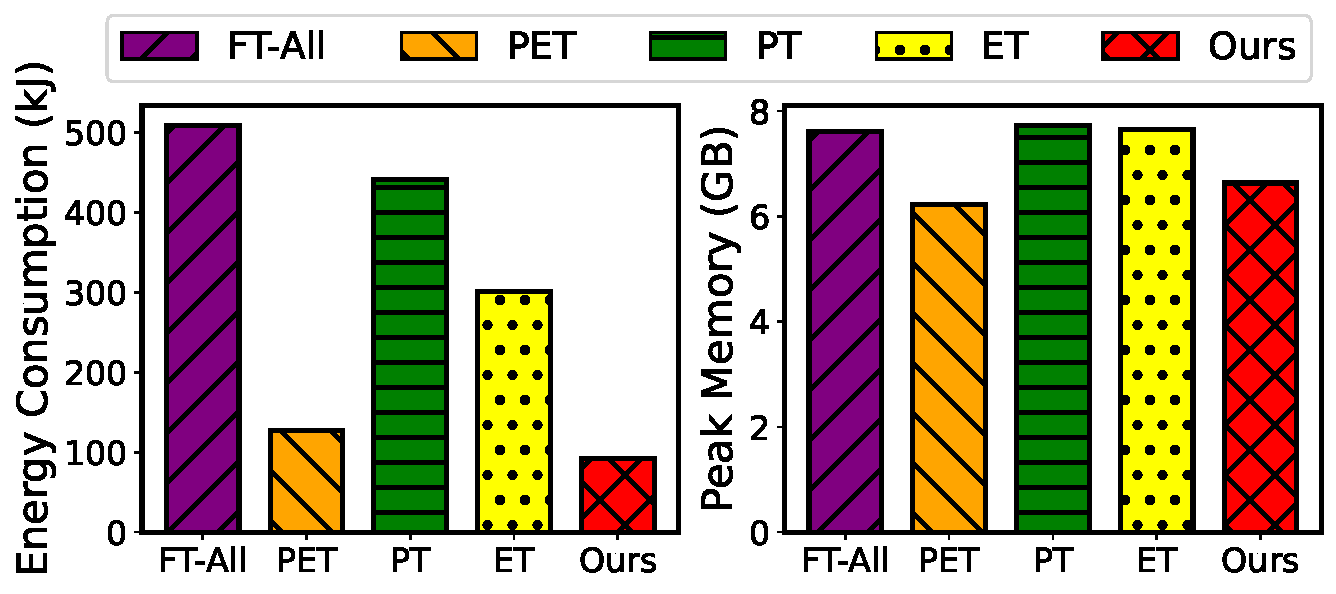
\includegraphics[width=0.82\linewidth]{figs/energyandmemory.pdf}
    
    \caption{Energy and memory consumption. }
    
    \label{fig:energy}
    \label{fig:memory and energy}
\end{figure}

\subsection{Energy and Memory Consumption}
\label{subsec: energy}
In this section, we report the energy and memory consumption of \sys against its baselines.
We train ResNet50 on Caltech-101 dataset with Jetson TX2.
We obtain energy/memory consumption by jtop~\cite{jtop}.
The results are shown in Figure~\ref{fig:energy}.

\noindent \textbf{Energy consumption.} 
\sys reduces energy consumption by 5.53$\times$/1.28$\times$ compared to \texttt{FT-All} and \texttt{PET}.
This is attributed to \sys's time efficiency, since \sys achieves better time-to-accuracy.
However, compared to \sys's training time reduction, the energy reduction is slightly lower.
This is mainly due to \sys periodically loads proxy sub-networks from disk ($\S$\ref{subsec:data-aware training}), which is also energy consuming.

\noindent \textbf{Memory consumption.}
We have the following observations.
(1) Both \texttt{PET} and \sys consumes fewer memory than \texttt{FT-All}/\texttt{PT}/\texttt{ET}.
The measured reduction is less than theoretical. 
This is mainly due to pytorch framework loads some runtime packages to memory, and does not prioritize memory saving operations such as in-place computation and buffer-reuse.
(2) \sys consumes more memory than vanilla \texttt{PET}.
This is because \sys uses additional memory for swapping.

\subsection{NPU Acceleration}
\label{subsec:NPU}

\begin{figure}[!t]
	\centering
	\begin{minipage}[b]{0.96\linewidth}
		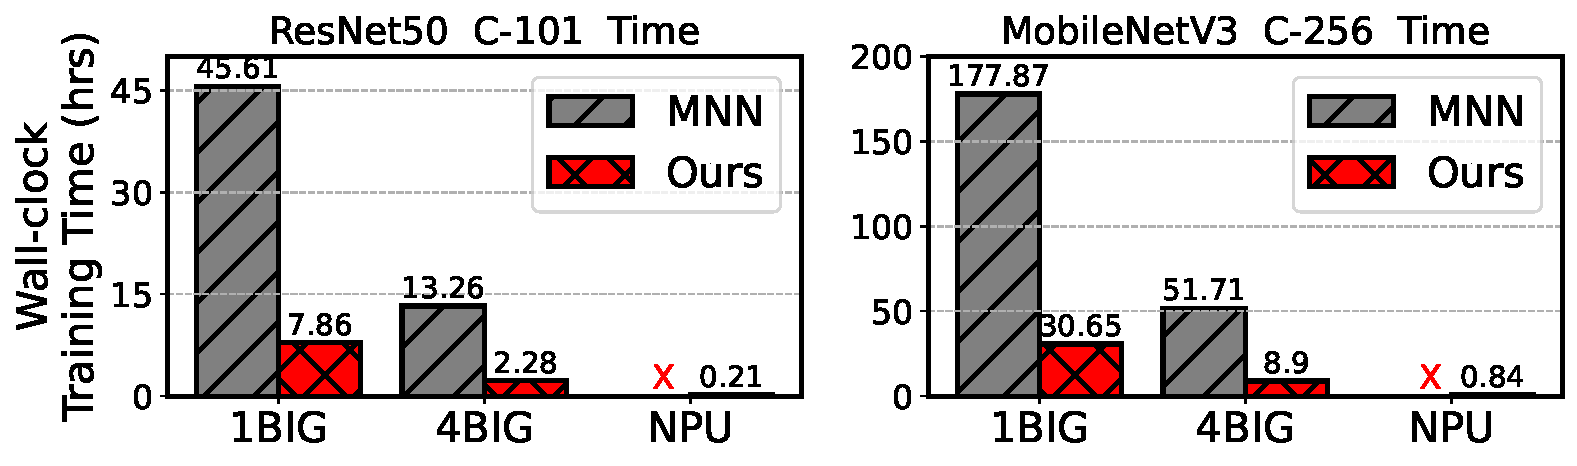
\includegraphics[width=\linewidth]{figs/NPU_time.pdf}
		
		\label{fig:resnet}
	\end{minipage}
	\begin{minipage}[b]{0.96\linewidth}		
            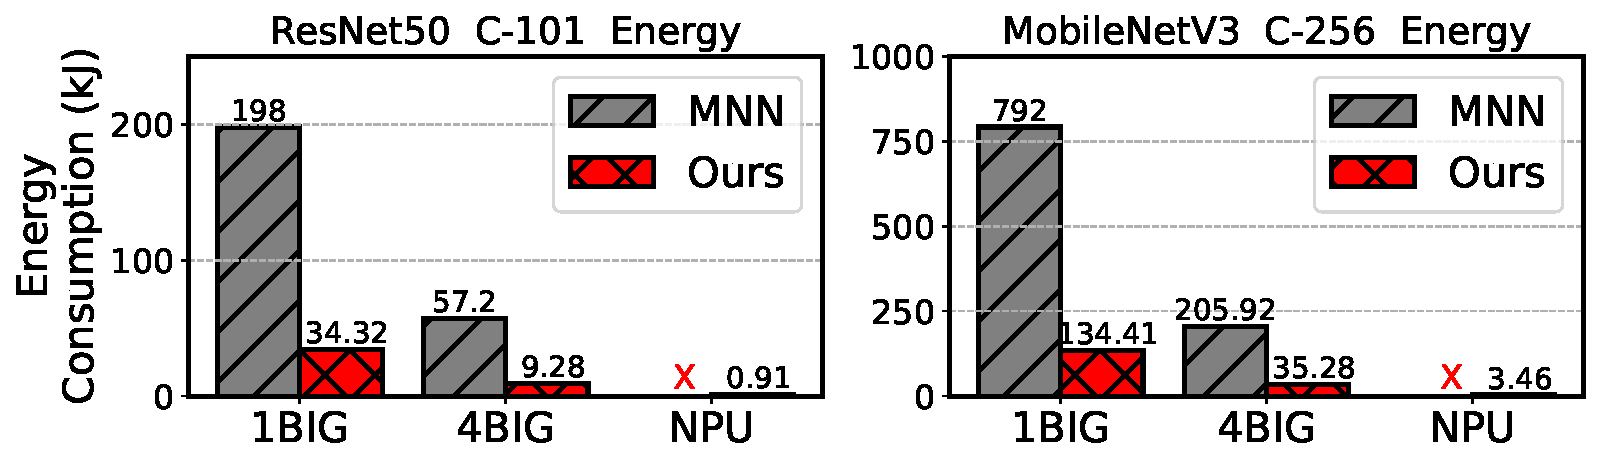
\includegraphics[width=\linewidth]{figs/NPU_energy.pdf}
		
		\label{mbnet}
	\end{minipage}
        
	\caption{Performance on COTS devices with different processors compared to MNN. ``1BIG'', ``4BIG'' and ``NPU'' are run on Huawei Mate30 with 1 CPU big core, 4 CPU big cores and NPU, respectively. ``X'' means not supported.}
         
        \label{fig:NPU}
\end{figure}

Commercial off-the-shelf mobile devices typically integrate various processors into their SoCs for different purposes, such as CPU, GPU, DSP, ISP, NPU, etc.\footnote{Mobile GPUs have been proven unsuitable for DNN training~\cite{das2022enabling}, and DSPs, due to their low-precision (INT8/INT4) computing characteristics, can only be used for training from scratch instead of fine-tuning pre-trained weights~\cite{xu2022mandheling}.} 
While NPUs offer high-precision (FP32/FP16) AI computing ability, their operators and software stacks are closed-source and only inference-friendly (e.g., only high-level non-configurable ABIs available for Kirin NPUs~\cite{Hiai}).
% So there is a gap between NPU and fine-tuning.

Fortunately, \sys's design is NPU-friendly, as its frozen subnets can reuse NPU operators and software stacks for acceleration, while trainable blocks that require weight updates can still be computed on the CPU.
This is a ``syntactic sugar'' at the implementation level, completely orthogonal to the core design of \sys.

We run \sys on a HuaiWei Mate30 smartphone with Kirin 990 half-precision (FP16) NPU, and compare its performance to a popular on-device training framework MNN~\cite{MNN}. 
The default fine-tuning strategy of MNN is full model fine-tuning with 4 CPU big cores.
As is shown in Figure ~\ref{fig:NPU}, with the assistance of key techniques in \sys and NPU offloading, on-device fine-tuning becomes practical and even efficient:
a medium-sized fine-tuning workload (ResNet50, Caltech-101) requires only 0.21 hours and 0.91 kJ of energy, whereas MNN takes 13.26 hours and 57.2 kJ of energy. 
On much larger datasets (Caltech-256), \sys also requires only 0.84 hours and 3.46 kJ of energy.

% Shared setup for the four-condition, full-12-epoch Orin experiment.
% Evidence: ../orin_scheduling/results/feature_20261113_prefetch_full_v2/
\begingroup
\color{blue}
\subsection{Coexisting with Periodic Inference on Jetson Orin}
\label{subsec:orin-periodic}

\begin{table*}[!t]
\color{blue}
\caption{Experiment on Jetson orin with a periodic forground inference workload.}
\label{tab:orin-prefetch}
\centering
\footnotesize
\setlength{\tabcolsep}{4pt}
\renewcommand{\arraystretch}{1.10}
\arrayrulecolor{blue}
\begin{tabular}{@{}lrrrrr@{}}
\toprule
Method & \makecell{Training\\(s)} & \makecell{Training time\\saved (\%)} & \makecell{Accuracy\\(\%)} & \makecell{Inference\\p99 (ms)} & \makecell{Misses\\(\%)} \\
\midrule
FIFO & 737.05 & 0.00 & 91.85 & 26.56 & 0.0042 \\
Reorder & 664.70 & 9.82 & 91.85 & 25.88 & 0.0000 \\
FIFO + prefetch & 569.53 & 22.73 & 91.92 & 26.69 & 0.0134 \\
Reorder + prefetch & 517.06 & 29.85 & 91.39 & 26.02 & 0.0046 \\
\bottomrule
\end{tabular}
\arrayrulecolor{black}
\end{table*}

We test whether reordering training work and computing features ahead of time can speed up background training while foreground inference runs regularly.
We compare four methods: FIFO, Reorder, FIFO with prefetching, and Reorder with prefetching.
FIFO without feature caching is the baseline.
Both optimizations run on the device and leave offline proxy generation and policy training unchanged.

\noindent \textbf{Setup.}
We use a Jetson AGX Orin developer kit with 64\,GB memory in its existing 30\,W power mode.
It runs PyTorch 2.0.0+nv23.05 and CUDA 11.4.
We use the released ResNet50 proxy networks, policy model, and classifier on Caltech-101.
The proxy networks stay frozen, and we train the classifier for 12 epochs with batch size four and an SGD learning rate of 0.001.
All methods use the same models and store tensors in FP32.
We turn off the Python TF32 settings, although the released TorchScript convolution operators still allow TF32 internally.

For the four-method comparison, a foreground inference request arrives every 105\,ms during training.
We measure its response time from its scheduled arrival until the GPU finishes it, including any waiting time.
We set a response-time target of 33.20\,ms before the experiments and process every request.

\noindent \textbf{Scheduling.}
We use the FIFO and Reorder rules in Section~\ref{subsec:reorder}.
All four methods give foreground requests priority and leave a 2\,ms safety margin before the next request.
Reorder looks ahead by up to 128 batches.
Without caching, it stops letting later batches pass the oldest batch after eight such passes.
With caching, only feature computation is reordered; the remaining training work keeps the original batch order.

We estimate how long each operation will take from measured runtimes.
The initial estimate is 1.15 times the 95th-percentile runtime measured without foreground inference.
We then update it to 1.10 times the 95th percentile of the latest 32 measurements, but never below the initial estimate.
For any operation that may update the classifier, we reserve enough time for a full backward update before deciding whether the loss calls for one.

\noindent \textbf{Timing.}
Each reported result comes from one run.
We use a fixed seed to shuffle the run order within each experiment.
Each run starts from the same classifier and routing state and uses the same random seed.
Training time covers all 12 training epochs, including waiting time and scheduling overhead, but excludes evaluation.
Total time also includes the 12 full evaluations and the time needed to finish any remaining foreground requests.
We load the models and prepared images into GPU memory before timing starts.
Initial policy inference, runtime measurements for the starting estimates, and warmup also take place before timing starts.
We check the logs to confirm that all training batches, evaluations, and foreground requests finish, that batches follow the required order, and that the recorded times are consistent.
\par
\endgroup


% Generated only from complete, verified full-12-epoch measurements.
% Evidence: ../orin_scheduling/results/feature_20261113_prefetch_full_v2/
\begingroup
\color{blue}
\noindent\textbf{Prefetching.}
We compute features for upcoming batches before the classifier needs them, as described in Section~\ref{subsec:feature-prefetch}.
We look ahead by up to 128 batches and reserve space for at most 32 batches of features.
A single forward call can process one, two, or four batches that use the same proxy.
The classifier still uses batches of four images and updates in the original order in both prefetch methods.
Each selected training image passes through its assigned proxy once per epoch.
We use each feature once and then release it; the next epoch computes new features.
Evaluation also recomputes its features.
All prefetch work counts toward training time, from preparing the first features to using the last ones.



\noindent\textbf{Results.}
Table~\ref{tab:orin-prefetch} shows the results. Accuracy is measured after epoch 12. A miss means that an inference request takes more than 33.20\,ms to finish.
Compared with FIFO without caching, Reorder alone cuts training time by 9.82\%.
Adding prefetching to FIFO cuts it by 22.73\%, and combining Reorder with prefetching cuts it by 29.85\%.
On top of FIFO with prefetching, reordering feature computation reduces training time by a further 9.21\%.

Final accuracy is 91.85\% for FIFO without caching, 91.92\% for FIFO with prefetching, and 91.39\% for Reorder with prefetching.
The combined method is 0.46 percentage points below the baseline. These runs do not establish that the methods reach the same final accuracy.
The feature buffer uses at most 359.38\,KiB in these runs. This excludes memory for models, inputs, and operator workspaces.


\par
\endgroup


% Generated from verified 12-epoch measurements; do not insert smoke timings.
% Provenance: ../orin_scheduling/period_sweep_protocol.txt
\begingroup
\color{blue}
\noindent\textbf{Varying the foreground inference period.}
We compare FIFO without caching and Reorder with prefetching at request periods of 105, 135, and 180\,ms.
Figure~\ref{fig:orin-period-sweep} reports the time for all 12 training epochs, excluding evaluation, using the same settings as above.
The 105\,ms results are reused from Table~\ref{tab:orin-prefetch}; we run both methods once at each of the other two periods.
Reorder with prefetching reduces training time at all three periods, by 23.97--29.85\% in these runs.
The benefit therefore persists across the tested request periods.


\begin{figure}[!t]
\color{blue}
\centering
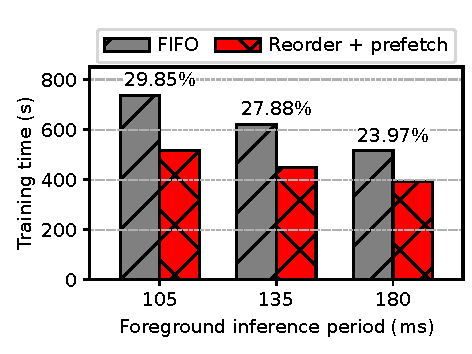
\includegraphics[width=80mm]{figures/orin_period_sweep.pdf}
\caption{Training time under different foreground inference periods. Bars show the time for 12 training epochs, excluding evaluation. Percentages show the reduction relative to FIFO without caching.}
\label{fig:orin-period-sweep}
\end{figure}
\par
\endgroup


\section{Related Work}
\noindent \textbf{Time-efficient on-device training.}
A considerable amount of literature/frameworks have investigated how to enable and accelerate training on resource-constrained edge devices~\cite{huang2023elastictrainer, xu2022mandheling, 10.1145/3295500.3356156, mercury2021sensys, 10.1145/3384419.3430716, zhu2023pockengine, tflite, tfjs, MNN}.
For instance, ElasticTrainer~\cite{huang2023elastictrainer} reduces training time by non-deterministically training a portion of the network.
Mandheling~\cite{xu2022mandheling} directly downsamples the entire network and maps it to the hardware accelerator.
There are also many open-source frameworks tailored for on-device training, such as TFLite~\cite{tflite} from Google and MNN~\cite{MNN} from Alibaba.
\sys is compatible with the above frameworks and hardware accelerator oriented works.
The difference between \sys and other works, such as ElasticTrainer and PruneTrain, which also employ dynamic neural network architectures, lies in \sys not compromising on parameter efficiency.

\noindent \textbf{Neural network compression/approximation.}
Neural network compression/approximation refers to approximating the original network with simpler and lighter networks, which can come from network structure approximation (e.g., structural pruning~\cite{torchpruninggithub, krishnan2019structural, AdaSpring, AdaEnlight} or sparse weights~\cite{tangandyang2023torchsparse}) or data precision approximation (e.g., INT8/INT4 quantization~\cite{frantar2023gptq, Zafrir_2019}).
% Although these works can reduce the over-parameterization on a certain downstream task and statically generate a more compact network, they compromise the generality on other tasks.
Different from the aforementioned works, \sys's NN approximation is dynamic for each data point, and is accurate enough for lossless training.

\noindent \textbf{Foundation models as a mobile system service.}
Compared to traditional on-device AI paradigm that individually deploys a compact model for each task~\cite{yin2024llmservicemobiledevices, cai2018proxylessnas, cai2018proxylessnas, Fang_2018, lu2024smalllanguagemodelssurvey, xu2024surveyresourceefficientllmmultimodal, yin2024elmselasticizedlargelanguage}, recent advances in LLMs~\cite{zhou2023large, muennighoff2023crosslingual, BELLE, koala_blogpost_2023, brown2020language} and multimodal~\cite{tang2023anytoany, su2023pandagpt, radford2021learning, li2021align, li2022blip, li2023blip2} suggest that a highly parameterized 
OS-level foundational model~\cite{yuan2023rethinking, yang2023edgefm} with stronger generalization and emergent capabilities is more suitable for the evolving workloads in on-device AI.
\sys sheds light on building such a one-for-all foundation ML system on devices to continuously and personally serve ubiquitous AI tasks.

\noindent \textbf{Routing diverse data to multiple networks.}
\yws{
Several prior arts~\cite{tabi, li2021appealnetefficienthighlyaccurateedgecloud, kag2023efficient} also leverage the idea of routing diverse data to multiple networks that has diverse compute cost.
Appealnet~\cite{li2021appealnetefficienthighlyaccurateedgecloud} proposes a two-head little network for routing data to two cascaded big-little networks at inference time.
The difficulty in Appealnet is defined as a loose measurement on softmax probability.
Selective Query~\cite{kag2023efficient} trains a routing model for assigning the to-be-inferenced sample to either the cloud or the device.
These work mainly focus on \textit{inference} optimizations, which are much more simple and deterministic compared to training.
\sys's data routing identifies several unique aspects in training, including feature-level difficulty and training sample importance to convergence.
}

\section{Discussion}
\label{subsec: discussion}

\textbf{Data diversity.}
\yws{
\sys is the first work to identify and orchestrate data difficulty and importance to dynamically approximate the frozen layers of PET.
Although there are some early efforts~\cite{teerapittayanon2017branchynetfastinferenceearly, baldock2021deeplearninglensexample} that explore the diversity, their definition cannot be directly applied to PET mainly due to the following reasons.
Firstly, they mainly focus on reducing the inference-time overhead by layer-level early exit for diverse samples.
NN inference has a higher tolerance for extracted features.
For instance, when a feature is tortured, one classification network can still output the correct answer if the highest logit is in the label class, regardless the other classes.
While in training, this may lead to a severely affected convergence.
Instead, \sys sets stringent restriction for training by a feature-level matching in its difficulty definition.
Secondly, early exiting is essentially a pruning method with sequential layer-level heuristic, which is much more coarse-grained than \sys's IDC pruning that prunes neurons in independent dimensions.
}
% \mwx{(1) SOTA data diversity definition methods. (2) their drawbacks (3) Ours's difference.}

\noindent \textbf{Handling diversity distribution drift.}
\yws{
One practical issue that \sys faces in real-world deployment is the data diversity distribution drift.
As \sys focuses on on-device fine-tuning, the distribution of on-device data may differ from on-cloud pre-training data.
To this end, \sys has the following conclusions and alternatives.
Firstly, as elaborated in $\S$\ref{subsec: sensitivity} and $\S$\ref{subsubsec:policy model}, the pattern of data difficulty is much more simple and deterministic than the distribution on concrete tasks, thus showing strong transferablity.
For instance, an NN trained on ImageNet still needs fine-tuning on caltech-101 dataset, while the difficulty pattern that captured by \sys's policy model on ImageNet has been nearly equivalent to caltech-101.
Besides, \sys has several alternatives when the fine-tuning data is completely different from pre-training.
One can crowd-sourcing a portion of user-permitted trainable data to the cloud, federated learning the policy model, or directly on-device continuously training the policy model.
}

\noindent \textbf{Other approximation techniques.}
\yws{
Here we discuss the design philosophy behind \sys on choosing the approximation technique.
Sparsity and quantization is not a good fit for \sys, as they can only provide a limited wall-clock speedup on mobile SoC processors.
For instance, to the best of our knowledge, the Raspberry Pi has no dedicated compute units for quantized data formats like int4.
Thereby, a highly quantized network only achieves an insignificant speedup on these devices since most of its operators are compute-bound.
Sparsity is also not well-supported on mainstream mobile SoCs.
Early exiting is essentially a coarse-grained pruning, thus also sub-optimal compared to pruning.
\sys employs structural pruning, which is the most suitable technique direction for PET acceleration on mobile devices.
}

\noindent \textbf{Applicability to language models.}
\yws{
Currently, \sys is mainly designed for on-device tuning CV models.
The LLMs are typically much heavier than CV models (e.g., llama-7B), and their fine-tuning on extremely resource-constrained mobile devices is still not a practical solution for demands like personalization.
Nevertheless, the main techniques of \sys are generally applicable to LLMs, with minor adjustments like supporting LoRA structures and profiling token-level data diversity.
We leave this as our future work.
}
\section{Conclusion}

This work has proposed \sys, a framework for time-efficient on-device parameter efficient training.
It innovatively leverages data diversity and neural network approximations for reducing the computation cost of frozen layers.
\sys achieves up to 2.5$\times$ on-device fine-tuning speedup compared to state-of-the-art PET methods, and up to 6.6$\times$ speedup compared to traditional full model fine-tuning.
\sys makes on-device fine-tuning more practical for COTS devices equipped with NPUs.

\section*{Acknowledgments}
This work was supported by National Natural Science Foundation of China under the grant number 62325201, and Center for Data Space Technology and System, Peking University.


\bibliographystyle{IEEEtran}
\bibliography{ref}
\end{document}
